% SETTINGS

\newcommand{\myTitle}[0] {Uplatnenie interpretovateľnosti a vysvetliteľnosti neurónových sietí pri vyhodnocovaní medicínskych obrazových dát}
\newcommand{\myTitleEng}[0] {Application of interpretability and explainability of neural networks in the evaluation of medical images}
\newcommand{\myName}[0] {Bc. Timotej Zaťko}
\newcommand{\mySupervisor}[0] {Ing. Martin Tamajka}
\newcommand{\mySupervisorEng}[0] {Ing. Martin Tamajka}
\newcommand{\myEvidenceNumber}[0] {FIIT-182905-86077}
\newcommand{\myDate}[0] {Máj 2021}
\newcommand{\myStudyProgram}[0] {Inteligentné softvérové systémy}
\newcommand{\myStudyProgramEng}[0] {Intelligent Software Systems}
\newcommand{\myDegreeCourse}[0] {Informatika}
\newcommand{\myDegreeCourseEng}[0] {Computer Science}
\newcommand{\myInstitute}[0] {Ústav počítačového inžinierstva a aplikovanej informatiky (FIIT)}
\newcommand{\myFontSize}[0] {12pt}
\newcommand{\mySpacing}[0] {1.3}
\newcommand{\myBibliography}[0] {bibliography/references}

% \documentclass[\MyFontSize,a4paper,twoside,openright,english]{book}
\documentclass[12pt,a4paper,twoside,openright,english]{book}
\usepackage[utf8]{inputenc}
\usepackage[T1]{fontenc}
\usepackage[english,slovak]{babel}
\usepackage[a4paper]{geometry}

\usepackage[parfill]{parskip}
\usepackage{enumitem}

\usepackage{graphicx}
\usepackage{float}
\usepackage{longtable}
\usepackage{setspace}
\usepackage{listings}
\usepackage{xparse}
\usepackage{caption}
\usepackage{hyperref}
% \usepackage[hyphenbreaks]{breakurl}
\usepackage{pifont}
\usepackage[titletoc]{appendix}
\usepackage{tocloft}
\usepackage{csquotes}


% Spacing
% \setstretch{\mySpacing}
\setstretch{1.3}

\setcounter{secnumdepth}{3}
\setcounter{tocdepth}{3}

\usepackage{tabularx}
\newsavebox\mybox
\usepackage{fancyhdr}
\pagestyle{fancy}
\lhead{\nouppercase{\leftmark}}
\chead{}
\rhead{}
\lfoot{}
\cfoot{\thepage}
\rfoot{}

%style=iso-numeric
%style=authortitle-dw
% \usepackage[backend=bibtex,defernums=true]{biblatex}

\usepackage[
   backend=biber        % if we want unicode
  ,style=iso-numeric % or iso-numeric for numeric citation method
  ,autolang=other       % to support multiple languages in bibliography
  ,sortlocale=sk     % locale of main language, for sorting
  ,bibencoding=UTF8     % this is necessary only if bibliography file is in different encoding than main document
]{biblatex}

\defbibheading{references}[References]{ 
  \chapter*{#1}
  \markboth{#1}{#1}
}
\defbibheading{referencessec}[References]{ 
  \section*{#1}
  \markboth{#1}{#1}
}
% \bibliography{\myBibliography}
\bibliography{bibliography/references}
% \addbibresource{bibliography/references.bib}

% Listing as figure
% \usepackage{libs/minted}
% \usepackage[section]{minted}

\usepackage{listing}

% openright does not work :(
\let\tmp\oddsidemargin
\let\oddsidemargin\evensidemargin
\let\evensidemargin\tmp
\reversemarginpar

\usepackage{lscape}
\usepackage{afterpage}

\usepackage{lipsum}

% Get rid of "Chapter N."
\makeatletter
\def\@makechapterhead#1{%
  \vspace*{50\p@}%
  {\parindent \z@ \raggedright \normalfont
    \interlinepenalty\@M
    \Huge\bfseries  \thechapter.\quad #1\par\nobreak
    \vskip 40\p@
  }}
\makeatother
%%%%%

% Table
\usepackage[table,xcdraw]{xcolor}
\usepackage{tabularx}

% Incldue pdf in document
\usepackage[final]{pdfpages}  

\addto\captionsenglish{\renewcommand{\figurename}{Obr.}}
\addto\captionsenglish{\renewcommand{\tablename}{Tabuľka}}

\lstdefinestyle{BashInputStyle}{
  language=bash,
  basicstyle=\small\sffamily,
  numbers=left,
  numberstyle=\tiny,
  numbersep=3pt,
  frame=tb,
  columns=fullflexible,
  backgroundcolor=\color{lightgray!20},
  linewidth=0.9\linewidth,
  xleftmargin=0.1\linewidth
}

\raggedbottom

% \renewcommand{\appendixname}{Príloha}


\begin{document}
    \captionsetup{justification=centering, margin=1cm}
    
    % Minted
    % pygmentize -L styles
    % \usemintedstyle{autumn}
    
    % Cover page
    \pagenumbering{roman}

% Tato strana pri tlaceny v tvrdej vazbe
\begin{center}
\thispagestyle{empty}
{\Large Slovenská technická univerzita v Bratislave}
\par\end{center}{\Large \par}

\begin{center}
{\Large Fakulta informatiky a informačných technológií}
\par\end{center}{\Large \par}

\smallskip{}

\begin{center}

% Toto pri final odovzdani odkomentovat 
\myEvidenceNumber

\par\end{center}
\vfill{}

\begin{center}
\textbf{\Large \myName}
\par\end{center}{\Large \par}

\medskip{}


\begin{center}
\textbf{\LARGE \myTitle }
\par\end{center}{\huge \par}

\medskip{}


\begin{center}

% Toto pri final odovzdani vymenit
% {\Large Priebežná správa o riešení DP2}
 {\Large Diplomová práca}

\par\end{center}{\Large \par}

\vfill{}

% Vedúci práce: \mySupervisor

\medskip{}
\myDate


\newpage
\thispagestyle{empty}
\mbox{}
\newpage
    
    % Title page
    \pagenumbering{roman}

\begin{center}
\thispagestyle{empty}
{\Large Slovenská technická univerzita v Bratislave}
\par\end{center}{\Large \par}

\begin{center}
{\Large Fakulta informatiky a informačných technológií}
\par\end{center}{\Large \par}

\smallskip{}

\begin{center}

% Toto pri final odovzdani odkomentovat 
\myEvidenceNumber

\par\end{center}
\vfill{}

\begin{center}
\textbf{\Large \myName}
\par\end{center}{\Large \par}

\medskip{}


\begin{center}
\textbf{\LARGE \myTitle }
\par\end{center}{\huge \par}

\medskip{}


\begin{center}

% Toto pri final odovzdani vymenit
% {\Large Priebežná správa o riešení DP2}
 {\Large Diplomová práca}

\par\end{center}{\Large \par}

\vfill{}

Študijný program: \myStudyProgram

Študijný odbor: \myDegreeCourse

Miesto vypracovania: \myInstitute

Vedúci práce: \mySupervisor

\medskip{}

\myDate


\newpage
\thispagestyle{empty}
\mbox{}
\newpage


    
    % Zadanie diplomovej prace
    % \includepdf[pages=1]{assets/thesis_assignment.pdf}

\thispagestyle{empty}
\mbox{}
\newpage
    
    % Cestne prehlasenie
    \thispagestyle{empty}
\mbox{}\vfill
\noindent Čestne vyhlasujem, že som túto prácu vypracoval samostatne, na základe konzultácií a s použitím uvedenej literatúry.
\\
\\
\\

\noindent V Bratislave, 17. máj 2021\\

\hfill Timotej Zaťko \hspace{6mm}

\newpage\null\thispagestyle{empty}\newpage


    
    % Annotation
    %
% ANNOTATION - SK
%

% https://www.fiit.stuba.sk/buxus/docs/organizacia_studia/pokyny/ZP-clenenie-pokyny.pdf

\thispagestyle{empty}
\section*{Anotácia}

\begin{minipage}[t]{1\columnwidth}%
Slovenská technická univerzita v Bratislave

Fakulta informatiky a informačných technológií

Študijný program: \myStudyProgram\\

Autor: \myName

Diplomová práca: \myTitle

Vedúci diplomového projektu: \mySupervisor

máj 2021
\end{minipage}

\bigskip{}

Súčasný vplyv umelej inteligencie na spoločnosť je nespochybniteľný. Využitie si už našla v rôznych oblastiach našich životov či už je to v smartfónoch pri odomykaní tvárou alebo najnovšie pri kontrole používania ochranného rúška pri vstupe do obchodov. Umelá inteligencia sa postupne dostáva do oblasti medicíny, kde má potenciál zachraňovať životy. Aby sa stala spoľahlivým pomocníkom doktorov pri diagnóze ochorení, je nevyhnutné, aby jej rozhodnutia bolo možné vysvetliť. 

V oblasti medicíny je možné použitie neurónových sietí, pretože dokážu veľmi dobre pracovať s obrazovými dátami, a tak sa dajú využiť napríklad pri diagnóze Alzheimerovej choroby z rádiologických snímiek. Ich problémom však je, že sa správajú ako "čierne skrinky" čo bráni ich použitiu v bežnej praxi.

V tejto práci sme navrhli a implementovali novú metódu vysvetľovania rozhodnutí neurónových sietí, ktorá vychádza z už existujúcej metódy - RISE. Vytvorená metóda je vhodná pre obrazové dáta, ku ktorým vytvára tepelné mapy vysvetľujúce rozhodnutia modelu.

Metódu sme overili na neurónovej sieti deketujúcej Alzheimerovu chorobu z MRI snímiek a porovnali ju voči pôvodnej metóde a iným existujúcim metódam. Nová metóda síce dosiahla oproti pôvodnej lepšie výsledky, avšak sa neukázala byť vhodná pre rádiologické dáta.

\newpage
\thispagestyle{empty}
\mbox{}
\newpage

%
% ANNOTATION - ENG
%

% https://www.fiit.stuba.sk/buxus/docs/organizacia_studia/pokyny/ZP-clenenie-pokyny.pdf

\thispagestyle{empty}

\section*{Annotation}

\begin{minipage}[t]{1\columnwidth}%
Slovak University of Technology Bratislava 

Faculty of Informatics and Information Technologies

Degree Course: \myStudyProgramEng\\

Author: \myName

Diploma's Thesis: \myTitleEng

Supervisor: \mySupervisorEng

2021, May
\end{minipage}

\bigskip{}

The current impact of artificial intelligence on society is undeniable. It has already been used in various areas of our lives, whether it is in smartphones for unlocking via face recognition or, most recently, for controlling the use of protective masks when entering shops or groceries. Artificial intelligence is entering the field of medicine, where it has the potential to save lives. Thus, in order to be a reliable assistant to doctors for example in the diagnosis of the disease, it is necessary that its decisions can be explained.

Since neural networks perform well on image data, they can be used in the field of medicine, for example, in the diagnosis of Alzheimer's disease from radiological images. However, their problem is that they behave like a "black box" which prevents their adoption into common practice.

In this work, we designed and implemented a novel method for explaining neural network decisions, which is based on other existing method - RISE. The created method is suitable for image data, for which it creates heatmaps explaining the decisions of the model.

We have validated the method on a neural network detecting Alzheimer's disease from MRI images and compared it to the original, and other existing methods. Although the new method achieved better results than the original, it did not prove to be suitable for radiological data.

\newpage
\thispagestyle{empty}
\mbox{}
\newpage

    
    % Acknowledgment
    % Poďakovanie

\thispagestyle{empty}
\mbox{}\vfill
\textbf{\Large Poďakovanie}

\noindent Ďakujem môjmu školiteľovi Ing. Martinovi Tamajkovi za odbornú pomoc a vedenie pri tvorbe tejto práce.
\\
\\
\\

\newpage\null\thispagestyle{empty}\newpage


    
    % Table of contents
    \pagenumbering{arabic}
    
    \renewcommand*\contentsname{Obsah}
    \tableofcontents

    % Dictionary of terms
    \chapter*{Zoznam použitých skratiek}

\paragraph{AD} angl. Alzhemier disease (Alzheimerova choroba) -- používa sa na označenie pacientov trpiacich Alzheimerovou chorobou
\paragraph{AUC} angl. area under curve (plocha pod krivkou)
\paragraph{CN} angl. cognitive normal (kognitívne zdravý) -- používa sa na označenie pacientov bez kognitívneho poškodenia (tj. zdravých jedincov)
\paragraph{MCI} angl. mild cognitive impairment (mierne kognitívne poškodenie) -- používa sa na označenie pacientov s miernym kognitívnym poškodením
\paragraph{MRI} angl. magnetic resonance imaging  (magnetická rezonancia ) -- je spôsob tvorby rádiologických snímkov ľudského tela, používa sa pri diagnostike Alzheimerovej choroby
\paragraph{PET} angl. positron emission tomography  (pozitrónová emisná tomografia) -- je spôsob tvorby rádiologických snímkov ľudského tela, používa sa pri diagnostike Alzheimerovej choroby
    
    % List of listings
    % \listoffigures\newpage{}
    % \renewcommand\listoflistingscaption{List of Listings}
    % \listoflistings\newpage{}
    
    % References segment
    \begin{refsegment}
    
    % Introduction
    % \clearpage\null
    % \input{content/intro}
    
    % Introduction
    % \clearpage\null % This makes those blank pages between the chapters, the chapter begining is on the right side and on the left is a blank page
    \setcounter{page}{1}
    \chapter{Úvod}

% Uvod
% Spomenut neuronove siete, preco sa pouzivaju, preco ich ideme pouzit.
% Co robime, preco a ako.

Umelá inteligencia sa už dávno stala súčasťou nášho každodenného života. Pri-chádzame s ňou do kontaktu neustále, keď odomykáme telefón vlastnou tvárou alebo keď pomocou prekladača prekladáme text to iného jazyka. 
% spomenut nieco ako smartfon, vyhladavanie, fotak (ai camera), prekladanie?
Jej využitie je tiež rozšírené v oblasti medicíny, kde má potenciál zachraňovať životy. Využíva sa pri výrobe liekov, monitorovaní zdravia, analýze zdravotných plánov, chirurgických zákrokoch a aj pri odhaľovaní chorôb \cite{amisha2019overview}.
Práve pri odhaľovaní chorôb sa častokrát využívajú hlboké neurónové siete, a to napríklad pri detekcii rakoviny kože, rakoviny pľúc alebo Alzheimerovej choroby z obrazových dát.
% Dat zdroje k jednotlivym chorobam?
% Lung Cancer - https://www.sciencedirect.com/science/article/pii/S0169260713003532
% Skin Cancer - https://www.nature.com/articles/nature21056
% Alzheimer Disease - https://link.springer.com/article/10.1007/s10916-018-0932-7

Neurónovým sieťam sa už podarilo dosiahnuť také dobré výsledky, že sú porovnateľné s expertmi v medicínskej oblasti.
% "performance on par with all tested experts across both tasks, demonstrating an artificial intelligence capable of classifying skin cancer with a level of competence comparable to dermatologists"
% https://www.ncbi.nlm.nih.gov/pubmed/28117445
Ich problémom však je, že sa správajú ako "čierna skrinka", čo v oblasti medicíny nie je žiadúce. Preto je nevyhnutné, aby boli rozhodnutia neurónovej siete interpretovateľné a pacient s lekárom vedeli, na základe čoho sa neúronová sieť rozhodla. Lekári by si mali svoje rozhodnutia vedieť obhájiť. Aby sa teda neurónové siete mohli stať bežným pomocníkom lekárov, je vysvetliteľnosť ich rozhodnutí dôležitá.
    
    % Analysis
    % \clearpage\null
    \chapter{Analýza}

\section{Alzheimerova choroba \label{sec:ad}}

Alzheimerova choroba je najčastejšou príčinou demencie. Prvotné príznaky tejto choroby sú zhoršenie pamäti, zabúdanie nedávnych udalostí, mien, neschopnosť rozoznávať známe miesta či orientovať sa v čase \cite{Alzheimer.sk_2019}. Jej priebeh sa vyznačuje postupným poklesom kognitívnych funkcií, postupným zhoršením pamäte, myslenia, rozprávania a schopnosti učenia sa \cite{duthey2013background}. Najčastejšie sa vyskytuje u ľudí starších ako 65 rokov, s pravdepodobnosťou výskytu až 50\% po dovŕšení 85 rokov života \cite{duthey2013background}.
% khan2016biomarkers uvadza 24–33%, dafuuuuq???
% Age is the strongest risk factor for LOAD. Epidemiological studies have found that <1% of individuals aged 60–65 years have AD, and the prevalence increas- es exponentially to 24–33% of individuals aged 85 years (Alzheimer’s Disease (AD)–World Health Organization). Another estimate found that among pa- tients affected with AD, 4% are under age 65, 6% are 65–74, 44% are 75–84, and 46% are 85 or older (Alzheimer’s disease facts and figures 2012). The inci- dence of AD increases exponentially with age, and females are disproportionally (2:1) more susceptible to AD compared to male.
S narastajúcim vekom človeka sa zvyšuje pravdepodobnosť ochorenia. Pravdepodobnosť ochorenia zvyšujú taktiež úrazy hlavy, poruchy prekrvenia mozgu, pozitívna rodinná anamnéza či vzdelanie (pretože ľudia s nižším vzdelaním majú väčšie riziko rozvoja tohto ochorenia) \cite{Alzheimer.sk_2019}. Toto ochorenie sa vyskytuje častejšie u žien ako u mužov, v pomere 2:1 \cite{khan2016biomarkers}.

Alzheimerova choroba nie je ``iba`` o strate pamäti, ale aj šiestou najčastejšou príčinou smrti v USA \cite{Figures_2017}. Medzi rokmi 2000 až 2017 sa počet úmrtí v USA viac ako zdvojnásobil \cite{Figures_2017}. Ľudia starší ako 65 rokov ktorým bola diagnostikovaná táto choroba sa v priemere dožívajú 4 až 8 rokov po jej diagnóze \cite{Figures_2017}.

% Spomenut Amyloid beta?

\subsection{Diagnostika Alzheimerovej choroby}

Alzheimerova býva diagnostikovaná kombináciou viacerých ukazovateľov. Pri ur-čovaní diagnózy sa používajú neuropsychometrické (kognitívne) testy, rádiologické snímky (angl. neuroimaging data), biologické ukazovatele a špecifické kritériá, na základe ktorých je možné vylúčenie iných chorôb u pacienta z jeho histórie vývoja ochorenia \cite{khan2016biomarkers}. T. Khan zadefinoval tieto ukazovatele do tzv. komplexného rámca pre diagnózu Alzheimerovej choroby (Obr. \ref{fig:alzheimer_diagnosis_scheme}). V súčastnosti sa v tejto oblasti skúmajú biologické ukazovateľe (ich identifikácia a použitie), keďže používanie (a teda aj vytvorenie) rádiologických ukazovateľov je drahé \cite{khan2016biomarkers} (vyžaduje si to zaškolený personál a vybavenie). Biologické ukazovateľe zatiaľ nie sú dostatočne spoľahlivé \cite{khan2016biomarkers}.
% COMPREHENSIVE ALZHEIMER’S DISEASE DIAGNOSTIC FRAMEWORK, chapter 2.7
% TODO: zadefinoval? dobre slovo?

\begin{figure}[h!]
\centering
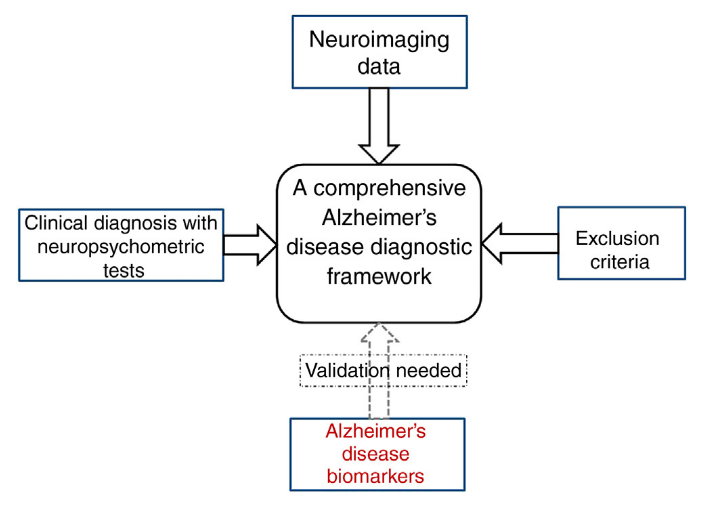
\includegraphics[scale=0.35]{assets/images/alzhemier_diagnosis_scheme.png}
\caption{\textbf{Komplexný rámec pre diagnózu alzheimerovej choroby}. Pozostáva z neuropsychometrických testov, rádiologických snímok (z PET, MRI...), biologických ukazovateľov (napr. úrovne hladín určitých proteínov v krvnej plazme) Alzheimerovej choroby a kritérií vylúćenia iných neurologických chorôb.\cite{khan2016biomarkers}}
\label{fig:alzheimer_diagnosis_scheme}
\end{figure}

\subsection{Biologické ukazovatele}
% angl. biomarkers

Biologické ukazovatele (angl. biomarkers) sú merateľné biologické ukazovatele slú-žiace na detekciu prítomnosti choroby.
% Toto by som najradsej odcitoval, pretoze tato veta je vyplodom precitani asi 5 zdrojov, ale vsade je to opisane velmi z "medical point of view" https://en.wikipedia.org/wiki/Alzheimer%27s_disease_biomarkers
National Insitute of Health definguje biologický ukazovateľ ako indikátor určitého objektívneho merania a hodnotenia biologického procesu, patogénneho procesu alebo farmakologického hodnotenia terapeutickej účinnosti \cite{working2001biomarkers}. Alzheimerova choroba môže byť identifikovaná sledovaním týchto biologických ukazovateľov napríklad v krvnej plazme \cite{khan2016biomarkers} alebo v mozgovomiechovej tekutine (angl. cerebrospinal fluid) (ako úrovne hladín proteínov P-tau and A$\beta$42) \cite{khan2016biomarkers} (angl. cerebrospinal fluid).

\subsection{Obrazové a rádiologické ukazovatele \label{sec:neoroimaging_biomarkers}}
% angl. image and radiogological markers, alebo neuroimaging
% ako prelozim neuroimaging???

Identifikovanie Alzheimerovej choroby je v súčastnosti možné aj z rádiologických snímkov. Tvorba rádiologických snímkov je v súčasnosti možná pomocou techník akými sú počítačová tomografia s jednou fotónovou emisiou (angl. single-photon emission computed tomography - SPECT),
pozitrónová emisná tomografia (angl. positron emission tomography PET), počítačová tomografia (angl. computed tomography - CT), magnetická rezonancia (magnetic resonance imaging - MRI) a magnetická rezonančná spektroskopia (angl. magnetic resonance spectroscopy - MRS) \cite{khan2016biomarkers}.

Snímky z magnetickej rezonancie (MRI) dokážu zachytiť odumieranie tkaniva (na základe biologických procesov), ktoré sa odohráva v rôznych častiach mozgu \cite{khan2016biomarkers}. Príklad takého snímku sa nachádza na obrázku \ref{fig:mri_brain_antrophy}.

% TODO: Spomenut: MRI (structural), FMRI, MRS?

\begin{figure}[h!]
    \centering
    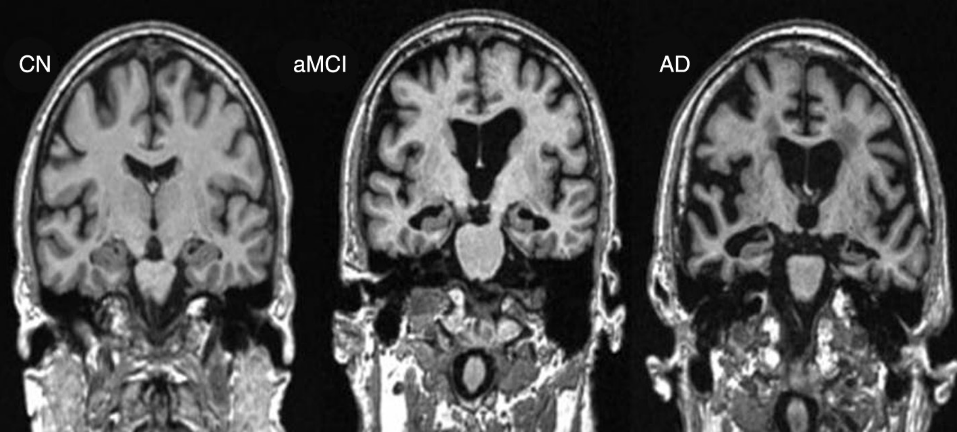
\includegraphics[scale=0.3]{assets/images/mri_brain_antrophy.png}
    \caption{\textbf{Typické odumieranie mozgového tkaniva zachytené magnetickou rezonanciou.} Obrázok zľava, označený ako CN (angl. cognitive normal), reprezentuje kognitívne normálneho jedinca. Obrázok v strede, označený ako aMCI (angl. amnestic mild cognitive impairment) reprezentuje jedinca s miernym kognitívnym poškodením - na obrázku je zreteľný úbytok mozgového tkaniva (šedá farba) najmä v strede mozgu (ale aj na jeho okrajoch) oproti kognitívne normálnemu jedincovi. Posledný obrázok označený ako AD (angl. Alzheimer’s disease) reprezentuje jedinca s Alzheimerovou chorobou - na obrázku je zreteľný značný úbudok mozgového tkaniva. \cite{khan2016biomarkers}
    } 
    \label{fig:mri_brain_antrophy}
\end{figure}

Snímky z pozitrónovej emisnej tomografie (PET) dokážu zachytiť pokles mozgovej aktivity, ktorá je u pacientov s Alzheimerovou chorobou nižšia. Mozgová aktivita odráža úroveň metabolizmu glukózy v mozgu. Na miestach v mozgu, ktoré sú touto chorobou postihnuté, je úroveň metabolizmu glukózy nižšia. Tento jav je znázornený na obrázku \ref{fig:pet}.

\begin{figure}[h!]
    \centering
    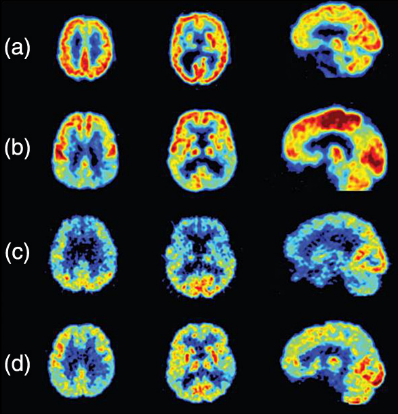
\includegraphics[scale=0.5]{assets/images/pet.png}
    \caption{\textbf{Snímky normálneho mozgu a mozgu postihnutého Alzheimerovou chorobou z pozitrónovej emisnej tomografie (PET).} \cite{khan2016biomarkers}
    Na obrázkoch je viditeľná úroveň metabolizmu glukózy, u pacientov s Alzheimerovou chorobou je táto úroveň nižšia (žltá a modrá farba na obrázkoch).
    (a) Mozog kognitívne zdravého jedinca - vyznačuje sa vyššou mozgovou aktivitou.
    (b) Mozog vyznačujúci symptómy Alzheimerovej choroby - je vidieť nižšiu aktivitu v niektorých častiach mozgu oproti kognitívne zdravému jedincovi.
    (c) Mozog postihnutý frontotemporálnou demenciou (angl. frontotemporal dementia), tiež sa vyznačuje nižšou mozgovou aktivitou.
    (d) Mozog postihnutý Alzheimerovou chorobou.
    } 
    \label{fig:pet}
\end{figure}

% Príklad snímku z MRI je zobrazený na obrázku \ref{fig:mri}.

% \begin{figure}[h!]
% \centering
% 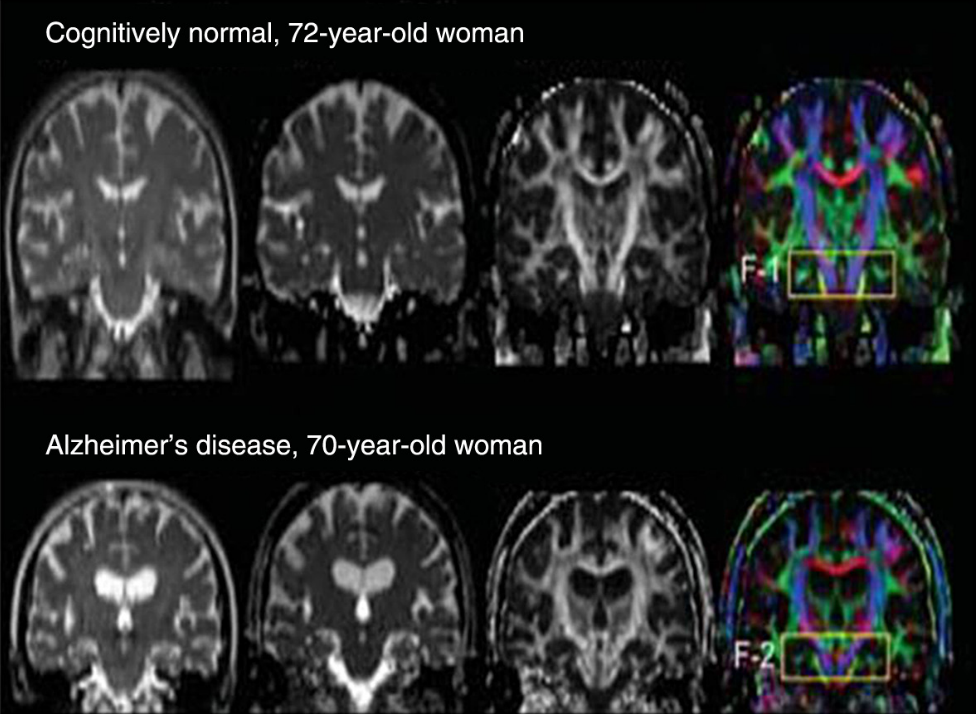
\includegraphics[scale=0.6]{assets/images/mri.png}
% \caption{Zobrazenie difúzneho tenzora (DTI) mozgu pacienta s Alzheimerovou chorobou v porovnaní s kognitívne normálnym jedincom. \cite{khan2016biomarkers} % Obrázok je prevzatý z "Biomarkers in Alzheimer’s Disease", \citeauthor{khan2016biomarkers} \citeyear{khan2016biomarkers}
% }
% \label{fig:mri}
% \end{figure}

\section{Neurónové siete}

Neurónové siete patria medzi obľúbené techniky strojového učenia. Špeciálnou kategóriou sú hlboké neurónové siete (často označované skratkou DNN od angl. deep neural network), ktoré sa oproti obyčajným neurónovým sieťam odlišujú počtom vrstiev. Hlbokým neurónovým sieťam sa doteraz podarilo dosiahnuť v mnohých úlohách výnimočné výsledky, v ktorých častokrát už dokázali prekonať človeka. V našej oblasti obrazových rádiologických dát sa používajú najmä konvolučné neurónové siete.

\citeauthor*{haykin2009neural} \cite{haykin2009neural} definujú neurónovú sieť nasledovne: 
\begin{quote}Neurónová sieť je veľký paralelný distribuovaný procesor tvorený jednoduchými procesorovými jednotkami, ktorý má prirodzený sklon ukladať poznatky a sprístupňovať ich na použitie. Ľudskému mozgu sa podobá v dvoch aspektoch: 
    \begin{enumerate}
        \item Neurónová sieť získava vedomosti zo svojho prostredia prostredníctvom procesu učenia.
        \item Na uchovanie získaných poznatkov sa používajú prepojenia medzi jednotlivými neurónami.
    \end{enumerate}
\end{quote}
Neurónové siete sú teda inšpirované fungovaním mozgu človeka, keďže napodobňujú jeho fungovanie.

\subsection{Neurón} 

Neurón (Obr. \ref{fig:neuron}) je základnou stavebnou jednotkou neurónových sietí. Matematicky sa dá zapísať ako \cite{haykin2009neural}:

\begin{equation}
    y_k = \varphi(b_k + \sum_{j=1}^{m} w_{kj}\cdot x_j)
    \label{eq:neuron}
\end{equation}

Kde:
\begin{itemize}
    \item $x_1, x_2, ... x_m$ sú vstupné signály
    \item $w_{k1}, x_{k2}, ... x_{km}$ sú váhy neurónu $k$
    \item $b_k$ je sklon neurónu $k$
    \item $\varphi(...)$ je aktivačná funkcia
    \item $y_k$ je výsupný signál neurónu $k$
\end{itemize}

Parametrami, ktoré sa počas trénovania neurónovej siete menia sú váhy $w_{kj}$ a sklon $b_{k}$, tieto parametre sú takzvané trénovateľné parametre. Tieto parametre sa upravujú pri spätnej propagácii (angl. backpropagation), kedy sa minimalizuje chybová funkcia (angl. loss function).

V neurónových sieťach s viac vrstvami sa stávajú výstupné signály $y$ neurónov jednej vrstvy vstupom $x$ do ďaľšej.

Aktivačná funkcia zabezpečuje nelinearitu neurónu, medzi najpoužívanejšie aktivačné funkcie patria Sigmoid ($S(x) = \frac{1}{1 + e^x}$), Tanh alebo ReLU ($ReLU(x) = max(0, x)$). Jednotlivé neuróny si môžeme predstaviť ako nelineárne funkcie, ktorých spojením do viac vrstiev dokážu skladať ešte zložitejšie a komplexnejšie funkcie.

\begin{figure}[h!]
    \centering
    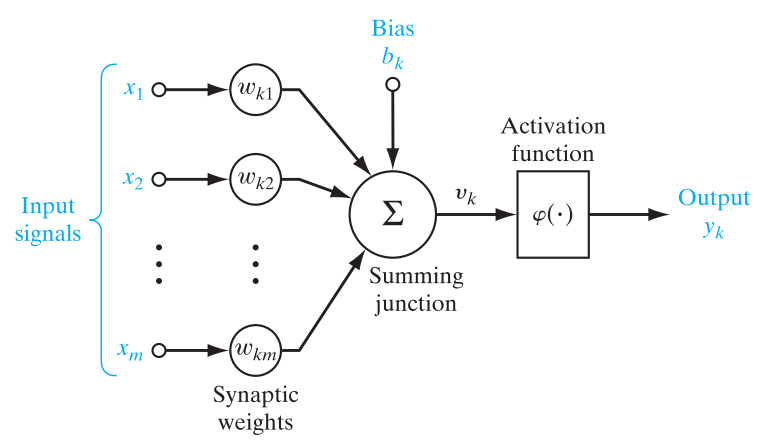
\includegraphics[scale=1]{assets/images/neuron.png}
    \caption{\textbf{Model neurónu.} \cite{haykin2009neural} Neurón sa skladá zo vstupných signálov a váh, ktoré sú na tieto signály aplikované, sklon ($b_k$ - angl. bias) a aktivačnej funkcie, ktorá zapezpečuje nelinearitu. Vzorec \ref{eq:neuron} matematicky popisuje správanie neurónu.} 
    \label{fig:neuron}
\end{figure}

\subsection{Dopredné neurónové siete}

Dopredné neurónové siete (Obr. \ref{fig:ff_nn}) sú jednou z mnoha architektúr neurónových sietí. V dopredných neurónových sieťach výstupný signál z jednej vrsvy nemôže byť vstupným signálom do jej predošlej vrstvy. Signál je prenášaný iba v jednom smere -- dopredu. Dopredné neurónové siete sa môžu skladať z viacerých vrstiev. Základom je vstupná a výstupná vrstva a ľubovolný počet skrytých vrstiev. Ich počet nie je limitovaný, avšak v hlbokých neurónových sieťach (tj. sieťach s veľkým početom skrytých vrstiev) môže nastať problém miznúceho gradientu.

\begin{figure}[h!]
    \centering
    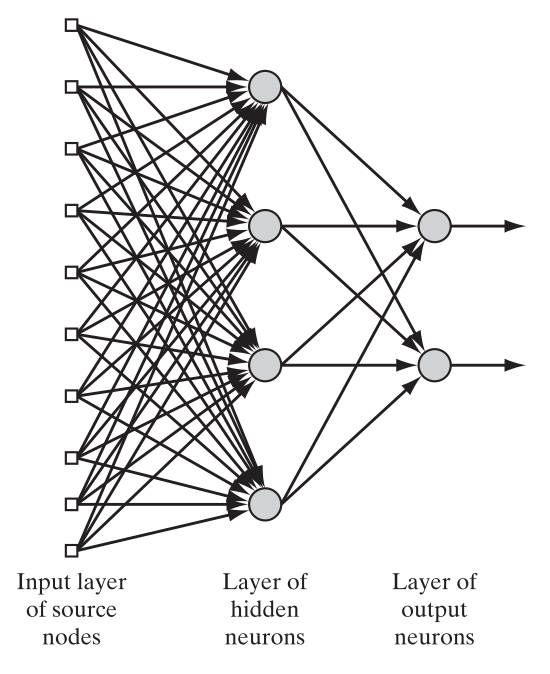
\includegraphics[width=8cm]{assets/images/ff_nn.png}
    \caption{\textbf{Model doprednej neurónovej siete.} \cite{haykin2009neural} Dopredné neurónové siete sa skladajú zo vstupnej vrstvy, skrytých vrstiev a výstupnej vrstvy. Keď hovoríme o počte vrstiev vstupnú vrstvu nepočítame. Neurónová sieť na obrázku má teda dve vrstvy.}
    \label{fig:ff_nn}
\end{figure}

\subsection{Konvolučné neurónové siete}

Konvolučné neurónové siete sa používajú prevažne v doméne obrazových dát. Tieto siete majú schopnosť naučiť sa rozpoznávať špecifické štruktúry/tvary z obrázka. Toto dokážu pomocou takzvaných konvolučných filtrov, ktoré sa v nižších vrstvách naučia rozoznávať jednoduchšie tvary, akými sú napríklad obrysy alebo hrany (Obr. \ref{fig:cnn}). V tých vyšších vrstvách sú to zložitejšie štruktúry akými môžu byť celé objekty v závislosti od typu úlohy na ktorú boli trénované. Ak bola neurónová sieť trénovaná napríklad na klasifikáciu zvierat, môže tým objektom byť pes alebo morča, v prípade ak je úlohou neurónovej siete detekcia Alzheimerovej choroby možu týmito objektami byť niektoré väčšie časti mozgu (napr. hippocampus).

\begin{figure}[h!]
    \centering
    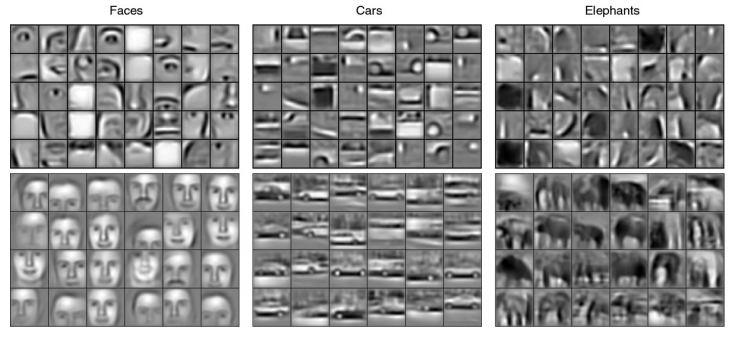
\includegraphics[scale=0.5]{assets/images/cnn.png}
    \caption{
        Vizualizácia druhej (hore) a tretej vrstvy (dole) konvolučných neurónových sietí naučených na špecifické kategórie objektov (tváre, autá a slony). \cite{Lee_Grosse_Ranganath_Ng} Nižšie vrstvy rozoznávajú jednoduchšie štruktúry zatiaľ čo vyššie už dokážu rozonávať aj tie zložitejšie.
    }
    \label{fig:cnn}
\end{figure}

Základnými stavebnými blokmi konvolučných neurónových sietí sú konvolučné vrstvy (angl. convolutional layers) a združovacie vrstvy (angl. pooling layers).

\paragraph{Konvolučné vrstvy}

Pomocou konvolučných vrstiev sa neurónová sieť učí extrahovať črty z obrázka \cite{haykin2009neural}. Konvolúcia prebieha tak, že tzv. jadro (angl. kernel) sa posúva po tzv. mape vlastností (angl. feature map) a matematickými operáciami z pôvodnej mapy vlastností a svojich parametrov vytvára novú mapu vlastností. Tieto parametre sú trénovateľné, čo umožňuje sa každému jadru naučiť urćitú črtu - napr. hranu. Konvolučná vrstva tiež dokáže znižovať kompexitu modelu (a teda aj počet jeho parametrov) jej hyper parametrami (angl: stride, padding, depth).

\paragraph{Združovacie vrstvy}

Cieľom združovacích vrstiev je postupne znižovať dimenzionalitu dát, tým znižovať počet počet parametrov modelu, a teda aj jeho komplexitu \cite{o2015introduction}. Najčastejšie sa používajú vrstvy združujúce maximom (angl. max-pooling), ale existujú aj vrsvy združujúce priemerom či súčtom.

\begin{figure}[h!]
    \centering
    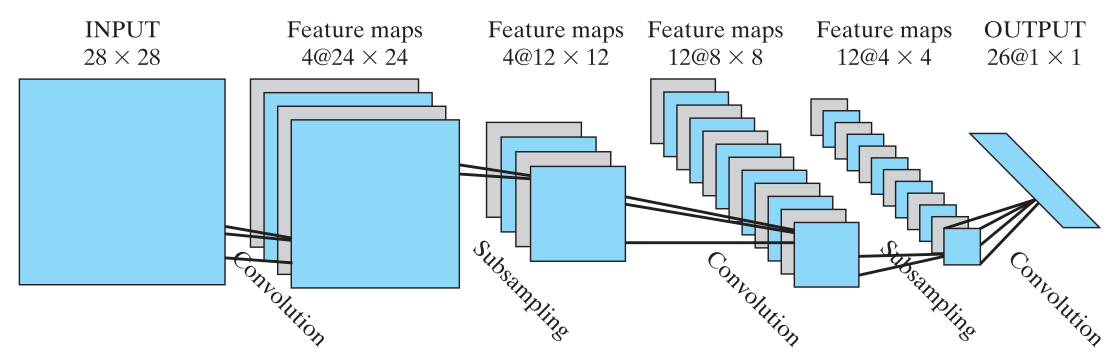
\includegraphics[width=12cm]{assets/images/conv_net_architecture.png}
    \caption{\textbf{Príklad architektúry konvolučnej neurónovej siete. \cite{haykin2009neural}} V tejto achitektúre neurónovej siete sa používajú tri konvolučné vrstvy (označené ako \textit{convolution}) a dve združovacie vrstvy (označené ako \textit{subsampling}). Môžeme si všimnúť, že konvolučné vrstvy postupne pridávajú mapy vlastností (tiež ozačované ako: angl. ''volumes'') a tiež mierne znižujú ich veľkosť. Združovacie vrstvy zasa výrazne znižujú ich veľkosť (až o polovicu) a tým aj počet parametrov v neurónovej sieti.}
    \label{fig:conv_net_architecture}
\end{figure}

\subsection{Architektúry konvolučných neurónových sietí}

Architektúra neurónovej siete hovorí o tom, ako neurónová sieť vyzerá - koľko má vrstiev, z akých vrstiev sa skladá (konvolučné, združovacie, husté), koľko filtrov je v jednotlivých vrstvách a pod. Nie každá architektúra je vhodná na každý problém. Ak je problém jednoduchý, môže byť použitie veľmi hlbokej neurónovej siete zbytočné. Taktiež, jednoduchšia architektúra potrebuje menej výpočtových zdrojov na natrénovanie a je odolnejšia voči pretrénovaniu. Spomeniem niekoľko najznámejších architektúr, ktoré sú používané najmä pri klasifikácii obrazových dát.

\begin{itemize}
    \item VGG \cite{simonyan2014very} - hlboká neurónová sieť, so 16 alebo s 19 vrstvami. Skladá sa s konvolučných a združovacích vrstiev.
    \item ResNET \cite{he2016deep} - hlboká neurónová sieť skladajúca sa z reziduálnych blokov. Reziduálne bloky obsahujú skracovacie spojenia, "skratky" (angl. shortcut connections) ako nástroj na zabránenie miznúcemu a explodujúcemu gradientu. Táto architektúra bola navrhnutá s 20, 32, 44, 56, 110 a 1202 vrstvami.
    \item Inception (GoogLeNet) \cite{szegedy20s15going} - hlboká neurónová sieť skladajúca sa s inception blokov. Každý blok robí niekoľko rôznych konvolúcii zo vstupu daného bloku, ktoré sú následne spojené v združovacom bloku.
\end{itemize}

Taktiež existuje niekoľko ďaľších vylepšení Inception architektúry (Inception v1 až v4), dokonca aj kombinácia s architektúrou ResNet.

\begin{figure}[h!]
    \centering
    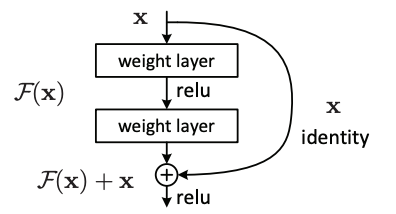
\includegraphics[scale=0.6]{assets/images/residual_block.png}
    \caption{Reziduálny blok v architektúre ResNET. Informácia z predhádzajúceho bloku je súčasťou výstupu aktuálneho bloku pomocou skracovacieho spojenia. \cite{he2016deep}}
    \label{fig:residual_block}
\end{figure}

\subsection{Interpretovanie neurónovej siete}

\citeauthor{montavon2018methods} (\citeyear{montavon2018methods}) definujú interpretovanie ako mapovanie abstraktného konceptu (napríklad predikovanej triedy) do domény, ktorej človek dokáže porozumieť. Ako príklad domény, ktorá je interpretovateľná uvádzajú obrázky (pole pixelov) alebo text (sekvencia slov) \cite{montavon2018methods}. Medzi domény, ktoré nie sú interpretovateľné zaraďujú napríklad latentné vektorové reprezentácie slov (angl. word embeddings) alebo iné abstraktné vektorové reprezentácie \cite{montavon2018methods}.
Na rozdiel od vstupných dát do neurónovej siete, ktoré sú zvyčajne interpretovatelné, neuróny na výstupnej vrstve a v skrytých vrstvách sú abstraktné a vyžadujú dodatočné úsilie na ich interpretovanie. Jedným zo spôsobov interpretovania týchto neurónov je maximalizácia aktivácie (angl. activation maximization).

\paragraph{Maximalizácia aktivácie (angl. Activation maximization)}
Maximalizácia aktivácie je metóda na nájdenie takého vstupného prototypu, ktorý vyprodukuje najväčšiu mieru aktivácie pre zvolený neurón (zvyčajne je to neurón hľadanej triedy na najvyššej vrstvy). 
% Takýto vstupný prototyp je nájdený optimalizovaním nasledovnej funkcie pomocou poklesu gradientu (angl. gradient descent).
Takýto vstupný prototyp je nájdený tak, že neurónovej sieti je daný na vstup neutrálny obrázok, ktorý v danej doméne nereprezentuje žiadnu triedu (zvyčajne sa jedná o šedý obrázok) a je optimalizovaná funkcia maximalizácie aktivácie pomocou poklesu gradientu \cite{montavon2018methods} (angl. gradient descent). Pri aplikovaní tejto metódy na obrazové dáta výsledné prototypy vyzerajú tak ako na obrázku \ref{fig:activation_maximization}.

\begin{figure}[h!]
\centering
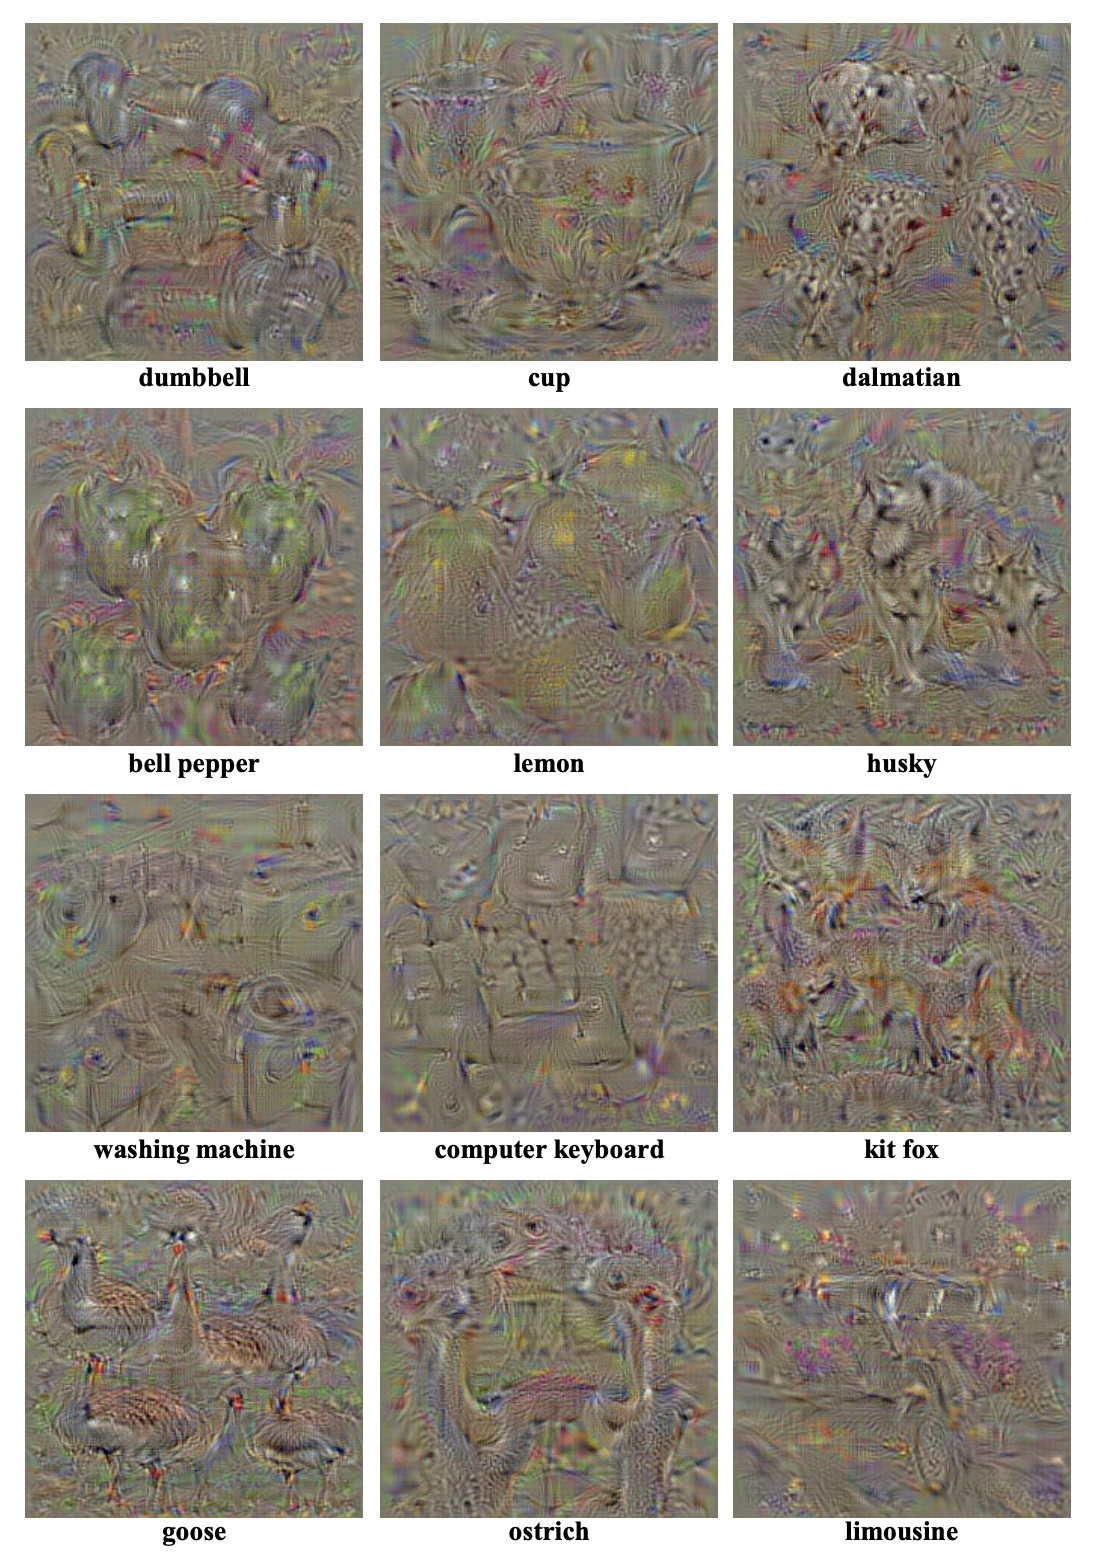
\includegraphics[scale=0.6]{assets/images/activation_maximization.png}
\caption{\textbf{Maximalizácia aktivácie aplikovaná na obrazové dáta. \cite{simonyan2013deep}} Výsledné vzorové prototypy pre jednotlivé triedy nevyzerajú prirodzene, sú prevažne šedé s farebnými črtami objektov. Tieto vzorové prototypy nereprezentujú príklady vstupov ''z reálneho sveta'' ale ideálne vstupy pre jednotlivé triedy. Takéto vstupy nerónová sieť bežne nedostane.
}
\label{fig:activation_maximization}
\end{figure}

\paragraph{Maximalizácia aktivácie s expertom}
Na získanie realistickejších prototypov (prototypov, ktoré sa viac podobajú vstupným dátam) $l_2$-regularizácia (používaná v maximalizácii aktivácie) je nahradená takzvaným ``expertom``, ktorý sa snaží naučiť distribúciu hľadanej triedy \cite{montavon2018methods}. Oproti $l_2$-regularizácii, ktorá hľadá vstup maximalizujúci pravdepodobnosť triedy, expert hľadá taký vstup, ktorý je najpravdepodobnejší pre zvolenú triedu. Ako ``expert`` môže byť použitý napríklad Gaussian RBM (angl. Restricted Boltzmann machine) \cite{montavon2018methods}.
% TODO: niesom si isty, opytat sa "naučiť distribúciu hľadanej triedy", a ta posledna veta ci citovat prehladovy clanok alebo clanok z prehladoveho clanku ktory som ani necital

% AM in code space, doplnit? Tam sa pouzivaju tie GAN...
% TODO: AM in code space
% k tomu je velmi prijemny obrazok tuto http://iphome.hhi.de/samek/pdf/DTUSummerSchool2017_1.pdf

\subsection{Vysvetľovanie predikcie neurónovej siete}

\citeauthor{montavon2018methods} (\citeyear{montavon2018methods}) definujú vysvetľovanie ako kolekciu vlastností dát, ktoré sú z interpretovateľnej domény, ktoré prispeli k výslednému rozhodnutiu (napr. zaradenie do určitej triedy - klasifikácia) pre určité pozorovanie \cite{montavon2018methods}. Rozdiel oproti interpretovaniu teda je, že pri interpretovaní hľadáme vzorový prototyp (vzorové pozorovanie) pre zvolenú triedu, zatiaľ čo pri vysvetľovaní sa snažíme zistiť prečo, a teda ktoré z vlastností vstupu najviac prispeli (tj. sú najviac relevantné) k výslednej predikcii neurónovej siete (napr. zaradenie pozorovania do určitej triedy). 

Niektoré metódy vysvetľovania fungujú na základe zakrývania častí obrázka a sledovaním zmeny predikcie predikovanej triedy -- perturbačné metódy, iné zasa na základe spätného šírenia (angl. backpropagation) -- napr. LRP, analýza senzitivity.

Každá z metód má svoje výhody a nevýhody, napríklad výhodou perturbačných metód je, že môžu byť použité na akýkoľvek model, keďže jediné čo potrebujú je výstup (predikciu) z modelu. Ich nevýhodou však je, že sú pomalé. Niektoré z metód vysvetľovania bližšie opíšeme v tejto sekcii.

\subsubsection{Analýza senzitivity}

Analýza senzitivity slúži na vysvetľovanie predikcie neurónovej siete. Táto metóda identifikuje, ktoré z vlastností vstupného pozorovania najviac prispievajú výslednej predikcii. Najviac dôležité sú také vlastnosti, ktorých zmenou sa najvýraznejšie zmení výsledná predikcia. Na takéto vlastnosti je výsledná predikcia najviac citlivá \cite{montavon2018methods}.

Výsledok analýzy senzitivity znázornený v tepelnej mape (angl. heatmap) je zobrazený na obrázku \ref{fig:sensitivity_analysis}. Analýza senzitivity zachytáva teda vlastnosti vstupného pozorovania, ktoré k výslednej predikcii prispievajú pozitívne aj negatívne (napr. zmenením určitej vlastnosti vstupu sa výrazne zníži zaradenie do danej triedy). Na výslednej tepelnej mape vlastnosti, ktoré k výslednej predikcii prispievajú pozitívne, a vlastnosti, ktoré k výslednej predikcii prispievajú negatívne (proti), nevieme rozlíšiť. Vieme len, že zmenením danej vlastnosti výrazne ovplyvníme predikciu.

\begin{figure}[h!]
\centering
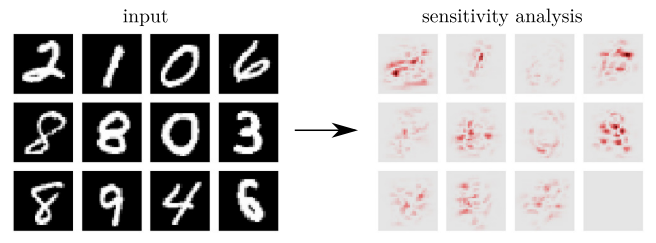
\includegraphics[scale=0.5]{assets/images/sensitivity_analysis.png}
\caption{\textbf{Analýza senzitivity aplikovaná na konvolučnú neurónovú sieť trénovanú na dátovej sade MNIST. \cite{montavon2018methods}} Červenou farbou sú zobrazené miesta ktoré najviac prispievajú, či už pre alebo proti, výslednej predikcii. Čím je červená farba výraznejšia, tým viac je výsledok senzitívny na zmenu daného pixela.}
\label{fig:sensitivity_analysis}
\end{figure}

\subsubsection{LRP (angl. layer-wiser relevance propagation)}

Metóda vrstvami propagovanej relevancie, ďalej len LRP (angl. layer-wise relevance propagation), sa od analýzy senzitivity odlišuje tým, že vo výslednej tepelnej mape dokáže odlíšiť vlastnosti, ktoré prispeli pozitívne alebo negatívne k výslednej predikcii (v zázislosti od použitých parametrov $\alpha$ a $\beta$).

Táto technika funguje tak, že vstupný obrázok dopredným šírením ''prejde'' neurónovou sieťou, pričom sú zozbierané aktivácie neurónov v jednotlivých vrstvách. Následne je neurónovou sieťou spätným šírením propagované skóre z výstupu neurónovej siete v podobe relevancie až k vstupnému obrázku. 

Nasledovné vzorce \ref{eq:lrp_1}, \ref{eq:lrp_2}, \ref{eq:lrp_3} \cite{montavon2018methods} vyjadrujú spôsob výpočtu propagovanej relevancie medzi vrstvami. $j$ a $k$ sú jednotlivé vrstvy, pričom $k$ je vrstva, z ktorej je relevancia $R$ propagovaná. Parametre $\alpha$ a $\beta$ upravujú, koľko pozitívnej ($\alpha$) alebo negatívnej ($\beta$) relevancie je vytvorenej počas fázy spätného šírenia relevancie. Pri ich nastavovaní musí platiť, že $\alpha - \beta = 1$ a zároveň $\beta \geq 0$. Súčet pozitívnej a negatívnej relevancie je však medzi vrstvami vždy rovnaký \cite{montavon2018methods}, výsledok použitia rôznych hodnôt $\alpha$ a $\beta$ je znázornený na obrázku \ref{fig:lrp}. $R_{j\leftarrow k}^{+}$ (Obr. \ref{eq:lrp_1}) a $R_{j\leftarrow k}^{-}$ (Obr. \ref{eq:lrp_3}) vyjadrujú množstvo pozitívnej ($+$), resp. negatívnej ($-$) relevancie propagovanej z vrstvy $k$ do vrstvy $j$. $a_j$ je aktivácia neurónu, na ktorý je propagovaná relevancia.

% Option 1
% \begin{equation}
%     R_{j}=\sum_{k}^{}\frac{a_j w_{j k}^+}{\sum_{j}^{} a_j w_{j k}^+}\alpha R_k + \sum_{k}^{}\frac{a_j w_{j k}^-}{\sum_{j}^{} a_j w_{j k}^-}\beta R_k
%     \label{eq:lrp}
% \end{equation}

% Option 2
\begin{equation} 
    R_{j\leftarrow k}^{+} = \frac{a_j w_{j k}^+}{\sum_{j}^{} a_j w_{j k}^+}
    \label{eq:lrp_1}
\end{equation}
\begin{equation} 
    R_{j\leftarrow k}^{-} = \frac{a_j w_{j k}^-}{\sum_{j}^{} a_j w_{j k}^-}
    \label{eq:lrp_2}
\end{equation}
\begin{equation} 
    R_{j}=\sum_{k}^{} \left ( \alpha R_{j\leftarrow k}^{+} - \beta R_{j\leftarrow k}^{-} \right ) R_k
    \label{eq:lrp_3}
\end{equation}

\begin{figure}[h!]
\centering
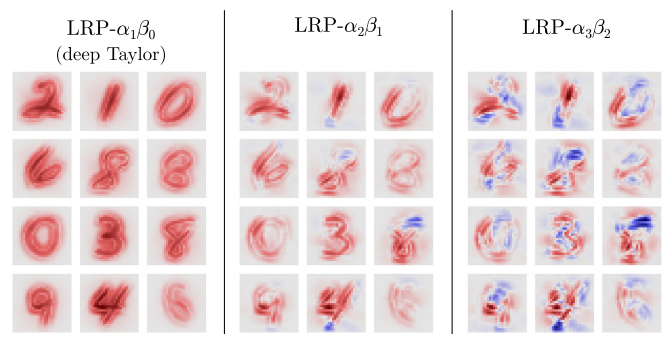
\includegraphics[scale=0.5]{assets/images/lrp.png}
\caption{\textbf{Výsledné vysvetlenie (v podobe tepelnej mapy) vytvorené použitím LRP s rôznymi hodnotami $\alpha$ a $\beta$ na dátovej sade MNIST. \cite{montavon2018methods}} Pozitívna relevancia je zobrazená červenou farbou \cite{montavon2018methods}. Negatívna relevancia je zobrazená modrou farbou \cite{montavon2018methods}. V prípade, že použijeme $\alpha = 1$ a $\beta = 0$ strácame informáciu o tom, ktoré pixely negatívne (tj. sú proti výslednej predikcii) prispeli k výslednej predikcii (a opačne).}
\label{fig:lrp}
\end{figure}

Výhodou LRP oproti iným metódam, ako napríklad dekonvolúcii je, že vysvetlenie (výsledná tepelná mapa) vytvorené technikou LRP je pre rôzne obrázky vždy rôzne \cite{Muller_Samek_Montavon_Lapuschkin_Arras}. Naopak, pri dekonvolúcii je vysvetlenie vždy rovnaké pokiaľ v architektúre neurónovej siete neboli použité združovacie vrstvy (angl. pooling layers) \cite{Muller_Samek_Montavon_Lapuschkin_Arras}. Ďaľším rozdielom je (aj oproti analýze senzitivity), že vo výslednom vysvetlení LRP rozlišuje, ktoré vlastnosti pozitívne alebo negatívne prispeli k negatívnej predikcii.

% TODO: vysvetlit dekonvoluciu???

\subsubsection{RISE - Randomized Input Sampling for Explanation \label{sec:rise}}

Túto metódu môžeme zaradiť medzi perturbačné metódy, keďže je tiež založená na zakrývaní jednotlivých častí obrazu a sledovaním zmeny výslednej predikcie modelu. Už z názvu modelu \textit{(Randomized Input Sampling for Explanation)} je zrejmé, že táto metóda využíva náhodu na zakrývanie jednotlivých častí vstupného obrazu. Vstupný obraz je prekrytý náhodou maskou, ktorá je vytvorená nasledovne \cite{petsiuk2018rise}:

\begin{itemize}
    \item Je vytvorená náhodná binárna (tj. iba z bielej a čiernej farby) maska o malej veľkosti (napríklad 8px x 8px).
    \item Táto maska je zväčšená (angl. upsampled) pomocou bilineárnej interpolácie \cite{petsiuk2018rise} (angl. bilinear interpolation) na veľkosť ktorá je mierne väčšia ako veľkosť obrázka s ktorým bude prekrytá (kvôli oreznávaniu). Tým sa zníži jej kvalita a ostré hrany medzi bielymi a čiernymi časťami sa zjemnia. Masky už teda nie sú binárne.
    \item Z masky je náhodne vyrezaná náhodná čast o veľkosť prekrývaného obrázka.
\end{itemize}

% To address these issues we first sample smaller binary masks and then upsample them to
% larger resolution using bilinear interpolation. Bilinear upsampling does not introduce sharp edges in I?Mi as well as results in a smooth importance map S.

Toto sa opakuje $N$ krát. Výsledná tepelná mapa je vypočítaná ako vážený priemer všetkých vygenerovaných masiek, kde váhy sú skóre (pravdepodobnosť predikovanej triedy) z modelu. Tento proces je zobrazený na obrázku \ref{fig:rise_architecture}.

\begin{figure}[h!]
    \centering
    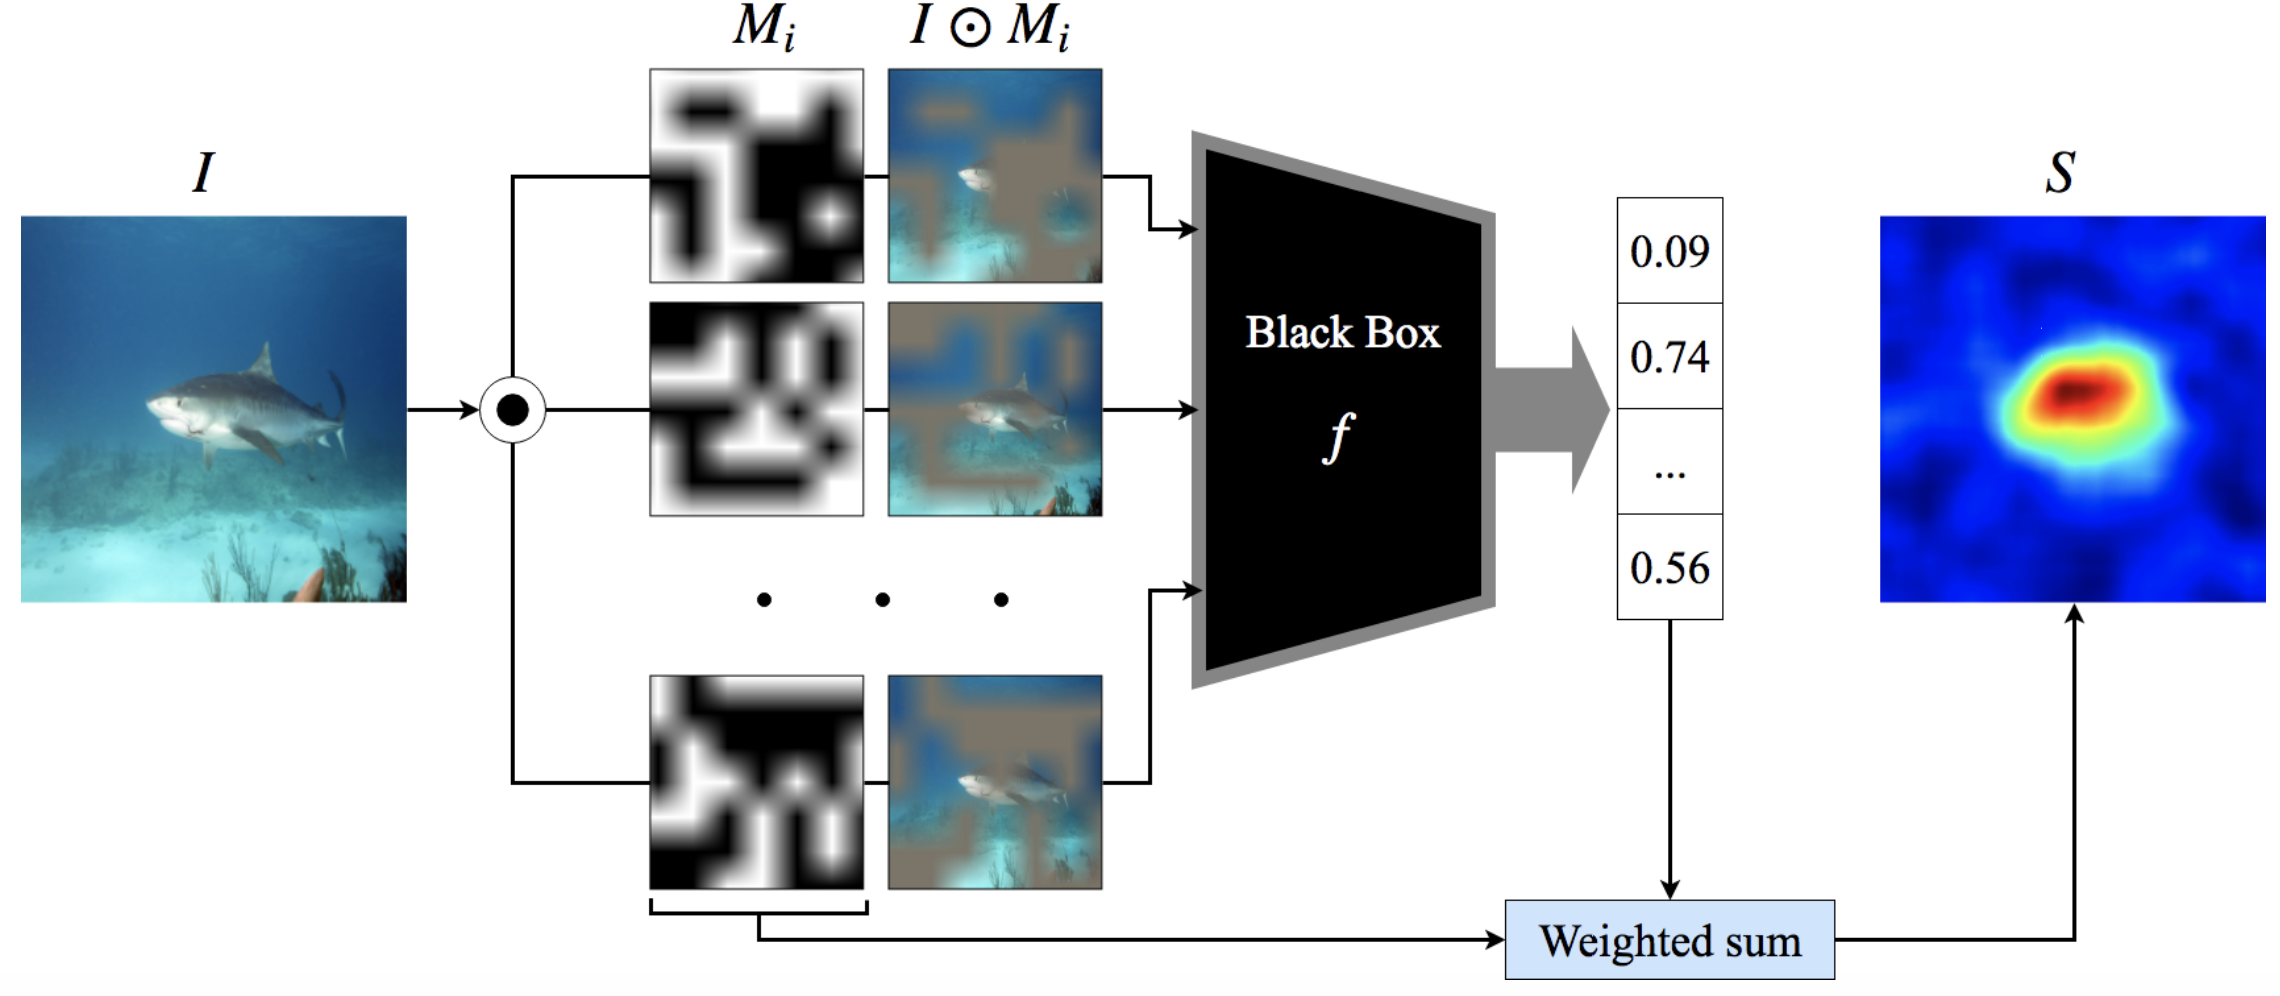
\includegraphics[scale=0.35]{assets/images/rise_architecture.png}
    \caption{Metóda \textit{RISE}. \cite{petsiuk2018rise} Vygenerované masky nahrádzajú vstupný obrázok na, ktorý sú aplikované. Z výstupných predikcii jednotlivých masiek je nakoniec vypočítaná tepelná mapa.}
    \label{fig:rise_architecture}
\end{figure}

Autori porovnali túto metódu s metódami \textit{GradCAM} (\citeauthor*{selvaraju2017grad} \citeyear{selvaraju2017grad}) \cite{selvaraju2017grad} a \textit{LIME} (\citeauthor*{ribeiro2016should} \citeyear{ribeiro2016should}) \cite{ribeiro2016should}. Metóda \textit{RISE} si oproti týmto dvom metódam počínala lepšie (Obr. \ref{fig:rise_results}). Vykonali niekoľko experimentov, v ktorých porovnali architektúry neurónových sietí \textit{ResNet50} (\citeauthor*{he2016deep} \citeyear{he2016deep}) \cite{he2016deep} a \textit{VGG16} (\citeauthor{simonyan2014very} \citeyear{simonyan2014very}) \cite{simonyan2014very} natrénované na dátových sadách PASCAL VOC07 (\citeauthor*{everingham2010pascal} \citeyear{everingham2010pascal}) \cite{everingham2010pascal} a MSCOCO2014 (\citeauthor*{lin2014microsoft} \citeyear{lin2014microsoft}) \cite{lin2014microsoft}. Sledovali metriky \textit{insertion} a \textit{deletion} (Obr. \ref{fig:rise_results}). Metrika \textit{insertion} je vyjadrená ako plocha pod krivkou (AUC) funkcie $y = f(x)$, kde $y$ je istota predikcie a $x$ je počet pridaných najdôležijetších pixelov, dôležitosť pixelov je určená metódou vysvetľovania predikcie neurónovej siete a môže byť zobrazené pomocou tepelnej mapy. Metrika \textit{deletion} naopak odoberá najdôležitejšie pixely z obrázka.

Výhodou tejto metódy je, že oproti bežným perturbačným metódam je výrazne rýchlejšia.

\begin{figure}[h!]
    \centering
    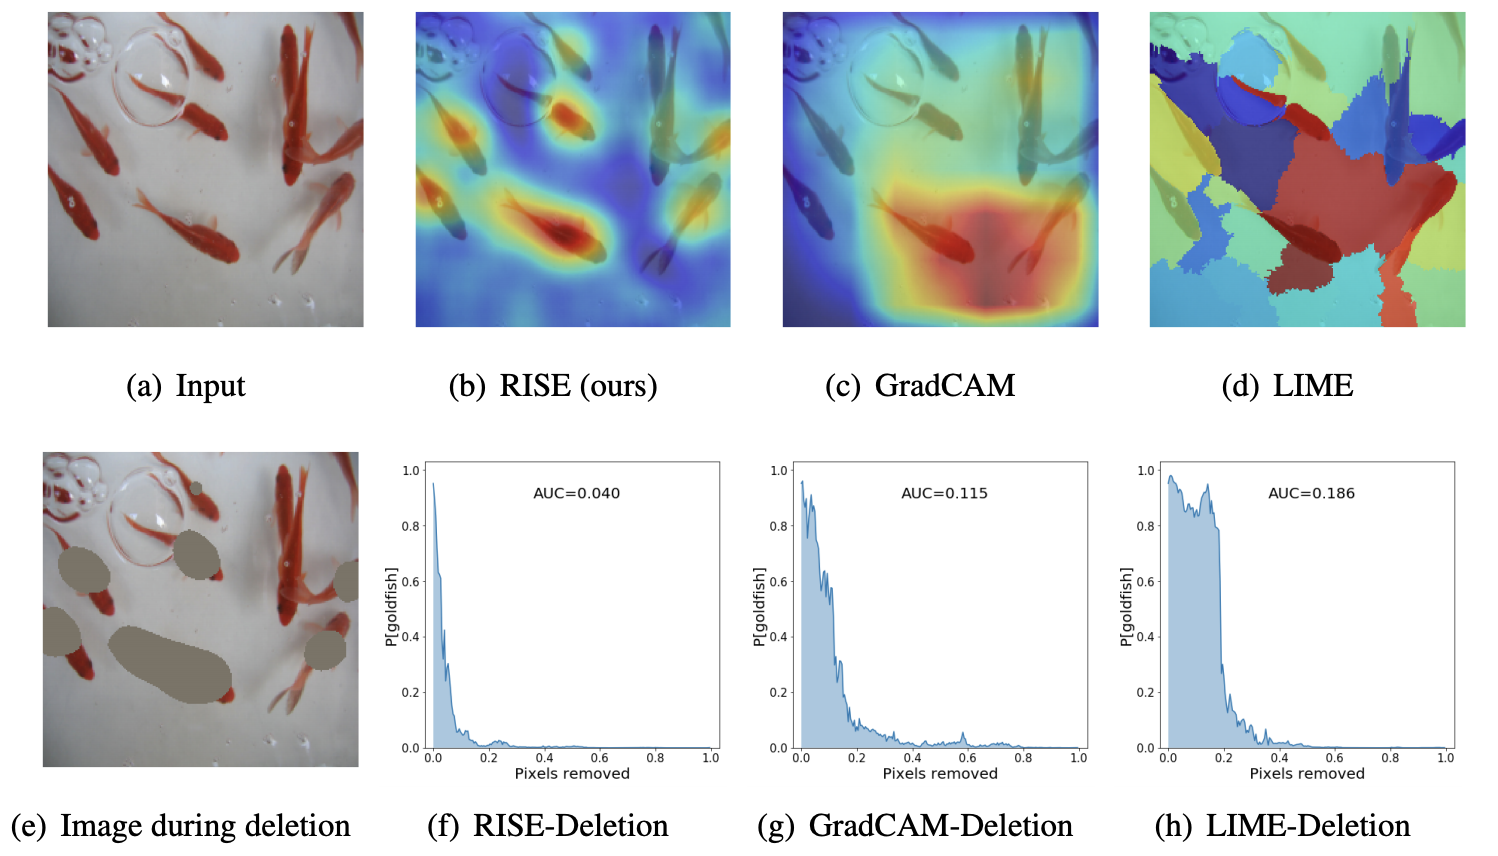
\includegraphics[scale=0.5]{assets/images/rise_results.png}
    \caption{Porovnanie metódy \textit{RISE} s \textit{GradCAM} alebo \textit{LIME}. \cite{petsiuk2018rise} V prvom riadku sú tepelné mapy jednotlivých metód pre vstup. V druhom riadku je znázornená porovnávaná metrika \textit{deletion}. Táto metrika sleduje vzťah medzi odobratím najdôležijetších pixelov a výslednou predikciou modelu. Je vyčíslená pomocou výpočtu plochy pod krivkou (AUC). Na grafoch si môžeme všimnúť, že metóda \textit{RISE} potrebuje odobrať menej pixelov na to aby klesla pravdepodobnosť predikovanej triedy. To znamená, že tepelná mapa (metódy \textit{RISE} oproti ostatným metódam) lepšie zaznamenáva dôležité pixely pre predikovanú triedu.}
    \label{fig:rise_results}
\end{figure}

\section{Využitie neurónových sietí pri odhaľovaní Alzheimerovej choroby \label{sec:nn_ad_prediction}}

Neurónovým sieťam sa doposiaľ podarilo dosiahnuť veľmi dobré výsledky pri odhaľovaní Alzhemiemerovej choroby. Ako vstup používajú rádiologické snímky ako sú z MRI či PET. Tieto rádiologické ukazovateľe sme bližšie popísali v sekcii \ref{sec:neoroimaging_biomarkers}. Okrem rádiolgických snímkov môžu byť vstupom do neurónovej siete demografické údaje o pacientovi, či výstupy z rôznych klinických alebo kongitívnych testov. Takéto údaje o pacientoch obsahuje populárna dátová množina \textit{ADNI-1} \cite{ADNI}.

Neurónové siete natrénované na predikciu Alzheimerovej choroby sa líša najmä v:
\begin{itemize}
    \item \textbf{predspracovaní} - vstupné dáta sú zmenšené/zväčšené rôznymi algorimami na rôzne veľkosti, častokrát sa z rádiologických snímkov odstraňuje lebka
    \item \textbf{type vstupných dát} - môžu to byť rádiologické snímky (MRI, PET), vlasté črty extrahované z rádiologických snímkov (MRI, PET), alebo kombinácia takýcho snímkov/čŕt, s inými, napríklad demografickými údajmi
    \item \textbf{architektúre} - môžu to byť konvolučné siete s 2D konvolúciami (v prípade, že sa používa iba časť rádiologickej snímky, alebo vlastné črty) alebo 3D konvolúciami (ak je vstup celý rádiologický snímok, angl. "full volume"), alebo iné architektúry ako ResNET (reziduálne neurónové suete) alebo VGG
    \item \textbf{ako boli natrénované} - pri niektorých neurónových sieťach autori využili učenie prenosom (angl. transfer learning) a rôzne spôsoby augmentácie vstupus
\end{itemize}

Ako príklad 3D konvolučnej neurónovej siete uvediem neurónovú sieť od \citeauthor*{esmaeilzadeh2018end} s presnosťou \textbf{94.1\%} (a s $F_2$ skóre 0.93) na populárnej dátovej množine s názvom \textit{ADNI-1} (Obr. \ref{fig:ad_cnn_architecture}). Tento výsledok dosiahli v úlohe klasifikácie iba do CN a AD (bez MCI). Vstupom do tejto neurónovej siete boli snímky z magnetickej rezonancie (MRI) ale aj demografické informácie akými sú napríklad vek alebo pohlavie. Autor avšak nereportuje úspešnosť modelu, ktorý bol natrénovaný iba z obrazových dát, táto úspešnosť by bola pravdepodobne o niečo nižšia.

\begin{figure}[h!]
    \centering
    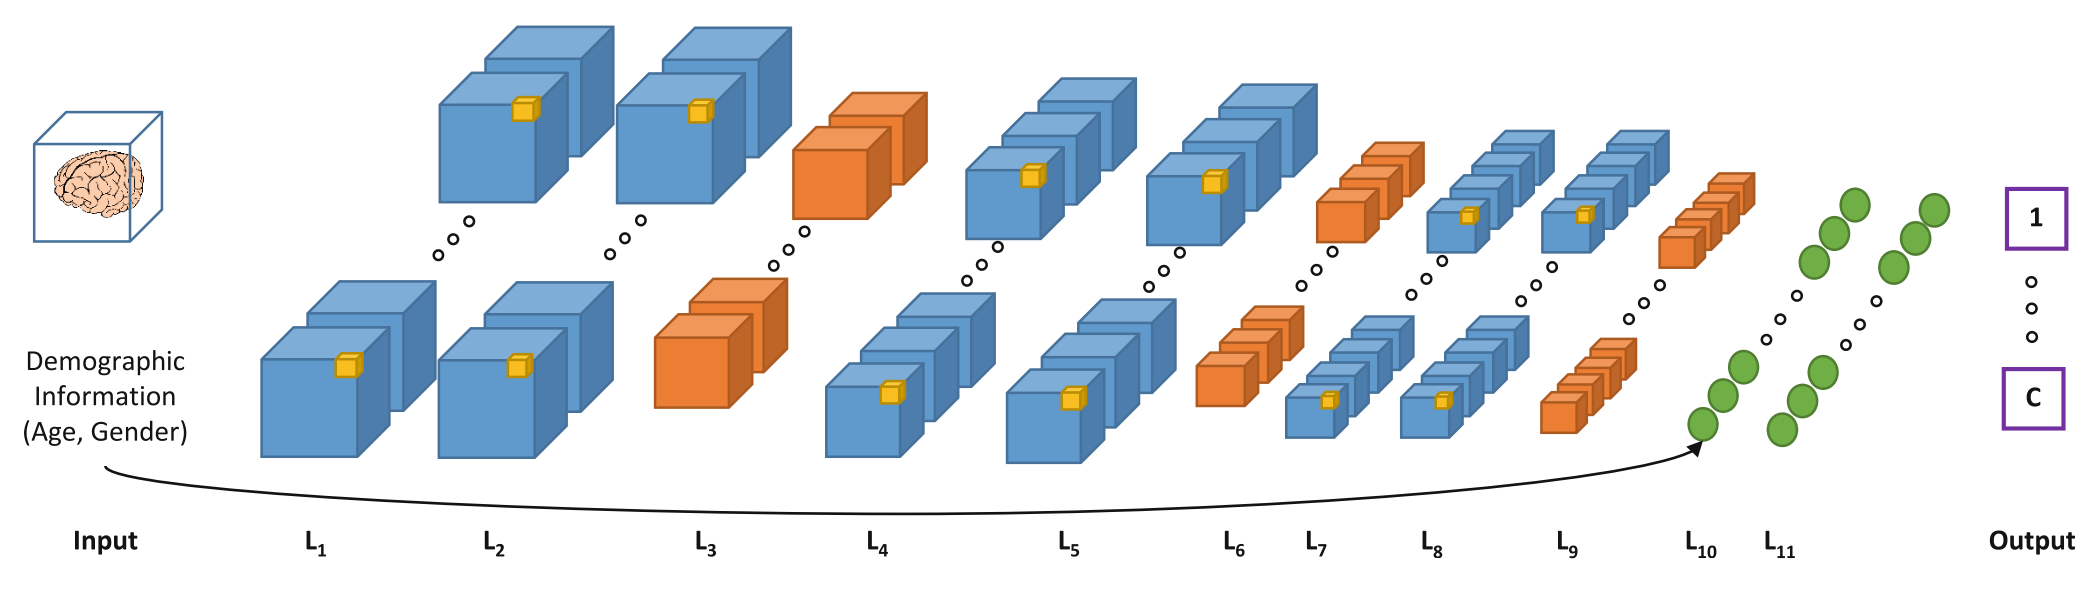
\includegraphics[scale=0.35]{assets/images/ad_cnn_architecture.png}
    \caption{Architektúra konvolučnej neurónovej siete použitej pri detekcii Alzheimerovej choroby. \cite{esmaeilzadeh2018end} Modré kocky sú konvolučné vrstvy, oranžové kocky sú \textit{max-pooling} vrstvy, posledné dve (zelené) vrstvy sú plne prepojené vrstvy. Môžeme si všimnúť, že do posledných dvoch plne prepojených vrstiev okrem obrazových dát vstupujú aj informácie o veku a pohlaví.}
    \label{fig:ad_cnn_architecture}
\end{figure}

V prípade klasifikácie do všetkých troch tried - CN, MCI a AD autori tejto práce dosiahli horšie výsledky oproti binárnej klasifikácii. Ich model dokázal správne zaradiť pacienta s presnosťou \textbf{61.1\%} (a s $F_2$ skóre 0.62) \cite{esmaeilzadeh2018end}. Pri dosiahnutí tohto výsledku použili tzv. učenie s prenosom (angl. transfer learning), ktoré im zlepšilo úspešnosť modelu až o 5.1\% z pôvodných 54\%. Model, z ktorého učili prenosom je už skôršie spomínaný model na binárnu klasifikáciu pacientov s Alzheimerovou chorobou.

Autori experimentovali trénovaním dvoch rôznych modelov, jedného jednoduchšieho a druhého zložitejšieho. Lepší bol jednoduchší model, pretože nebol tak náchylný na pretrénovanie. V týchto modeloch použili dropout, $l_2$ regularizáciu a augmentované dáta (obrázky otočili po osi x). Tieto ''vylepšenia'' pridávali postupne a sledovali rozdiel v úspešnosti modelu, každé jedno z týchto vylepšení výrazne zlepšilo úspešnosť modelu. V kroku predspracovania dát odstránili z obrázkov také časti, ktoré nepredstavovali tkanivo mozgu (napr. lebka) technikou s názvom BET (\citeauthor*{smith2002fast} \citeyear{smith2002fast}) \cite{smith2002fast}, pretože z nich sa Alzheimerova choroba nedá diagnostikovať.

Niektoré práce (\citeauthor*{suk2016deep} \citeyear{suk2016deep}) sa zaoberali dokonca klasifikáciou do štyroch tried: AD, CN, pMCI (angl. progressive MCI - pacienti ktorí pokročili k AD do 18 mesiacov), sMCI (angl. stable MC - pacienti ktorí nepokročili k AD do 18 mesiacov). Táto úloha je samozrejme náročnejšia, najlepší model v tomto prípade dosahoval presnosť 53.72\% \cite{suk2016deep}. V prípade binárnej klasifikácie (AD vs CN) sa autorom podarilo dosiahnuť presnosť až \textbf{95.09}\%, oproti \citeauthor*{esmaeilzadeh2018end} však použili aj rádiologické snímky z PET. Táto práca sa ďalej vyznačuje adaptívnou selekciou čŕt, vďaka ktorej sa autorom podarilo dosiahnuť tak dobré výsledky. V tejto práci autori taktiež vykonali odstránenie lebky zo vstupných snímkov počas fázy predspracovania.

Učenia prenosom (angl. transfer learning) je veľmi dobrým spôsobom na zrýchlenie trénovania a zlepšenie úspešnosti modelu. \citeauthor*{hosseini2016alzheimer} využili učenie prenosom a to tak, že najskôr netrénovali 3D konvolučný autoenkodér, ktorý mal za úlohy rekonštruovať vstup - tj. vstupný radiologický snímok. Z tohto autoenkodéra zobrali jednu jeho časť - enkodér za ktorý dali konvolučné vrstvy, ktoré dotrénovali na detekciu Alzheimerovej choroby. Enkodér teda slúžíl na ektrakciu čŕt.

Neurónové siete sa v niektorých prácach používajú v kombinácii s inými algoritmami strojového učenia. \citeauthor*{suk2017deep} použili kombináciu riedkych regresných modelov (angl. sparse regression models) a 2D konvolučnej neurónovej siete, kde výstupy z týchto regresiných modelov slúžili ako vstup do neurónovej siete.

% https://pubmed.ncbi.nlm.nih.gov/28167394/

\subsection{Vysvetľovanie rozhodnutí neurónových sietí detegujúcich Alzheimerovu chorobu \label{sec:ad_nn_explanation}}

Existujúce práce sa už zaoberali metódami vysvetľovania rozhodnutí neurónových sietí detekujúcich Alzheimerovu chorobu. \citeauthor{bohle2019layer} \citeyear{bohle2019layer} uviedli možnosti analýzy rozhodnutí za účelom ich vysvetľovania. Konkrétne sa zaoberali metódami vrstvami propagovanej relevancie (LRP) a vedenou spätnou propagáciou (angl. guided backpropagation). Uvádzajú LRP ako metódu na vysvetľovanie invididuálnych rozhodnutí neurónovej siete kde naopak vedenú spätnú propagáciu ako metódu na zistenie oblastí, na ktoré je neurónová sieť senzitívna. Tieto metódy skúmali porovnávaním priemerov tepelných máp (angl. heatmaps) všetkých pozorovaní v predikovaných triedach (2 - AD, HC). Taktiež porovnávali priemerné tepelné mapy pozorovaní podľa spôsobu zaradenia výslednej predikcie (4 - true positive, true negative, false positive, false negative) (Obr. \ref{fig:lrp_alzheimer}). Okrem iného porovnávali mieru relevancie pri metóde LRP v jednotlivých častiach mozgu u pozorovaní s Alzheimerovou chorobou a u pozorovaní bez nej. Možným vylepšením tejto práce je vyskúšanie metódy LRP aj na pacientoch s miernym kognitývnym poškodením (angl. mild-cognitive impairment), nie len na pacientoch s Alzheimerovoch chorobou a zdravých jedincoch.

% TODO: Este nejake prace...

\begin{figure}[h!]
    \centering
    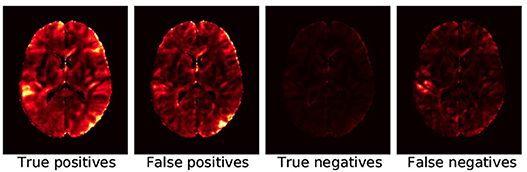
\includegraphics[scale=0.4]{assets/images/lrp_alzheimer.png}
    \caption{
        \textbf{Priemerná relevancia (z metódy LRP - $\beta = 0$) pozorovaní podľa spôsobu zaradenia výslednej predikcie} Najviac relevancie je na miestach so žltou farbou. \cite{bohle2019layer}
    }
    \label{fig:lrp_alzheimer}
\end{figure}

\section{Spracovanie obrazu \label{cap:image_processing}}

Keďže pri diagnostike Alzheimerovej choroby sa pracuje s rádiologickými snímkami, čo sú trojrozmerné obrazové dáta, pri jej detekcii neurónovými sieťami je potrebné tieto dáta spracovať technikami spracovania obrazu.

Metódy spracovania obrazu podľa \citeauthor*{chen2004electrical} \cite{chen2004electrical} rozdeľujeme do nasledovných kategórií:
\begin{itemize}
    \item vylepšovanie obrazu (angl. image enhancement)
    \item rekonštrukcia obrazu (angl. image restoration)
    \item analýza obrazu (angl. image analysis)
    \item kompresia obrazu (angl. image compression)
\end{itemize}

Pri \textbf{vylepšovaní obrazu} je obraz upravovaný predovšetkým heuristickými technikami \cite{chen2004electrical}, môže sa napríkald jednať o upravenie jasu, kontrastu alebo farieb. Cieľom \textbf{rekonštrukcie obrazu} je zrekonštruovať poškodené časti obrazu, napr. pri fotografiách to môžu byť ich vyblednuté časti. Metódy \textbf{analýzy obrazu} umožňujú obraz spracovať tak, že je možné z neho automaticky získať (extrahovať) informácie \cite{chen2004electrical}. Príkladmi analýzy obrazu je segmentácia obrazu, extrakcia hrán alebo analýza textúry. \textbf{Kompresia obrazu} umožňuje zmenšenie veľkosti obrazu znižovaním počtom potrebných bitov na jeho reprezentáciu \cite{chen2004electrical}. Môže sa jednať o zmenšenie rozmerov obrazu, alebo počtu farieb potrebných na jeho reprezentáciu.

V našej doméne budeme pracovať so všetkými týmito technikami. Ako príklad môžem uviesť odstránenie takých častí obrazu, ktoré nepredstavujú mozgové tkanivo (BET - \citeauthor*{smith2002fast} \citeyear{smith2002fast}). Táto technika je kombináciou analýzy obrazu - identifikácia častí na odstránenie a vylepšenia obrazu - samotné odstránenie tých častí. Kompresia obrazu sa používa, v časti predspracovania pred tým ako je samotný snímok použitý ako vstup do neurónovej siete. Metódy rekonštrukcie obrazu sa bežne v tejto oblasti nepoužívajú, avšak my by sme ich chceli v našej práci použiť pri vytváraní novej metódy, preto sa im budeme bližšie venovať.

\subsection{Rekonštrukcia obrazu}

Metódy rekonštrukcie obrazu, alebo inak nazývané aj dokreslenia obrazu (angl. inpainting), podľa \citeauthor{6544390} \cite{6544390} môžeme zaraďiť do nasledovných kategórií:
\begin{itemize}
    \item dokresľovanie založené na syntéze textúr
    \item poloautomatické a rýchle digitálne dokresľovanie
    \item dokresľovanie založené na parciálnej diferenciálnej rovnici
    \item dokresľovanie na základe predlohy a vyhľadávania
    \item hybridné dokresľovanie
\end{itemize}

Tieto metódy sa líšia rýchlosťou dokresľovania, schopnosti dokreslovať veľké/malé plochy a predovšetkým kvalitou dokreslenia. Metódy dokresľovania založené na syntéze textúr fungujú dobre pre väčšie chýbajúce oblasti, avšak v ich výsledku môžu vzniknúť nežiadúce hrany \cite{6544390}. Dokresľovanie na základe predlohy má zas problémy so zakrivenými štruktúrami \cite{6544390}. Obr. \ref{fig:inpainting} zobrazuje príklady použitia niektorých techník dokreslenia obrazu.

\begin{figure}[h!]
    \centering
    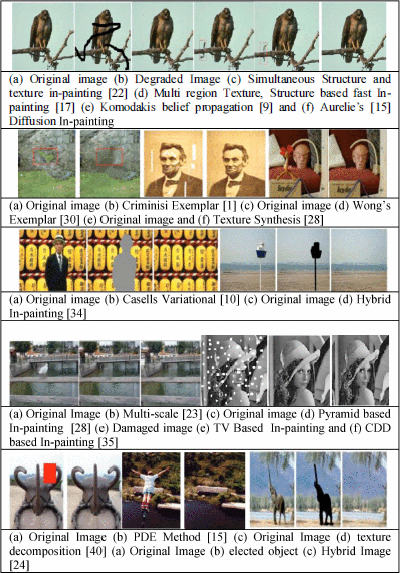
\includegraphics[width=11.25cm]{assets/images/inpainting.png}
    \caption{
        \textbf{Príklady dokreslenia obrázkov rôznymi metódami \cite{6544390}.}
    }
    \label{fig:inpainting}
\end{figure}


% LOL - Toto neviem ci hej
% LRP sa taktiež ukázala ako pomerne robustná metóda pre overovanie správnosti modelu, pretože oproti iným metódam na interpretovanie neurónových sietí produkuje stabilnejšie výsledky pri opakovanom trénovaní modelu (tepelné mapy z LRP sú porovnávané po každej epoche s tou predchádzajúcou) \cite{esmaeilzadeh2018end}.

% \section{Výskumné tézy}

% \paragraph{Kombináciou existujúcich metód na interpretovanie a vysvetľovanie rozhodnutí neurónových sietí je možné zlepšiť interpretovateľnost / vysvetliteľnosť nerónovej siete predikujúcej Alzheimerovu chorobu.} Existujúce práce sa predovšetkým zaoberali porovnávaním jednotlivých metód interpretácia/vysvetľovania predikcie.

% \paragraph{Uplatnením interpretovateľnosti a vysvetliteľnosti neurónových sietí je možné vytvoriť podporný systém pre doktorov na diagnostiku Alzheimerovej choroby.} \citeauthor{bohle2019layer} uvádzajú LRP ako metódu na vysvetľovanie invididuálnych rozhodnutí neurónovej siete natrénovanej na diagnostiku Alzheimerovej choroby. Využitím (nielen) tejto metódy môžeme skúsiť vytvoriť podporný systém pre doktorov.

% \paragraph{Syntézou rôznych typov snímok je možné dosiahnuť presnejšie výsledky pri diagnóze Alzheimerovej choroby pomocou neurónových sietí.} Súčasné state-of-the-art riešenie \cite{esmaeilzadeh2018end} na dátovej množine ADNI využíva predovšetkým snímky z MRI, táto dátová množina avšak obsahuje aj snímky z PET. Využitím oboch typov snímkov môžeme skúsiť zlepšiť úspešnosť tohto modelu.

% % Mozne vyuzit LRP pri trenovani modelu

% \paragraph{Metóda LRP je využiteľná pri vysvetľovaní rozhodnutí neurónovej siete predikujúcej Alzheimerovuj chorobu zo snímkov pacientov s miernym kognitývnym poškodením (angl. mild-cognitive impairment).} \citeauthor{bohle2019layer} overovali metódu LRP na snímkoch pacientov s Alzheimerovou chorobou a zdravých jedincoch, túto metódu avšak neoverovali na pacientoch s miernym kognitývnym poškodením, čo diskutujú v závere ako možnú oblasť výskumu pre ďalšie štúdie.

% \paragraph{Metódy interpretovateľnosti neurónových sietí je možné využiť na určenie správnosti natrénovaného modelu (neurónovej siete natrénovanej na diagnostiku Alzheimerovej choroby).} \citeauthor{bohle2019layer} označili vedenú spätnú propagáciu ako metódu na zistenie oblastí snímku mozgu, na ktoré je neurónová sieť senzitívna. Porovnaním výstupu tejto metódy s mapou mozgu môžeme skúsiť určiť správnosť neurónovej siete, tj. či sa neurónová sieť rozhoduje na základe tých častí mozgu, ktoré sa v medicíne používajú na diagnostiku Alzheimerovej choroby.

\section{Zhrnutie}

Alzhemierova choroba je bez pochyby veľmi nebezpečnou chorobou, keďže nie je ''iba'' o strate pamäti ale patrí k častým príčinám smrti (Sek. \ref{sec:ad}). Diagnostika tejto choroby pozostáva najmä z neuropsychometrických testov a analýzy rádiologických snímkov (napr. z PET, MRI). V súčasnosti tieto rádiologické snímky posudzujú doktori samotný. Práve tu je priestor pre umelú inteligenciu, aby im pri posudzovaní týchto snímkov pomohla.

V doméne obrazových dát sa používajú najmä konvolučné neurónové siete, pretože majú veľmi dobrú schopnosť naučiť sa rozoznávať špecifické objekty z obrázka. Konvolučné neurónové siete sa v nižších vrstvách naučia rozoznávať jednoduchšie tvary/hrany a vo vyšších zložitejšie šruktúry až celé objekty. Keďže jednou z možností diagnostiky Alzheimerovej choroby je diagnstika pomocou rádiologických snímkov, je možné použiť neurónové siete práve pri detekcii tohto ochorenia.

Neurónovým sieťam sa doteraz podarilo dosiahnuť veľmi dobré výsledky pri detekcii Alzhemerovej choroby, niektoré state-of-the-art riešenia dosahujú presnosť až \textbf{95.09\%} (\citeauthor*{suk2016deep} \citeyear{suk2016deep}). S takto vysokou úspešnosťou môžu byť veľmi dobrým pomocníkom doktorov. Do úvahy však musíme zobrať, že tieto výsledky boli dosiahnuté bez klasifikácie MCI pacientov. V reálnom svete doktora navštívia všetky typy pacientov - CN, MCI a AD. V tomto prípade neurónové siete dosahujú rádovo nižšiu presnosť (\textbf{61.1\%}, \citeauthor*{bohle2019layer} \citeyear{bohle2019layer}). Niektoré práce dosiahli tieto výsledky použitím informácií o veku a pohlaví pacienta. Keďže pravdepodobnosťou výskytu Alzheimerovej choroby po dovŕšení 85 rokov života je až 50\% (Sek. \ref{sec:ad}), je možné, že sa pri vyššom veku pacienta model začne rozhodovať najmä na základe tejto informácie a nie na základe obrazových dát. Zároveň to však môže neurónovej sieti pomôcť, ak nebude brať tento atribút ako hlavný indikátor Alzheimerovej choroby, ale skôr ako pomocný atribút, ktorý bude meniť jej správanie u rôznych typov pacientov. Tu je však dôležité, takúto neurónovú sieť podrobiť dôkladnou analýzou jej rozhodnutí. Osobne si ale myslím, že v produkčnom modeli by sa tento atribút mal vynechať. 

Ďaľším problémom neurónových sietí je, že sa správajú ako čierne skrinky. Preto je potrebné ich rozhodnutia interpretovať, aby bolo pre doktora zrejmé na základe čoho neurónová sieť urobila svoju predikciu. V tomto práve môžu pomôcť metódy na vysvetľovanie rozhodnutí neurónovej siete (tzv. white-box metódy), alebo iné black-box metódy vysvetľovania rozhodnutí modelov (napr. RISE, LIME...).

Bežnému používaniu neurónových sietí ako pomocníka pre doktorov, nebráni len ich vysvetliteľnosť, ale aj ich schopnosť detekcie ochorenia, keďže aj tu je priestor na zlepšenie - napr. úspešnosti klasifikácie do CN, MCI a AD.

Pre pochopenie správania sa neurónových sietí poznáme metódy jej interpretovania a vysvetľovania jej rozhodnutí. Interpretovaním neurónovej siete zisťujeme, ako vyzerá vzorové pozorovanie pre jednu z tried, ktorú klasifikuje. Vysvetľovaním jej rozhodnutí zas zisťujeme na základe čoho neurónová sieť spravila svoje rozhodnutie, a teda ktoré zo vstupných vlastnosti pozorovania ju navideli k zaradeniu do určitej triedy. Niektoré z týchto metód (LRP a vedená spätná propagácia) už boli použité pri vysveľovaní rozhodnutí neurónových sietí detekujúcich Alzheimerovu chorobu, avšak zatiaľ len pri binárnej klasifikácii pacientov.

% TODO
% 1-3 strany
% Vlastnymi slovami zhrnut state of the art
% Aky je stav, ake su trendy
% Co ste si z analyzy zobrali pre svoju pracu -> vychodiska
    
    % Goals
    % \clearpage\null
    \chapter{Ciele práce \label{sec:goals}}

Vychádzajúc zo zadania projektu a na základe poznatkov nadobudnutých z analýzy domény a problému, sme si stanovili nasledovné ciele.

\section{Vytvorenie novej, alebo vylepšenie existujúcej metódy pre vysvetľovanie rozhodnutí neurónových sietí \label{sec:goals_1}} 

Existujú rôzne metódy pre vysvetľovanie rozhodnutí neurónových sietí. Niektoré z nich potrebujú poznať model, ako napríklad LRP (ktorá pracuje iba s neurónovými sieťami), iné nepotrebujú, a je ich teda možné použiť na ľubovoľný typ modelu. Každá z metód má iné výhody/nevýhody preto je tu priestore na vytvorenie alebo vylepšenie existujúcej metódy. V prípade vylepšenia existujúcej metódy je nutné túto metódu porovnať najmä s vylepšovanou metódou a následne s inými metódami. Cieľom je teda vytvoriť novú metódu, ktorá vytvára presnejšie vysvetlenia ako iné metódy, alebo vylepšiť existujúcu metódu, ktorá vytvára presnejšie vysvetlenia ako metóda, z ktorej vychádza. Zároveň táto metóda ma byť použiteľná na medicínske obrazové dáta.

\section{Využitie vytvorenej metódy na určenie miery správnosti modelu neurónovej siete detegujúcej Alzheimerovu chorobu \label{sec:goals_2}}

Pri neurónových sieťach detekujúcich Alzheimerovu chorobu je dôležité, aby sa naučili klasifikovať pacientov na základe relevatných čŕt z rádiologických snímkov. Práve preto je potrebné určiť mieru správnosti modelu podľa toho či sa model rozhoduje práve na základe týchto čŕt a nie iných. Na to sa využívajú metódy na vysvetľovanie rozhodnutí neurónových sietí, v tomto prípade sa použije novovytvorená metóda. Cieľom je teda určiť správnosť modelu detegujúceho Alzheimerovu chorobu pomocou vytvorenej metódy pre vysvetľovanie rozhodnutí neurónovej siete.

    
    % Design
    % \clearpage\null
    \chapter{Návrh riešenia}

Pre použitie neurónových sietí v bežnej praxi doktorov pri diagnostike Alzheimerovej choroby je nevyhnutné, aby sa rozhodnutia neurónových sietí dali vysvetliť. Preto navrhujeme metódu na vyvsvetľovanie rozhodnutí neurónových sietí, ktorú overíme na MRI snímkoch u pacientov (CN, MCI a AD).

Vychádzajúc cieľa práce \textit{\ref{sec:goals_1} Vytvorenie novej alebo vylepšenie existujúcej metódy pre vysvetľovanie rozhodnutí neurónových sietí} navrhujeme metódu, ktorá vychádza z už existujúcej metódy \textit{RISE} (Sek. \ref{sec:rise}). Táto metóda dosiahla veľmi dobré výsledky oproti metódam GradCAM a LIME a považujem ju teda vhodný základ pre ďaľšie vylepšenia. Metóda RISE funguje na princípe zakrývania častí obrázka (tak ako iné perturbačné/oklúzne metódy) jednou hodnotou (tj. farbou). Po takomto prekrytí avšak nevznikajú žiadné ostré hrany, ktoré by mohli neurónovú sieť mýliť ako u iných metódach, ktoré fungujú na princípe zakrývania častí obrazu. Keďže metóda RISE bola pôvodne použitá na obrázky vo farebnom priestore RGB, tento prekryv sa zvyčajne robí v čiernej farbe - tj. v (r = 0, g = 0, b = 0). MRI snímky nepoužívajú žiadnu farebnú schému, ale zachytávajú intenzitu (hodnoty sú zväčša reálne čísla). V tomto prípade môžeme zakrývať maximálnou alebo minimálnou hodnotou (minimálna hodnota je ekvivalentná RGB v prípade šedej). Toto zakrytie môže byť práve ďalším zdrojom zmätenia pre neurónovú sieť, keďže úbytky tkaniva sú vyjadrené nízkymi hodnotami na snímkoch. Preto navrhujeme zakrývané miesta dokresliť určitou metódou spracovania obrazu (Sek. \ref{cap:image_processing}) alebo na zakrytie použiť inú hodnotu.
Pôvodná metóda bola ale narvhnutá pre obrázky (tj. 2D) a nie 3D volumetrické dáta, preto budeme musieť metódu RISEI upraviť aby vedela pracovať s 3D dátami - tj. budeme generovať 3D masky a podobne.

\section{RISEI - Randomized Input Sampling for Explanation with Inpainting \label{sec:risei}}

Metódu sme pomenovali \textit{Randomized Input Sampling for Explanation with Inpainting} (tj. náhodné vzorkovanie vstupu pre vysvetlovanie s dokreslovaním) so skratkou \text{RISEI}.

Keďže metóda vychádza už z existujúcej metódy, časť našej metódy je samozrejme rovnaká. Proces vytvorenia vysvetlenia klasifikácie (Obr. \ref{fig:risei_heatmap_generation}) do triedy $T$ pre obrázok $O$ modelom je teda nasledovný:

\begin{enumerate}
    \item Vytvorenie \textit{N} náhodne zamaskovaných obrázkov z obrázka $O$.
    \item Vloženie zamaskovaných obrázkov do modelu a následné získanie pravdepodobností pre triedu $T$.
    \item Vytvorenie a vizualizácia vysvetlenia pomocou tepelnej mapy.
\end{enumerate}

\begin{figure}[h!]
    \centering
    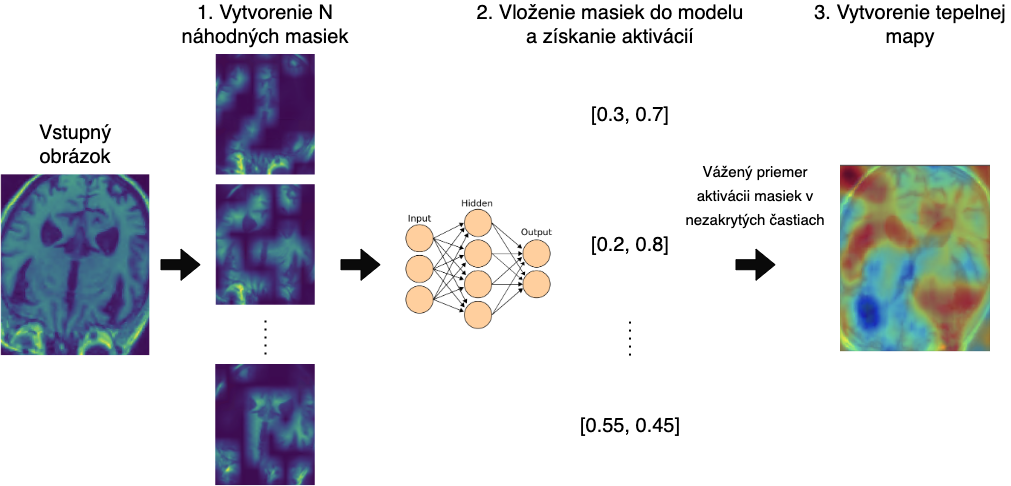
\includegraphics[scale=0.35]{assets/images/risei_heatmap_generation.png}
    \caption{Proces vysvetlenia klasifikácie - vytvorenia tepelnej mapy.}
    \label{fig:risei_heatmap_generation}
\end{figure}

Toto sú 3 hlavné kroky z ktorých pozostáva táto metóda, ďalej bližšie popíšeme jednotlivé z nich.

\paragraph{Vytvorenie náhodne zamaskovaných obrázkov.}

Vytvorenie náhodne zamaskovaných obrázkov tiež pozostáva z niekoľkých krokov, pričom niektoré z nich môžu byť vykonávané paralelne. Tento krok sme znázornili diagramom (Obr. \ref{fig:risei_diagram}). Masky sa vytvárajú paralelne, pretože ''čierna'' maska ma jemné hrany a na dokreslenie potrebujeme naopak masku s ostrými hranami.

\begin{figure}[h!]
    \centering
    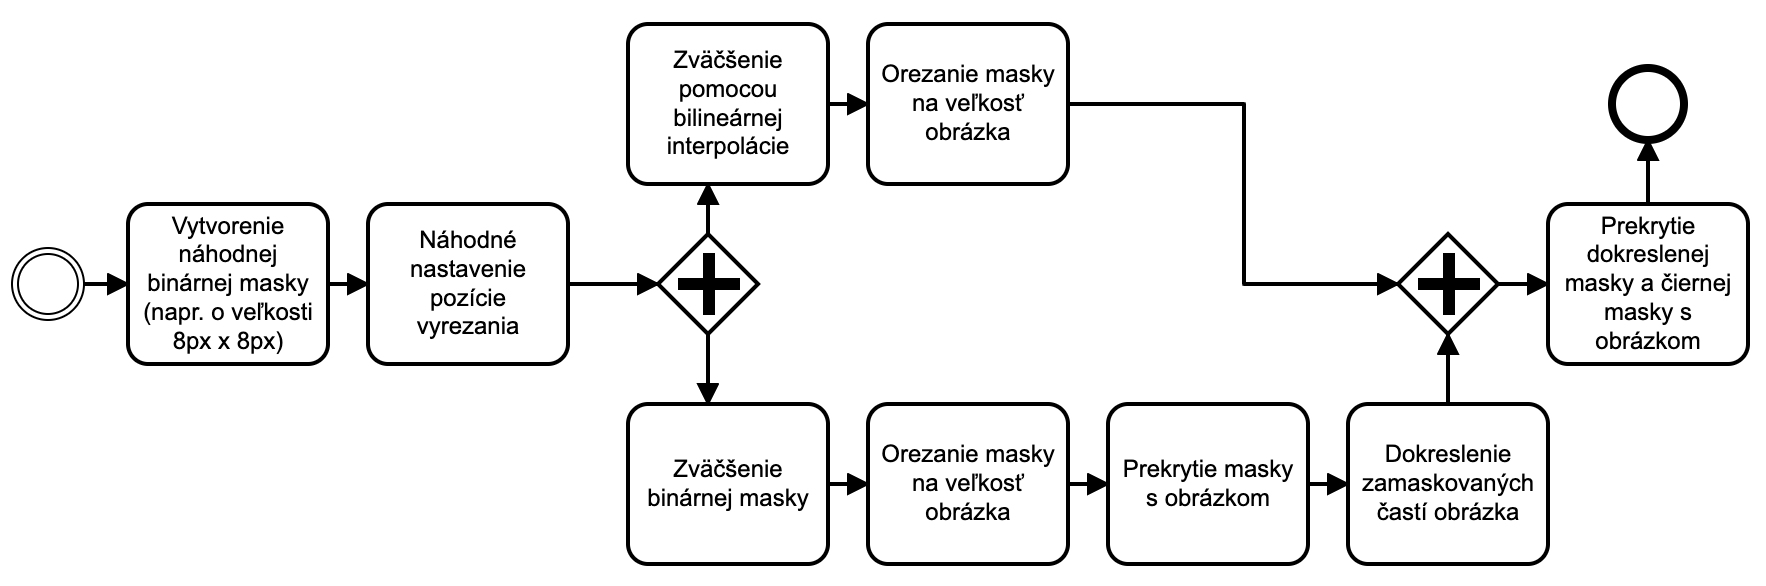
\includegraphics[scale=0.45]{assets/images/risei_diagram.png}
    \caption{BPMN diagram generovania jedného obrázka prekrytého maskou}
    \label{fig:risei_diagram}
\end{figure}

Oproti metóde \textit{RISE} vytvárame o jednu masku naviac, a teda je originálny obrázok prekrytý s viacerými maskami. Jednotlivé masky cez seba prekryjeme, pričom každej z nich nastavíme určité množstvo priehľadnosti. S týmto pomerom môžeme ďalej experimentovať a výsledky porovnávať. Môžeme porovnať použitie iba dokreslenej masky s iba ''čiernou'' maskou a tiež s použitím oboch v rôznych pomeroch.

Vytvorenie ''čiernej'' masky je rovnaké, ako pri metóde \textit{RISE}. Dokreslená maska vznikne dokreslením zakrytých (zamaskovaných) častí obrázka pomocou jedného z algoritmov na dokreslovanie (angl. inpainting). Tieto algoritmy sme popísali v sekcii \ref{cap:image_processing} Spracovanie obrazu. Obrázok \ref{fig:risei_inpainting_example} je príkladom dokreslenia častí vzorového obrázka na základe masky náhodne vygenerovanej masky (tento príklad je v 2D, naša metóda bude pracovať s 3D). V našej metóde budeme experimentovať s rôznymi hodnotami prekrytia (priemer, maximum, minimum, medián).

\begin{figure}[h!]
    \centering
    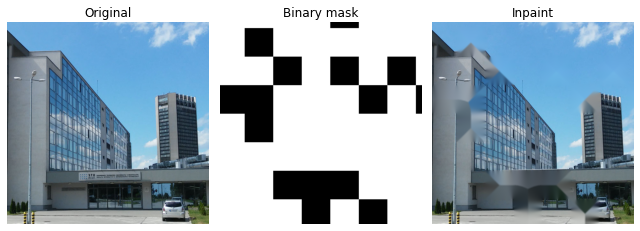
\includegraphics[width=13cm]{assets/images/risei_inpainting_example.png}
    \caption{Niektoré časti vzorového obrázoka (vľavo) boli dokreslené podľa náhodne vygenerovanej binárnej masky (v strede). Výsledný obrázok (vpravo) môže byť ešte prekrytý ''čiernou'' maskou s určitou priehľadnosťou.}
    \label{fig:risei_inpainting_example}
\end{figure}

\paragraph{Vytvorenie a vizualizácia vysvetlenia pomocou tepelnej mapy.}

Tento krok je identický s originálnou metódou \textit{RISE}. Nasledovný vzorec \ref{eq:risei_heatmap_1} vyjadruje výpočet dôležitosti $I$ pre každý voxel $[x, y, z]$ snímky, kde $n$ je počet všetkých zamaskovaných snímok. Funkcia $p(k, x, y, z)$ vracia vracia predikciu (tj. aktiváciu v kontexte neurónových sietí) pre predikovanú triedu (v prípade binárnej klasifikácie) z modelu pre zamaskovaný snímok $k$. Funkcia $c(k, x, y, z)$ vracia mieru zakrytia/dokreslenia maskou, pričom $H(c) = <0, 1>$, kde $1$ znamená úplné prekrytie/dokreslenie a $0$ žiadne prekrytie/dokreslenie. Rovnako, ako metóde \textit{RISE}, počítame vážený priemer.

\begin{equation} 
    I_{x, y, z} = \frac{\sum_{k}^{n} p(k, x, y, z) * (1 - c(k, x, y, z))}{\sum_{k}^{n} p(k, x, y, z)}
    \label{eq:risei_heatmap_1}
\end{equation}

Navrhovaná metóda do orignálnej metódy pridáva niekoľko parametrov a najmä výpočtovo náročné dokreslovanie, preto bude nutné nájsť vhodné nastavenie parametrov, aby výpočet vysvetlenia nebol príliš časovo náročný. Práve výpočtová náročnosť môže byť jednou zo slabín tejto metódy. Takisto aj samotná dokreslená časť obrázka môže byť príčinou zmätenia neurónovej siete.

\section{Overenie riešenia \label{sec:evaluation_design}}

Našu metódu budeme najskôr porovnávať s originálnou metódou RISE (tj. či sa nám podarilo vytvoriť lepšiu metódu) a následne s inou existujúcou metódou (LRP, GradCAM, Guided Backprop alebo Guided GradCAM). Z týchto metód je najviac vhodná metóda LRP, keďže už bolo jej použitie pri vysvetľovaní rozhodnutí neurónových sietí detekujúcich Alzheimerovu chorobu (Sekcia \ref{sec:ad_nn_explanation}) skúmané. Tieto experimenty môžeme vykonávať na CN a AD vzorkách; a aj na CN, MCI a AD vzorkách. Budeme sledovať kvalitu navrhnutej metódy (oproti ostatným metódam) a na základe týchto tepelných máp budeme vyhodnocovať mieru správnosti modelu.

\subsection{Dátová sada} Experimenty budeme vykonávať na dátovej sade ADNI, ktorá obsahuje MRI snímky AD pacientov. Táto dátová sada bola použitá aj na trénovanie state-of-the-art modelu na diagnsotiku Alzheimerovej choroby \cite{esmaeilzadeh2018end}, ale aj pri vysvetľovaní rozhodnutí neurónovej siete pomocou LRP \cite{bohle2019layer}. Na tejto dátovej sade budeme musieť vykonať rovnaké predspracovanie ako \citeauthor*{bohle2019layer}, aby sme sa s ich výsledkami mohli porovnať. Prípadne môžeme vykonať vlastné predspracovanie, ale budeme musieť vykonať aj experimenty s metódou LRP.

\subsection{Experimenty \label{sec:design_experiments}}

Najskôr budeme vyhodnocovať nami navrhnutú metódu pomocou sledovania kvality tepelných máp. Následne budeme overovať správnosť modelu pomocou nami navrhnutej metódy, avšak je nutné aby metóda generovala kavlitné tepelné mapy.

\subsubsection{Určenie kvality metódy vysvetľovania rozhodnutí modelu \label{sec:evaluation_design_method_quality}}

Kvalitu metódy vysvetľovania rozhodnutí modelu budeme sledovať určovaním kvality tepelnej mapy. Tá v kontexte našej práce hovorí o tom, do akej miery táto mapa odzrkadľuje to, na základe čoho sa model rozhoduje. Toto budeme merať metrikami \textit{insertion (AUC)} a \textit{deletion (AUC)}, ktoré sme bližšie popísali v sekcii \ref{sec:rise}. Táto metrika nám povie, aká dobrá je naša metóda na vysvetľovanie.

Keďže naša metóda generuje tepelné mapy pomocou vygenerovania veľkého množstva náhodných masiek, je vhodné skúmať, ako sú tieto tepelné mapy konzistentné pri niekoľkých požitiach metódy na tom istom MRI snímku. Konzistentnosť máp môžeme merať pomocou podobnosti medzi jednotlivými tepelnými mapami vygenerovaními pre tú istú snímku (napr. ako súčet absolútných hodnôt rozdielov medzi voxelmi v oboch tepelných mapách). čím je táto podobnosť väčšia, tým je metóda pri generovaní máp viac konzistentná.

\subsubsection{Určenie správnosti modelu \label{sec:heat_maps_and_model_segmentation_masks}}

Správnosť modelu budeme určovať na na základe tepelných máp vytvorených pomocou metódy na vysvetľovanie predikcií modelu. Budeme overovať do akej miery dávajú tepelné mapy zmysel v kontexte skutočnej anatómie mozgu, tj. či tepelná mapa pre správnu predikciu ukazuje na klinicky relevantné oblasti mozgu. Sledujeme, že či tepelná mapa nehovorí o tom, že sa model rozhodol na základe takej oblasti mozgu, z ktorej sa Alzheimerova choroba nedá zistiť. Veľkú úlohu pri určovaní správnosti modelu zohráva aj kvalita natrénovaného modelu, tú môžeme merať pomocou metrík z práce od \citeauthor*{bohle2019layer} v ktorej sa autori zaoberali vyhodnocovaním tepelných máp vypočítaných pomocou metódy LRP. Tieto metriky sú nasledovné (relevancia je v našom prípade teplota na tepelnej mape):

\begin{itemize}
    \item súčet relevancie v jednotlivých častiach mozgu (podľa segmentačných masiek) pre AD a CN
    \item hustota relevancie v jednotlivých častiach mozgu (podľa segmentačných masiek) pre AD a CN, berie ohľad na veľkosť danej časti mozgu
    \item prírastok relevancie v jednotlivích častiach mozgu (podľa segmentačných masiek) vypočítaný ako pomer priemernej relevancie každej triedy v danej časti mozgu
\end{itemize}

\section{Zhrnutie}

V tejto kapitole sme navrhli metódu na vysvetľovanie rozhodnutí modelov strojového učenia a spôsob jej implementácie. Navrhnutú metódu budeme overovať na neurónových sieťach detegujúcich Alzheimerovu chorobu s cieľom odhaľovania nesprávnych rozhodnutí.

    
    % Implementation
    \clearpage\null
    \chapter{Implementácia}

\section{Metóda RISEI}

Metódu RISEI sme sa rozhodli implementovať v jazyku Python, keďže plánujeme používať knižnice pre strojové učenie akými sú \textit{tensorflow} či \textit{scikit-learn}.

\subsection{Generovanie masiek}

Na základe BPMN diagramu (Obr. \ref{fig:risei_diagram}) sme implementovali proces generovania masiek. Generovanie masiek prebieha paralelne vo viacerích procesoch použitím knižnice Python \textit{multiprocessing}. Metóda RISE pracuje s trojrozmernými dátami, avšak diagramy v tejto sekcii zobrazujú snímky a masky v 2D (konkrétne určitú vrstvu z 3D snímku) kvôli jednoduchšej vizualizácii. V tejto sekcii popíšeme jednotlivé kroky generovania masiek.

\paragraph{Vytvorenie náhodnej binárnej masky}

Náhodné binárne masky generujeme pomocou knižnice \textit{numpy}. Pomocou nasledovného kódu vygenerujeme $N$ náhodných masiek 3D binárnych matice. Obr. \label{fig:risei_inpainting_example} zobrazuje takúto binárnu maticu, ale v 2D. \textit{size} (veľkosť) a \textit{probability} (pravdepodobnosť) sú hyper-parametrami RISEI metódy. \textit{size} hovorí o veľkosti generovanej masky, čím je toto číslo väčšie tým bude výsledná maska viac fragmentovaná na malé plochy. \textit{probability} hovorí o tom, s akou pravdepodobnosťou daná plocha neprekrytá maskou. RISE používa predvolenú hodnotu \textit{size = 8}.

\begin{lstlisting}
    binary_masks = np.random.rand(N, size, size, size) < probability
\end{lstlisting}

\begin{figure}[h!]
    \centering
    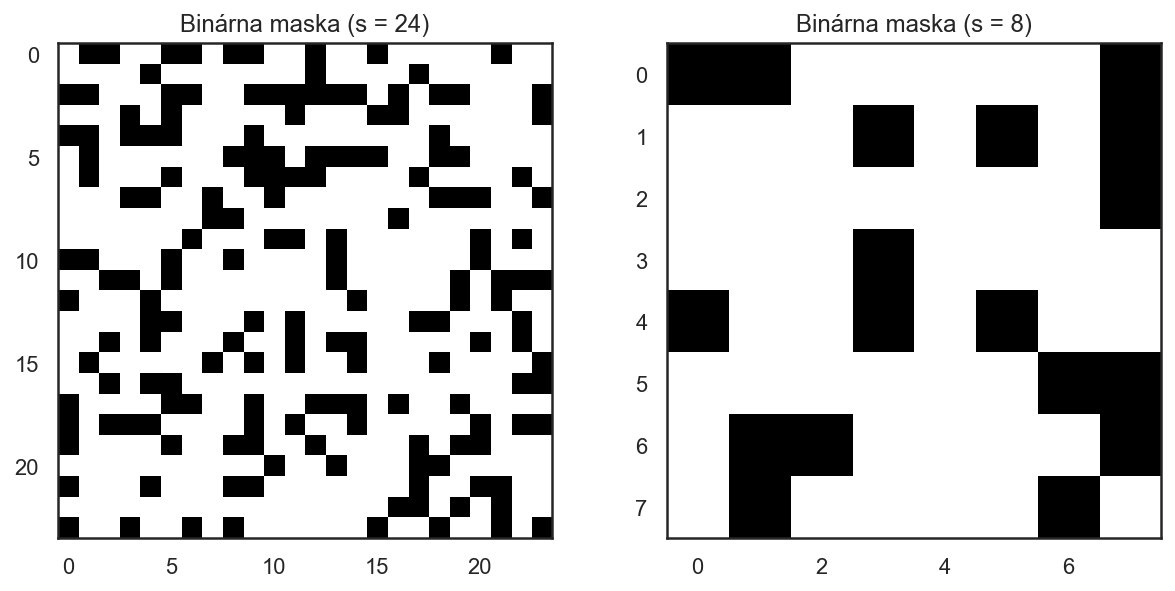
\includegraphics[width=13cm]{assets/images/binary_mask.png}
    \caption{Porovnanie dvoch binárnych masiek s rôznou veľkosťou (\textit{size}), čím väčšia veľkosť, tým je obrázok viac fragmentovaný.}
    \label{fig:binary_mask}
\end{figure}

\paragraph{Náhodné nastavenie pozície vyrezania, zväčšenie binárnej masky a orezenie na veľkosť obrázka}

Binárnu masku zväčšíme na veľkosť vstupného snímku plus menší offset (o veľkosti size). Následne zo zväčšenej masky na náhodnej pozícii vyrežeme masku o veľkosti vstupného snímku (Obr. \ref{fig:binary_mask_resized}). Táto maska určuje, ktoré miesta na snímku bude treba dokresliť - biele miesta, čiže jednotky. Tento krok v pôvodnej implementácii RISE nie je.

\begin{figure}[h!]
    \centering
    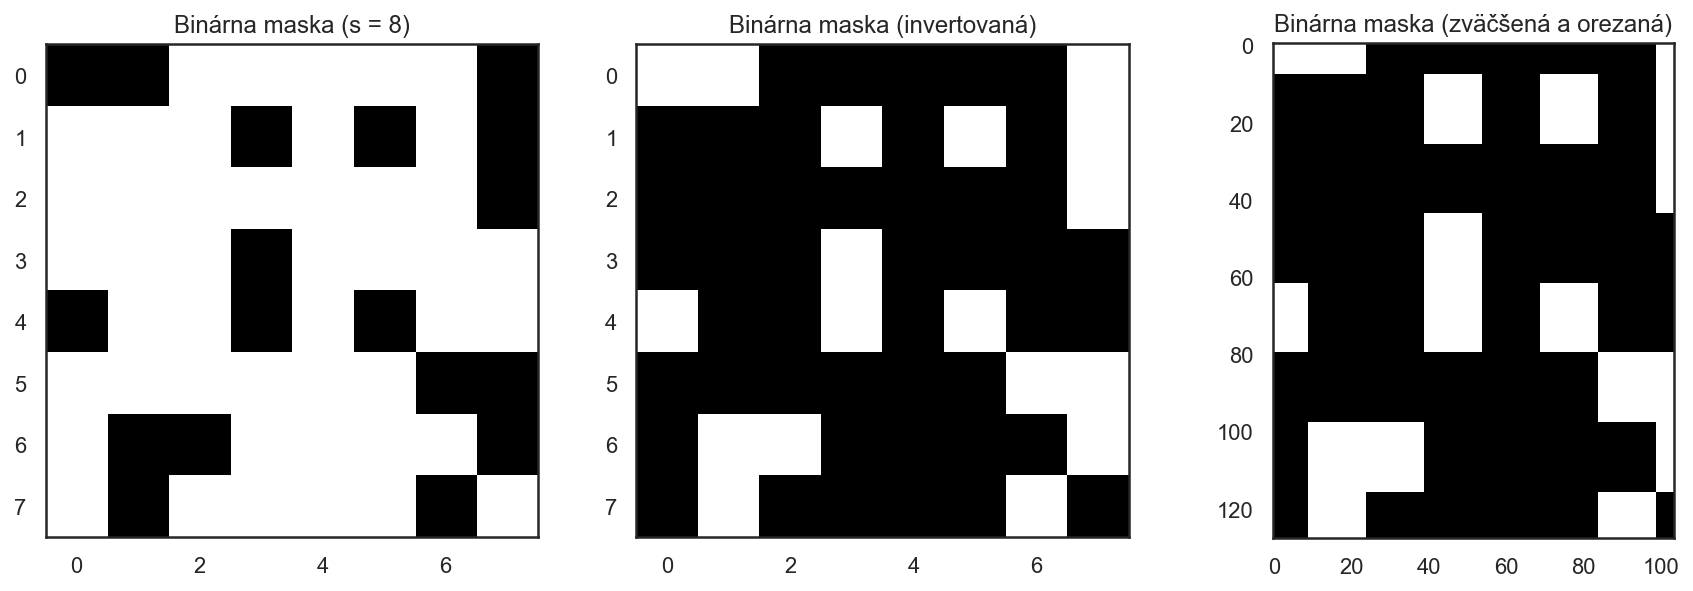
\includegraphics[width=13cm]{assets/images/binary_mask_resized.png}
    \caption{Vygenerovaná maska je zväčšená a orezaná na veľkosť vstupného snímku (ten je o veľkosti $[104, 128, 104]$ pričim na obrázkoch je vizualizovaná druhá a tretia dimenzia). Úplne vľavo je binárna maska o veľkosti $8$. V strede je invertovaná binárna maska (kvôli ďaľšiemu pracovanou s ňou) a vpravo je orezaná binárna maska o veľkosti vstupného snímku.}
    \label{fig:binary_mask_resized}
\end{figure}

\paragraph{Zväčšenie pomocou bilineárnej interpolácie a orezanie masky na veľkosť obrázka}

Tak ako v poôvodnej implementácii RISE, vytvoríme ''čiernu'' masku na zakrytie častí obrázku. Pôvodnú binárnu masku pomocou bilineárnej interpolácie (funkcia \textit{resize} z knižnice \textit{scikit-learn}) zväčšíme na veľkost vstupného snímku plus menší offset, následne vyrežeme na náhodnej pozicii masku o veľkosti vstupného snímku (táto náhodná pozícia je rovnaká ako pri orezávani binárnej masky bez interpolácie, preto je v BPMN diagrame v samostatnom kroku).

\begin{figure}[h!]
    \centering
    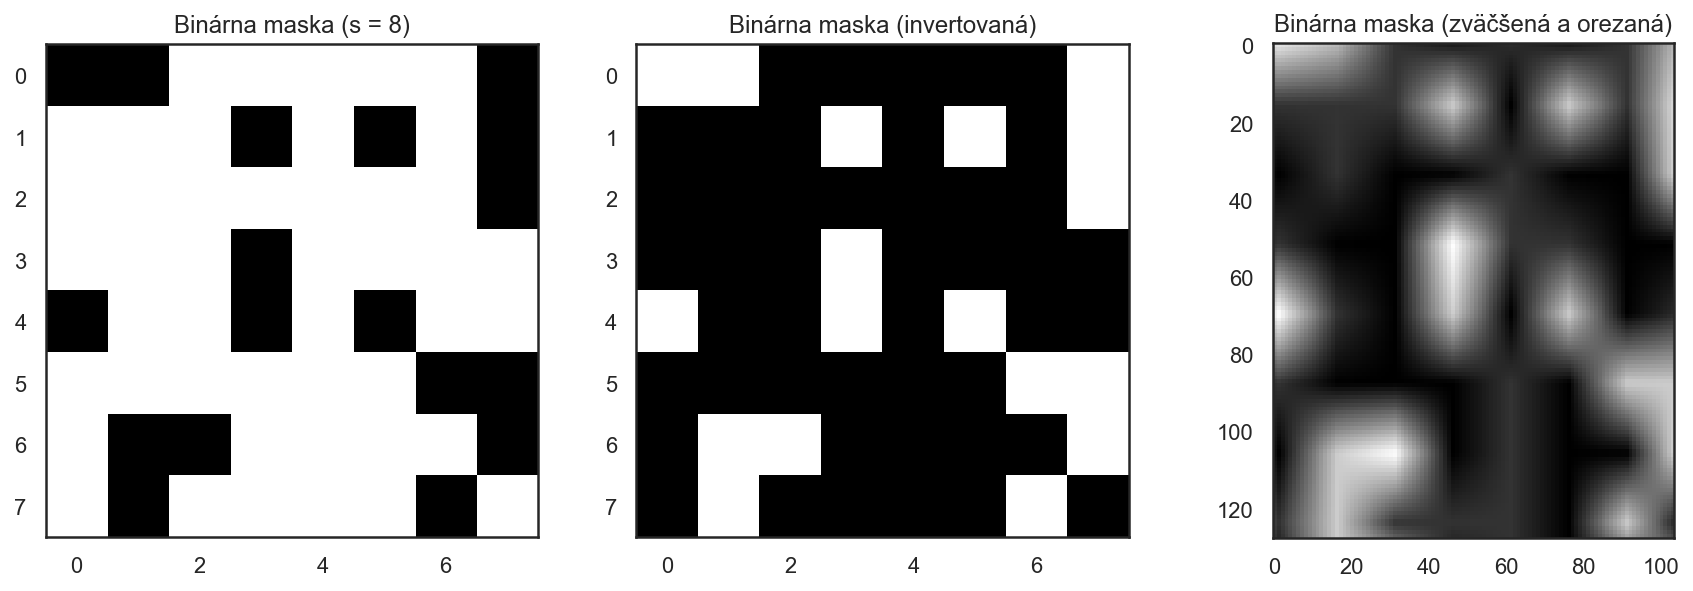
\includegraphics[width=13cm]{assets/images/interpolated_mask.png}
    \caption{Vygenerovaná maska je zväčšená pomocou bilineárnej interpolácie a orezaná na veľkosť vstupného snímku (ten je o veľkosti $[104, 128, 104]$ pričim na obrázkoch je vizualizovaná druhá a tretia dimenzia). Úplne vľavo je binárna maska o veľkosti $8$. V strede je invertovaná binárna maska (kvôli ďaľšiemu pracovanou s ňou) a vpravo je orezaná interpolovaná ''čierna'' maska o veľkosti vstupného snímku.}
    \label{fig:interpolated_mask}
\end{figure}

\paragraph{Prekrytie masky s obrázkom a dokreslenie zamaskovaných častí obrázka}

Keďže pracujeme nad trojrozmernými dátami, pokúsili sme sa použiť dokreslovanie obrázka v 3D. Na to sme sa pokúsili použiť funkciu \textit{inpaint} s knižnice \textit{scikit-image}, avšak dokreslenie jednej masky bolo veľmi časovo náročné (trvanie bolo až v minútach kde dokreslenie v 2D je v sekundách) a my ich potrebujeme generovať tisíce, preto sme trojrozmerného dokreslovania upustili.

Dokreslovanie dvojrozmerných snímkov z 3D snímku má avšak svoje nevýhody. Nech máme snímky o veľkosti $[z, y, x]$, pri 2D dokreslení musíme dokreslovať $z$ snímkov o veľkosti $[y, x]$ (alebo $y$ snímkov o veľkosti $[y, x]$, alebo $x$ snímkov o veľkosti $[y, z]$). Pri takomto dokreslovaní, dokreslenie z pohľadu $[y, x]$ vyzerajá byť správne, avšak z iného pohľadu, napr. $[z, x]$ sa javí byť dokreslenie nesprávne, najmä kvôli vzniknutým ostrím hranám (Obr. \ref{fig:inpaint_3x_2d}). Toto sme sa pokúsili obýsť tak, že dokreslujeme zo všetkých troch pohľadov a robíme priemer pre každý voxel zo všetkých troch dokreslení. Takto je výsledok o niečo lepší, tj. z každej strany je dokreslenie lepšie ako nesprávne dokreslenie z 2D ale o niečo horšie ako správne dokreslenie z 2D. Na označenie miest, ktoré treba dokresliť sme použili zväčšenú binárnu masku (Obr. \ref{fig:binary_mask_resized}). Dokreslenie vykonávame funkciou \textit{inpaint} z knižnice \textit{cv2 (Open CV)}. Používame dokreslovací algoritmus \textit{cv2.INPAINT\_TELEA}, keďže pomocou neho sme dosahovali vizuálne najlepšie výsledky. Funkcia \textit{cv2.inpaint} vyžaduje ako parameter \textit{inpaint\_radius} (Obr. \ref{fig:inpaint_radius}), čo je jedným z hyper parametrov našej metódy.

\begin{figure}[h!]
    \centering
    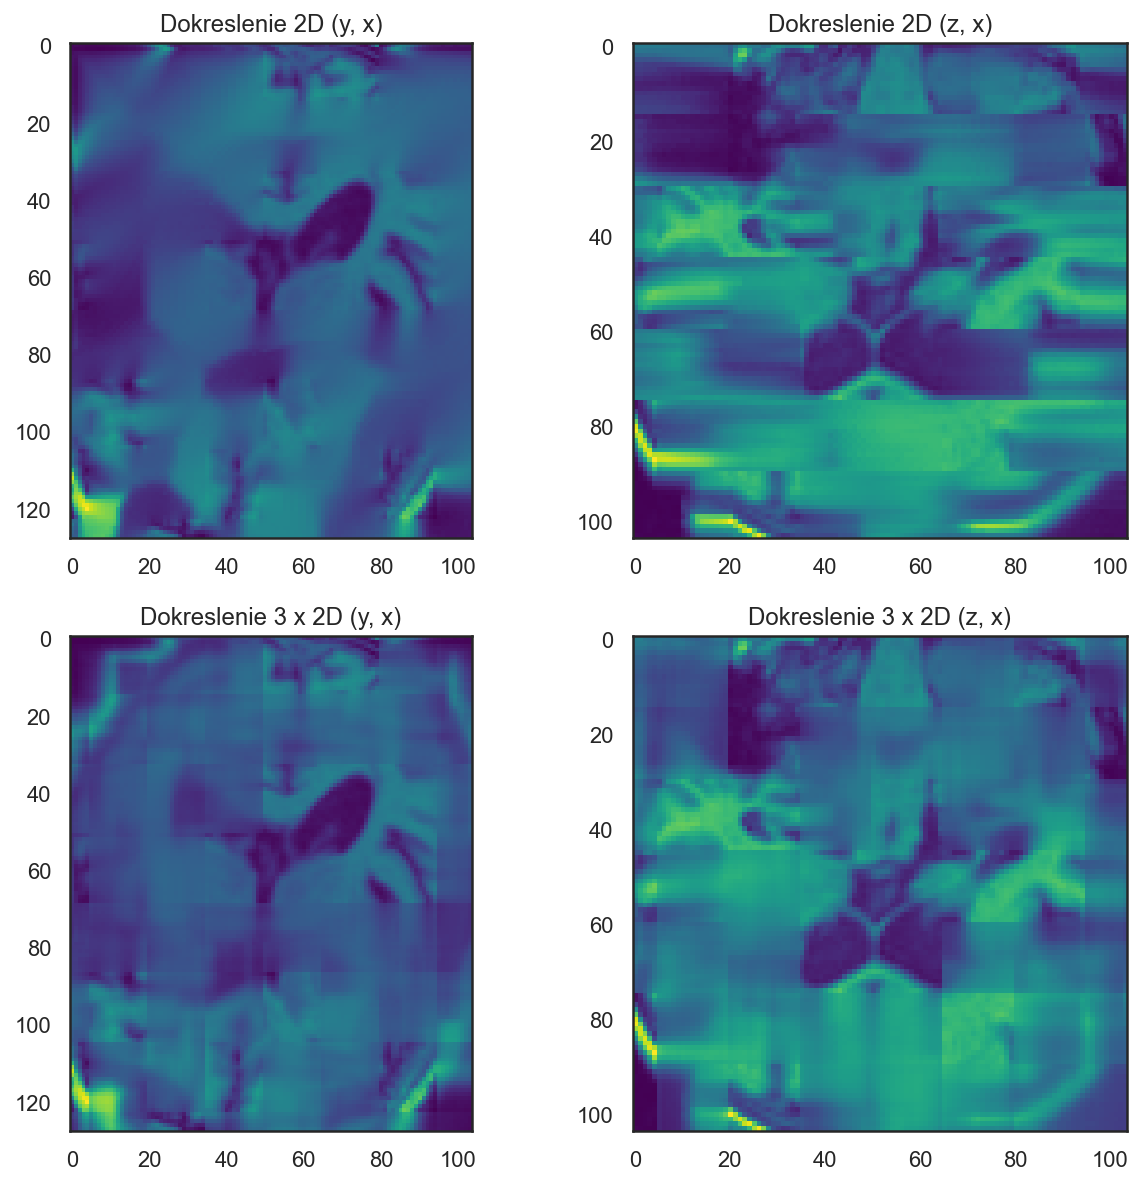
\includegraphics[width=13cm]{assets/images/inpaint_3x_2d.png}
    \caption{Porovnanie 2D dokreslenia (iba v jednej dimenzii) a spriemerovaného 3x 2D dokreslenia (v každej dimenzii). Použitie iba 2D dokreslenia je kvalitné iba v jednej dimenzii a v ostatných je deštruktívne - vytvára ostré hrany. Použitie 3x 2D dokreslenia a spriemerovanie pre každý voxel produkuje celkom dobré dokreslenia po všetkých dimenziách.}
    \label{fig:inpaint_3x_2d}
\end{figure}

Keďže sa pôvodná implementácia RISE prekrýva miesta tak, aby nevznikali ostré hrany medzi zakrytím miestom a pôvodným obrázkon, a teda vznikol plynulý prechod, aj pri dokreslení vytvárame plynulý prechod medzi dokreslením a pôvodným obrázkom (Obr. \ref{fig:inpaint_soft_corners}). Tento prechod je implementovaný nasledovne.
\begin{lstlisting}
    # binary_mask int[z, x, y] - upsized binary mask
    # image float[z, x, y] - original image
    # mask float[z, x, i] - upsizded and interpolated binary mask
    # inpaint_radius int
    inpainted = cv.inpaint(image, binary_mask, inpaint_radius, cv2.INPAINT_TELEA)
    inpainted_blend = image * mask + inpainted * (1 - mask)
\end{lstlisting}

\begin{figure}[h!]
    \centering
    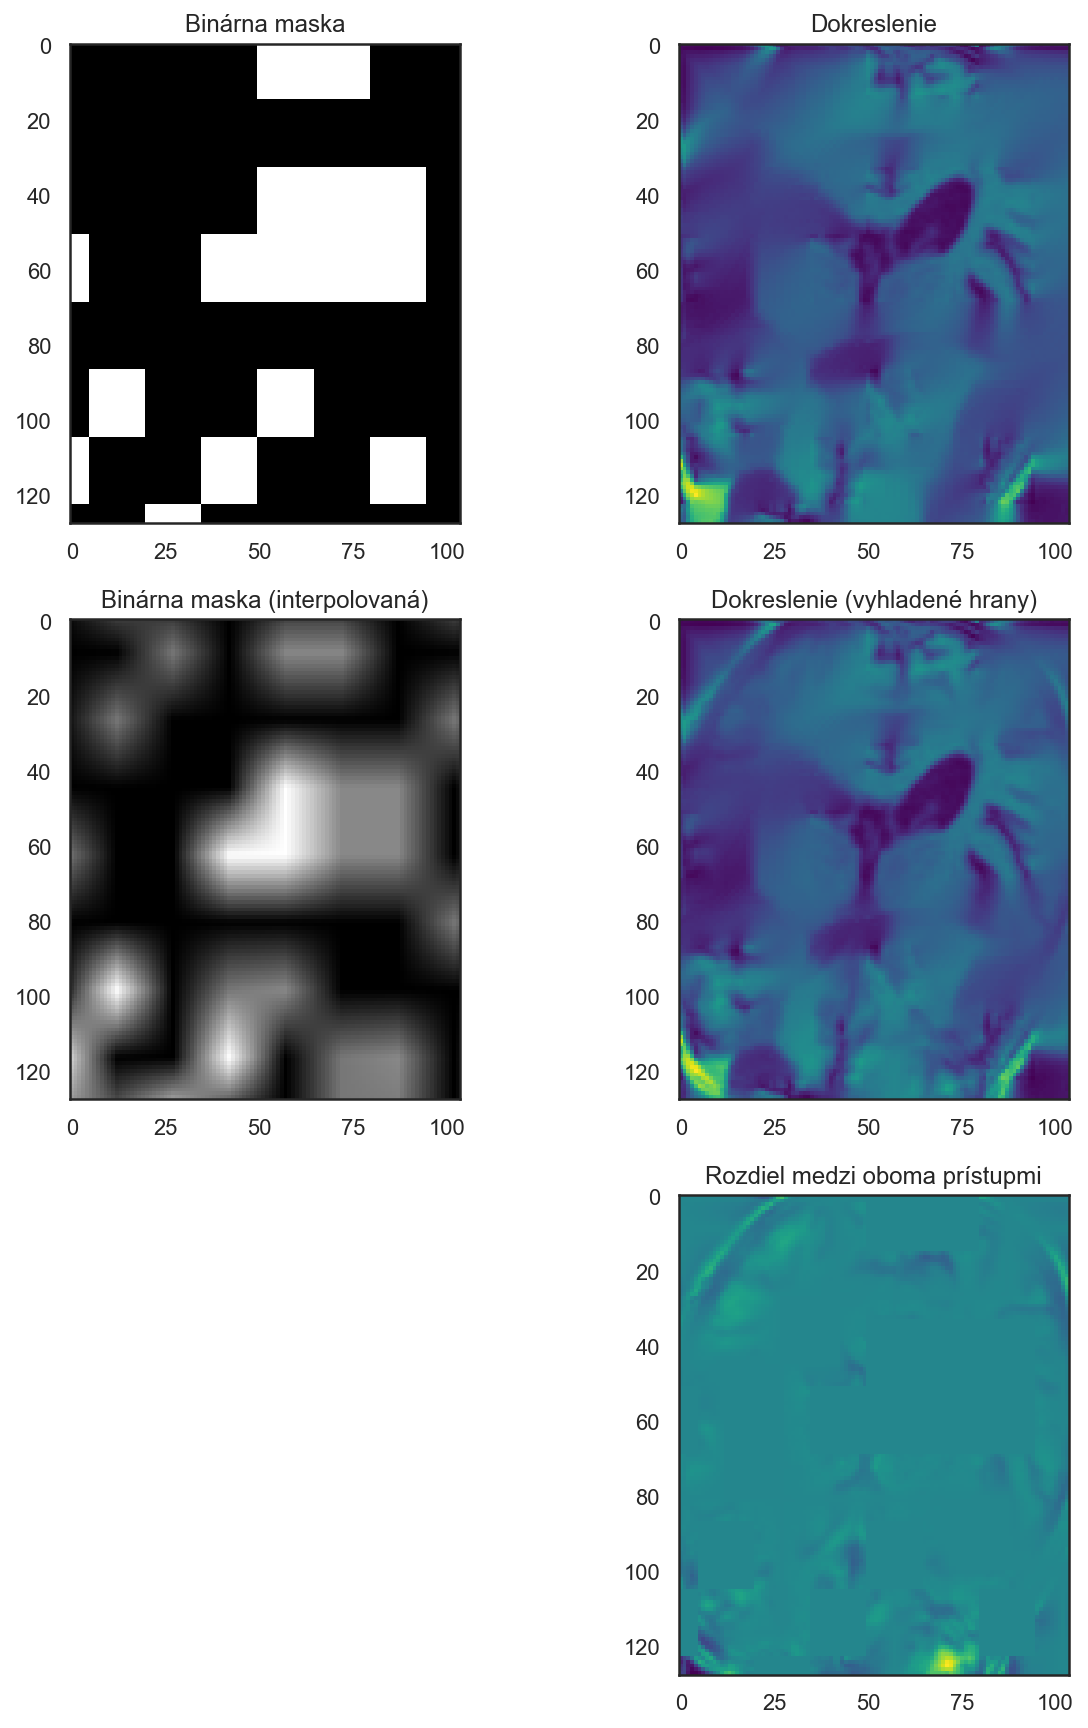
\includegraphics[width=10cm]{assets/images/inpaint_soft_corners.png}
    \caption{Príklad vyhladzovania hrán dokreslenia - splynutie dokreslenia s pôvodným snímkom (štvrtý snímok). Druhý snímok zobrazuje ostré hrany po dokreslení - bez splývania s obrázkom. Piaty snímok zobrazuje rozdiel medzi oboma prístupmi. Môžeme si všimnúť, že na obrázku sí viditeľné miesta, kde sa nachádza prechod na interpolovanej binárnej maske. O tieto miesta (informácie) je dokreslenie s vyhladenými hranami ''bohatšie''.}
    \label{fig:inpaint_soft_corners}
\end{figure}

\begin{figure}[h!]
    \centering
    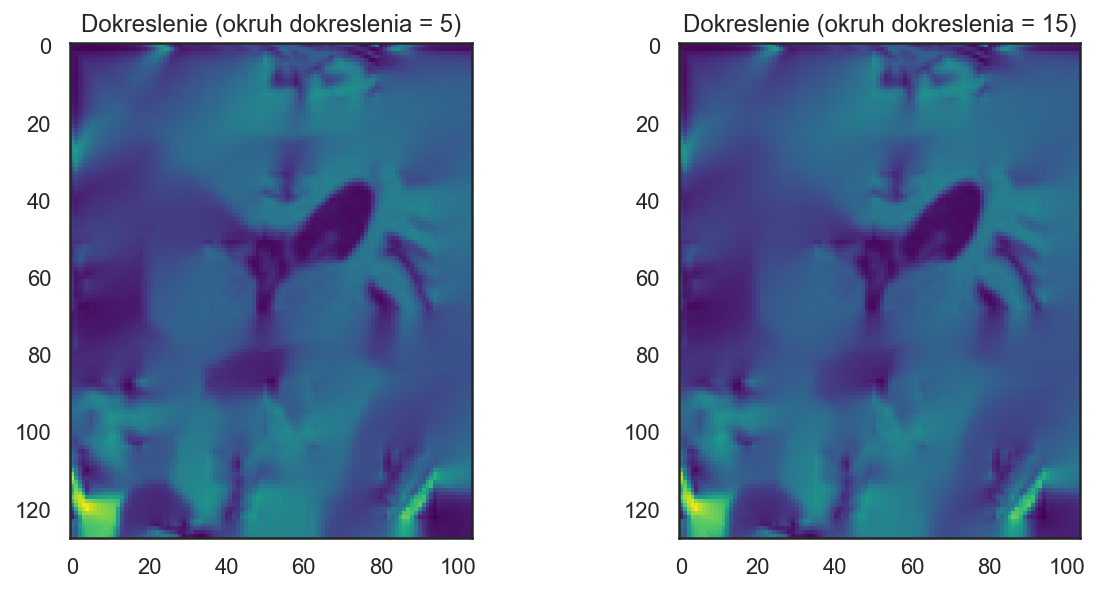
\includegraphics[width=13cm]{assets/images/inpaint_radius.png}
    \caption{Porovnanie okruhov dokreslenia (parameter \textit{inpaint\_radius}), rozdiel vo výsledku nie je veľmi viditelný, avšak s väčśím oruhom dokreslenia je generovanie rádovo pomalšie. (pri generovaní bolo vypnuté splynutie dokreslenia so snímkom aby bol rozdiel aspoň trochu viditeľný)}
    \label{fig:inpaint_radius}
\end{figure}

\paragraph{Prekrytie dokreslenej masky a čiernej masky s obrázkom}

Keďže prekrývam tri rôzne vrstvy - originálny snímok, čiernu masku a dokreslený snímok môžem tieto vrstvy skombinovať v rôznom pomere a tým vytvoriť nový obrázok.

Toto som implementoval zavedením parametrov $b1$ a $b2$ (skratka od slova prechod, angl. blend), ktoré hovoria o pomere medzi originálnym snímkom a dokresleným snímkom, a originálnym snímkom spojeným s dokreslením a čiernou maskou (Obr. \ref{fig:risei_layers}). Pri týchto parametroch platí, že $0 <= b1, b2 <= 1$. Takto zadefinované parametre mi umožňujú vytvoriť zakaskovaný snímok iba s čiernou maskou ($b1 = 0$, $b2 = 1$) či iba s dokreslením ($b1 = 1$, $b2 = 0$).

\begin{figure}[h!]
    \centering
    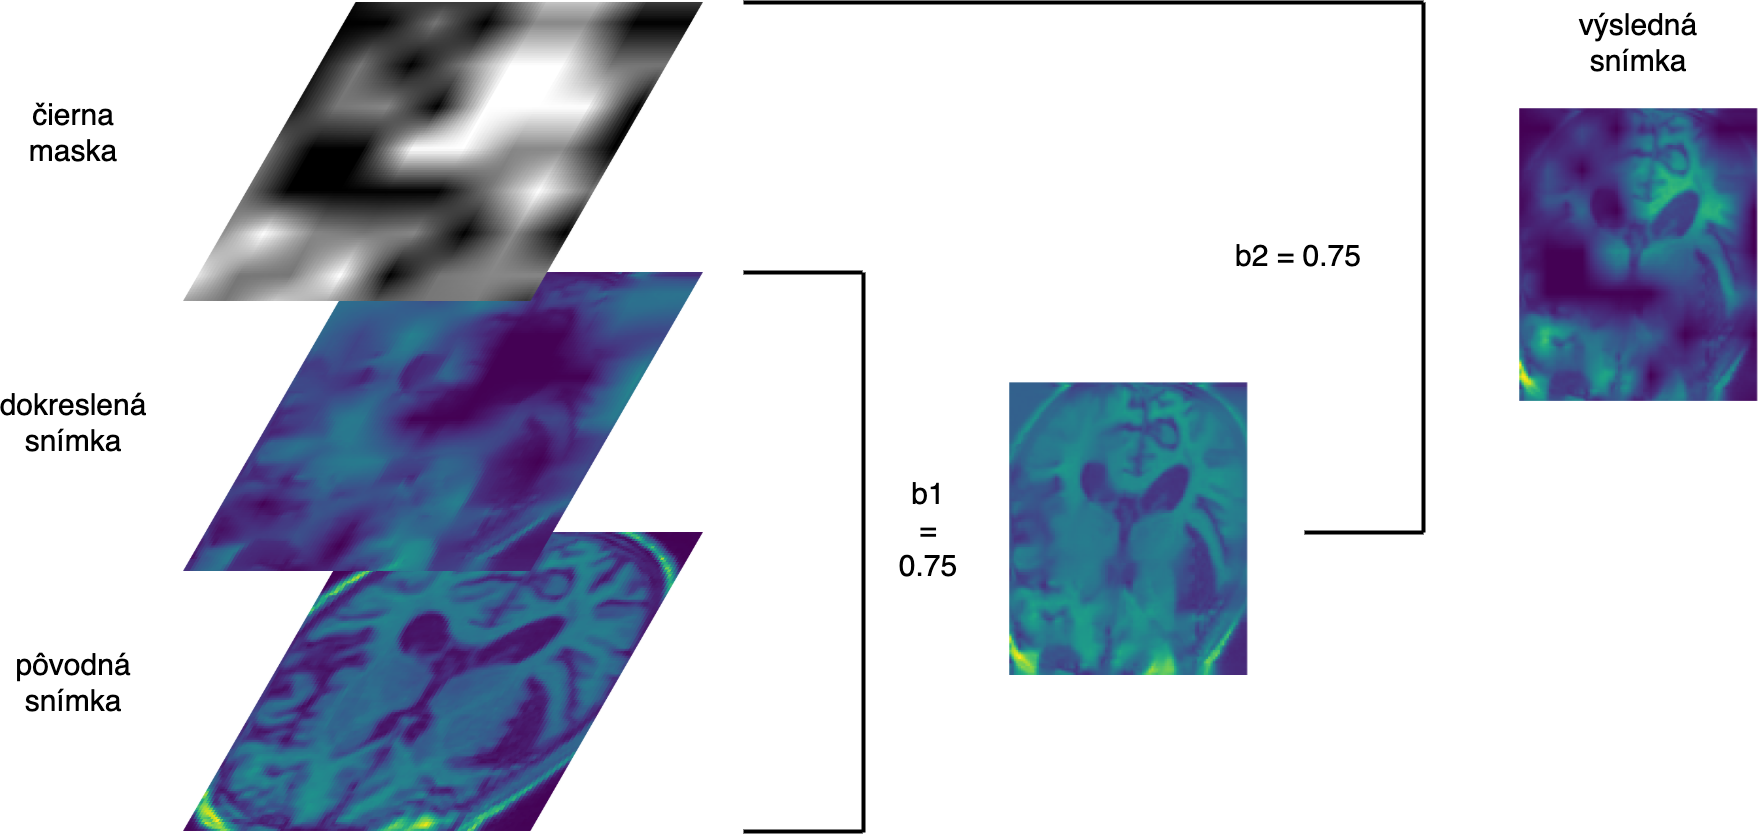
\includegraphics[width=13cm]{assets/images/risei_layers.png}
    \caption{Príklad, ako vyzerá spojenie originálneho snímku, dokresleného snímku a čiernej masky. V diagrame je zobrazený aj výsledok medzikroku spojenia dokresleného snímku a pôvodného snímku. Parametre boli nastavené na $b1 = 0.75$ a $b2 = 0.75$.}
    \label{fig:risei_layers}
\end{figure}

Názov ''čierna'' maska pochádza z pôvodnej implementácie RISE, kde sa obrázok prekrýval čiernou maskou. V našej implementácii neprekrývame farbou, ale hodnotou, tj. ''čierna'' je hodnota $0$ (minimum). Okrem použitia hodnoty $0$, môžeme použiť aj $1$, \textit{priemer} či \textit{medián} (toto je ďaľším hyper-parametrom našej metódy). Zjednodušená (a menej efektívna, v produkčej implementácii sa niektoré inštrukcie nevykonávajú keď \textit{b1} je 0 alebo \textit{b2} je 0) implementácia spojenia jednitlivých vrstiev vyzerá nasledovne.

\begin{lstlisting}
    # image float[z, x, y] - original image
    # inpainted_blend float[z, x, y] - inpainted image
    # mask float[z, x, i] - upsizded and interpolated binary mask
    # b1 float <0, 1>
    # b2 float <0, 1>
    # b2_value string - what value use in "black" mask (min/max/mean/median)

    # merge with inpainted image
    new_image = (1 - b1) * original_image + b1 * inpainted_blend

    value = 0 # black
    if b2_value == 'max':
        value = 1 # white
    elif b2_value == 'mean':
        value = np.mean(original_image)
    elif b2_value == 'median':
        value = np.median(original_image)
    # merge with "black" mask
    new_image = b2 * mask * new_image + (b2 * (1 - mask) * value)
\end{lstlisting}

Kompletný zoznam parametrov metódy RISEI sa nachádza v tabuľke \ref{tab:risei_params}.

\begin{table}[]
    \begin{tabular}{p{0.25\linewidth} | p{0.15\linewidth} | p{0.5\linewidth}}
        \hline
        Názov             & Dátový typ & Popis                                                               \\ \hline
        s                 & int        & Veľkosť strany binárnej 3D matice.                                        \\
        p                 & float      & Pravdepodobnosť, že plocha nebude prekrytá maskou.                        \\
        b1                & float      & Miera prekrytia medzi originálnym snímkom a dokresleným snímkom.          \\
        b2                & float      & Miera prekrytia s ''čiernou'' maskou.                                     \\
        b2\_value         & string     & Hodnota ''čiernej'' masky, môže to byť minimum, maximum, medián, priemer. \\
        in\_paint\_radius & float      & Polomer dokreslenia algoritmom z knižnice OpenCV.                         \\ \hline
    \end{tabular}
    \caption{Zoznam parametrov metódy RISEI.}
    \label{tab:risei_params}
\end{table}

\subsection{Vytvorenie tepelných máp}

Na základe návrhu (Sekcia \ref{sec:risei}) sme implementovali vytváranie tepelných máp. Keďže generovanie tepelnej mapy si vyžaduje vygenerovať veľký počet zamaskovaných snímkov, ktoré v istom momente musia byť všetky uložené v pamäti, generujeme a vyhodnocujeme zamaskované snímky v dávkach (angl. batch). Zdrojový kód nižšie, implementuje vytvorenie jednej tepelnej mapy. Príklad vytvorenej tepelnej mapy uvádzame na obrázku \ref{fig:heatmap_example}.

\begin{lstlisting}
# image_x float[z, x, y, 1] - original image
# masks_count int - how many masks are generated to create a heatmap
# batch_size - how many masks to evaluate on model
# risei_batch_size int - how many masks to generate in one batch
# seed int int - seed for mask generation
# cls_idx int - index of target class in model output vector
# model tf.keras.Model - instance of tensorflow model

risei = RISEI(s=8, p=0.5, b1=0.5, b2=0.5, b2_value='median', in_paint_radius=5)
heatmap = np.zeros(shape=image_x.shape[:3])
batch_count = math.ceil(masks_count / risei_batch_size)
weights = 0

for batch_idx in range(batch_count):
    batch_masks_count = min(risei_batch_size, masks_count - batch_idx * risei_batch_size)
    # reshape input for RISEI since it works with [z, y, x] shape
    # batch_x float[z, x, y] - images to evaluate with masks already applied
    # masks float[z, x, y] - interpolated binary masks (so we know which places we inpainted or masked)
    batch_x, masks = risei.generate_masks(batch_masks_count, image_x.reshape(image_x.shape[:3]), seed=seed)
    y_pred_batch_x = model.predict(batch_x.reshape((-1, *image_x.shape)), batch_size=batch_size)

    for mask, y_pred in zip(masks, y_pred_batch_x):
        # invert the mask, since 1 is for no masking
        # y_pred is the activation for the input masked image on last layer (softmax)
        heatmap = heatmap + y_pred[cls_idx] * (1 - mask)
        weights += y_pred[cls_idx]

heatmap = heatmap / weights
\end{lstlisting}

\begin{figure}[h!]
    \centering
    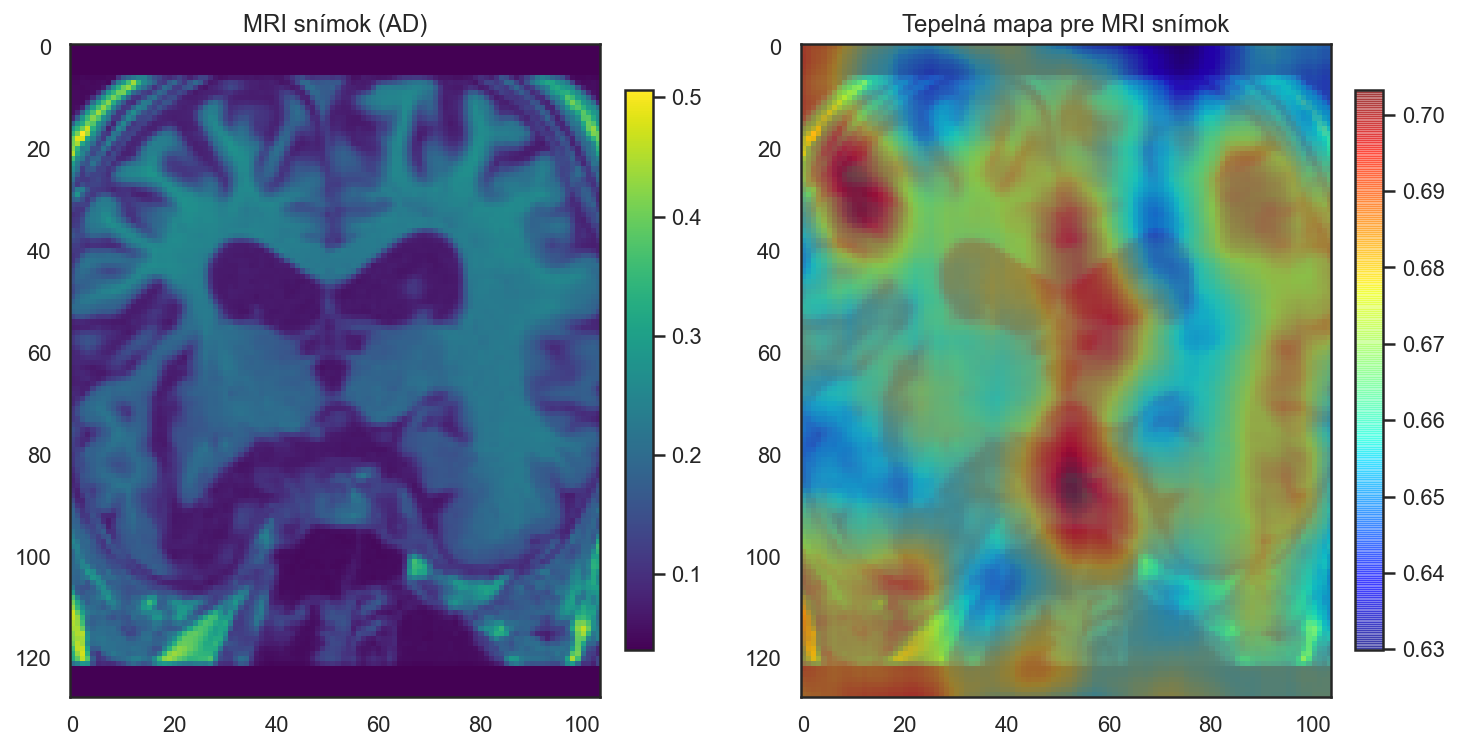
\includegraphics[width=10cm]{assets/images/heatmap_example.png}
    \caption{Príklad vytvorenej tepelnej mapy (vpravo) k MRI snímku (vľavo). Mierka vujadruje priemernú mieru aktivácie pre daný voxel.}
    \label{fig:heatmap_example}
\end{figure}

\subsection{Vyhodnotenie tepelných máp}

Zatiaľ sme implementovali, podľa návrhu riešenia (Sekcia \ref{sec:evaluation_design_method_quality}), iba metriky \textit{insertion} a \textit{deletion}.

\subsubsection{Metriky insertion \& deletion \label{sec:insertion_deletion}}

Tieto metriky fungujú tak, že postupne odstraňujeme/pridávame pixely z obrázku a tieto obrázky vkladáme do modelu a zaznamenávame si aktiváciu na poslednej vrstve pre predikovanú triedu. V prípade obrázkov, a teda dvojrozmerných dát je to ešte výpočtovo zvládnutelné, avšak v prípade trojdimenzionálnych rádiologických simkov to už môže byť problém. Naše vstupné snímky majú po zmenšení rozmer \textit{[104, 128, 104]}, čiže ak aby sme odstraňovali zo snímku po jednom voxeli, museli by sme vykonať \textit{1 384 448} evaluácii pomocou nášho modelu (čo trvá niekoľko hodín, aj pri evaluovaní v maximálnych možných dávkach vzhľadom na pamäť grafickej karty). Preto sme sa rozhodli, že budeme pridávať po $n$ (~100) voxeloch v každom kroku. V prípade metódy insertion vkladáme do snímku plného núl (môžeme prípadne aj jednotiek). Keďže kód je rozsiahlejší, uvedieme len pseudokód.

\begin{lstlisting}
method = 'insertion'
step_size = 150 # how many voxels to insert/delete in one evaluation
image_x, image_y = get_image()
image_y_pred = model.predict(image_x)
heatmap = get_heatmap()
voxels = get_ordered_voxels_by_heat(heatmaps)
sequence = get_images_sequence(voxels, step_size) # create a sequence from images where each next image has n inserted/deleted voxels
y_pred = []

for batch_x, batch_y in sequence:
    batch_y_pred = model.predict(batch_x)
    for y in batch_y_pred:
        y_pred.append(y)

auc = metrics.auc([i * step_size for i in range(len(y_pred))], y_pred) / get_voxels_count(image_x)
\end{lstlisting}

\section{Model na detekciu Alzheimerovej choroby na základe MRI snímkov}

V tejto sekcii popíšem impelentáciu, z ktorého predikcií budeme vytvárať tepelné mapy. Náš model - neuónovú sieť sme sa rozdhodli implementovať v knižnici Tensorflow (v2.3.0). Naším cieľom nie je natrénovať najlepší model na dekekciu Alzheimerovej choroby, ale model ktorý je použiteľný na overenie nami narvhnutej metódy. Preto nevykonáme komplexnejšie prístupy k detekcii Alzheimerovej chorby, ktoré sme popísali v analýze (Sekcia \ref{sec:nn_ad_prediction}), ako je napríklad učenie prenosom pomocou autoenkodéra.

\subsection{Dátová sada}

Použili sme dátovú sadu ADNI. Ako vstup modelu je celý MRI snímok (tj. všetky tri dimenzie), nepoužívame žiadné ine údaje z dátovej sady ADNI, ako napríklad demografické údaje a pod. keďže model plánujeme používať iba na vytváranie tepelných máp pre vstupné snímky. 

V dátovej sade sa nachádza celkom 502 MRI snímkov, z toho 311 pacientov s Alzheimerovou chorobou (AD) a 191 bez (CN). Dátovú sadu máme teda nevyváženú a model môže začať preferovať jednu triedu. Na predíjdenie tomuto javu existuje niekoľko techník, napríklad nadvzorkovanie (angl. oversampling) alebo podvzorkovanie (angl. undersampling) kedy sa doplní synetetickými minoritná trieda, alebo sa odstránia nejaké pozorovania z majoritnej triedy. My sme sa však rozhodli nastaviť predikovaným triedam váhy, ktoré sú zohladnené v chybovej funkcii, taktiež sme nainicializovali chybu \footnote{\url{https://www.tensorflow.org/tutorials/structured\_data/imbalanced\_data\#optional\_set\_the\_correct\_initial\_bias}} pre neuróny na poslednej vrstve aby reflektovala to, že triedy sú nevyvážené.

Dátovú sadu sme náhodným výberom rozdelili na trénovaciu a testovaciu v pomere 80/20. Validačnú sadu sme nerobili, pretože máme málo dát a neplánujeme robiť veľké hľadania optimálnych hyper-parametrov. V budúcnosti možno zvážime vykonanies krížovej validácie (angl. cross validation) pri trénovaní. Aj po rozdelení sa nám podarilo zachovať pôvodný pomer medzi triedami -- 62/38 (Obr. \ref{fig:dataset_classes}).

\begin{figure}[h!]
    \centering
    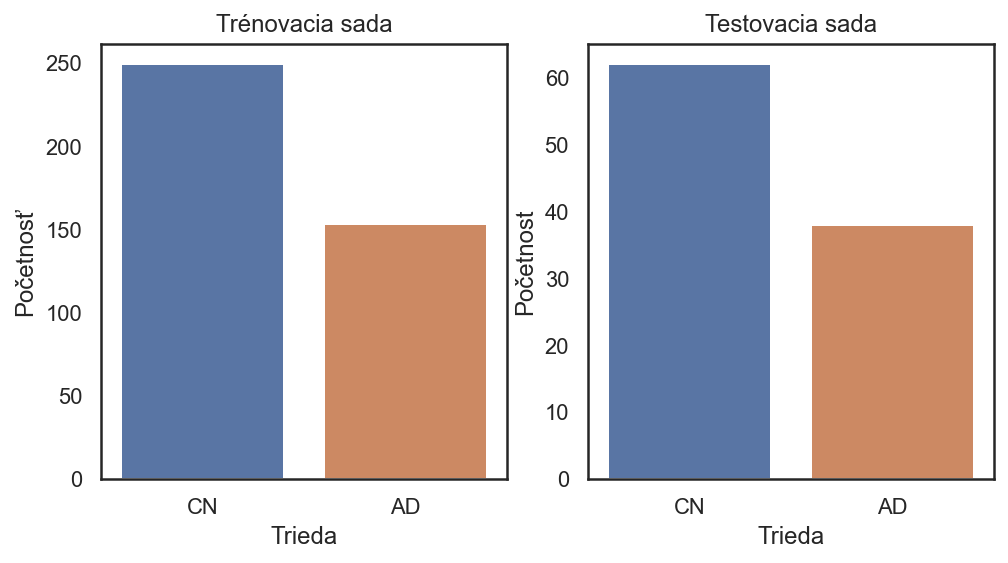
\includegraphics[width=10cm]{assets/images/dataset_classes.png}
    \caption{Početnosť tried medzi trénovacou a testovacou sadou - je zrejmá prevaha triedy AD.}
    \label{fig:dataset_classes}
\end{figure}

\subsubsection{Predspracovanie}

MRI snímky boli predspracované štandardnou postupnosťou nástroja freesurfer, avšak nevykonali sme odstránenie lebky z MRI snímkov.
Okrem iného sme vykonali:

\begin{itemize}
    \item Upravenie vstupných snímkov na rovnakú veľkosť 104 x 128 x 104 voxelov. \citeauthor*{esmaeilzadeh2018end} upravili vstupné snímky na veľkosť 116 x 130 x 83, k týmto číslam sme sa pokúsili priblížiť. Pomer veľkostí dimenzií ale nemáme rovnaký, aj z dôvodu, že sme nevykonali odstránenie lebky zo vstupných snímkov.
    \item Štandardizáciu vstupných dát (preškálovanie na rozsah $<0, 1>$) nasledovným vzorcom: $\frac{(image\_x - images\_min])}{(images\_max - images\_min)}$.
\end{itemize}

\subsubsection{Augmentácie}

Keďže máme málo dát, rozhodli sme sa dáta augmentovať (Obr. \ref{fig:augmentations}). Dáta náhodne augmentujeme v každej dávke (angl. batch). Implementovali sme nasledovné augmentácie:

\begin{itemize}
    \item Vymenenie hemisfér mozgu (\citeauthor*{esmaeilzadeh2018end}) s pravdepodobnosťou 50\%
    \item Náhodná rotácia o 0 až 5 stupňov s pravdepodobnosťou 20\%
    \item Náhodné priblíženie do 80\% veľkosti snímku s pravdepodobnosťou 20\%
    \item Náhodné gaussovské rozmazanie (max $sigma = <0.85, 1>$) s pravdepodobnosťou 20\%
    \item Náhodný gaussovský šum pravdepodobnosťou 20\%
\end{itemize}

\begin{figure}[h!]
    \centering
    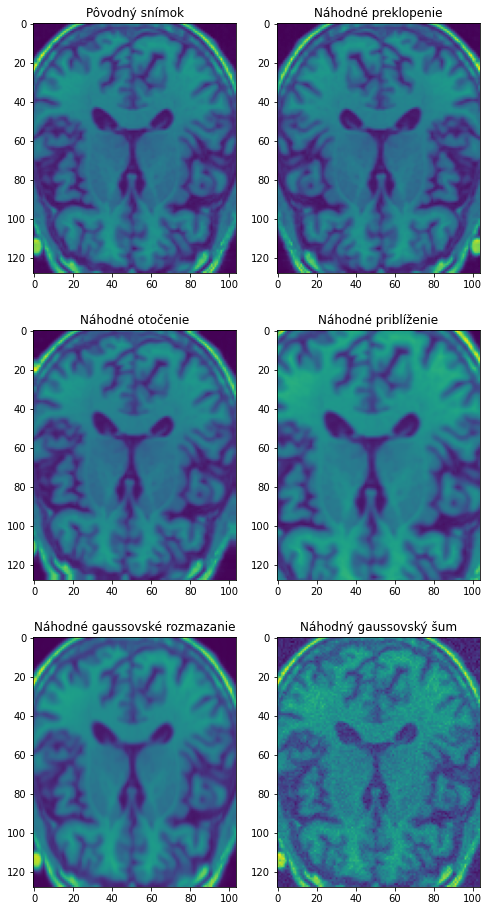
\includegraphics[width=10cm]{assets/images/augmentations.png}
    \caption{Príklady aplikácie implementovaných augmentácií.}
    \label{fig:augmentations}
\end{figure}

\subsection{Model}

Rozhodli sme sa implementovať a porovnať niekoľko architektúr neurónových sietí.

\paragraph{3D konvolučná neurónová sieť od \citeauthor*{esmaeilzadeh2018end}} Túto neurónovú sieť sme sa rozhodli implementovať, pretože jej autori pomocou nej dosiahli veľmi slušné výsledky (94.1\% presnosť). Implementovali sme jednoduchšiu verziu, ktorá dosahovala lepšie výsledky, opísali sme ju v sekcii \ref{sec:nn_ad_prediction}. Táto neurónová sieť ma celkovo \textit{2 899 778} parametrov.

\paragraph{2D ResNet a 3D ResNet} Keďže reziduálne neúronové siete dosahujú pri klasifikačných úlohách nad obrazovými dátami veľmi dobre výsledky vyskúšame aj tieto architektúry. V prípade 2D ResNetu-u používame 2D konvolúcie, tie nám budú fungovať aj napriek tomu, že máme 3D dáta. Vstup do 2D ResNet-u je tiež 3D matica, ktorej tretia dimenzia býva o obvykle o dĺžky 1 alebo 3 (RGB), v našom prípade bude o veľkosti poslednej dimenzie snímku. Rozmery vstupných dát pre 2D ResNet budú $[104, 128, 104]$ a pre 3D ResNet $[104, 128, 104, 1]$. Za konvolučné vrstvy a globálnu združovaciu vrstvu sme pripojili dve plne prepojené vrstvy s 512, 256 a 128 neurónami a aktiváciou \textit{ReLU}, následne už nasleduje iba posledná vrstva s aktiváciou \textit{softmax}. Tieto neurónové siete majú celkovo \textit{12 689 602}, resp. \textit{34 356 354} parametrov.

Do neurónových sietí sme ešte pridali dropout a dávkovú normalizáciu (angl. batch normalization). Dropout sme pridali pred plne prepojené vrstvy. Dávkovú normalizáciu sme pirdali v konvolučných vrstvách pred aplikovaním nelinearity, tak ako je to odporučené od \citeauthor*{ioffe2015batch} v \textit{Batch Normalization: Accelerating Deep Network Training by Reducing Internal Covariate Shift}. Na poslednej vrstve sa nachádzajú dva neuróny s aktiváciou \textit{softmax}.

\subsection{Trénovanie}

Pri trénovaní sme použili:

\begin{itemize}
    \item kategorickú entropiu (angl. categorical crossentropy) ako chybovú funkciu s podporou pre nevyvážené triedy (tj. táto funkcia brala ohľad na váhy tried, ktoré sme nastavili),
    \item optimizér Adam s prevolenými nastaveniami,
    \item exponenciálne tlmenie rýchlosti učenia (angl. learning rate decay), $0,96$ každých 25 epoch
    \item skoré zastavenie trénovania ak sa metrika AUC (plocha pod krivkou) nezlepšila za posledných 50 epoch,
    \item veľkosť dávky (angl. batch size) -- 10 (vždy tak, aby sme naplno využili pamäť grafickej karty),
    \item $l2$ regularizáciu (rovnako ako \citeauthor*{esmaeilzadeh2018end}).
\end{itemize}

Trénovali sme iteratívne, začali sme obyčajným modelom a postupne sme pridávali augmentácie, dávkovú normalizáciu, dropout a regularizáciu pričim sme postupne dolaďovali parametre. Najlepšie výsledky sme dosiahli s architektúrou 3D ResNet s presnosťou 80\% (Tabuľka \ref{tab:model_training_results}). Nepodarilo sa nám nám teda priblížiť k výsledkom analyzovaných prác.

\begin{landscape}
    \begin{table}[]
        \centering
        \begin{tabular}{l|rrr|rrr|rrr|}
            \cline{2-10}
            \multirow{2}{*}{}    & \multicolumn{3}{c|}{3D CNN} & \multicolumn{3}{c|}{3D ResNet} & \multicolumn{3}{c|}{2D ResNet} \\ \cline{2-10} 
            &
            \multicolumn{1}{c|}{Acc.} &
            \multicolumn{1}{c|}{Sens.} &
            \multicolumn{1}{c|}{Spec.} &
            \multicolumn{1}{c|}{Acc.} &
            \multicolumn{1}{c|}{Sens.} &
            \multicolumn{1}{c|}{Spec.} &
            \multicolumn{1}{c|}{Acc.} &
            \multicolumn{1}{c|}{Sens.} &
            \multicolumn{1}{c|}{Spec} \\ \hline
            \multicolumn{1}{|l|}{Baseline}             & 0.71    & 0.76    & 0.63    & 0.71     & 0.79     & 0.57     & 0.67     & 0.77     & 0.50     \\
            \multicolumn{1}{|l|}{+ Augmentácie}        & 0.67    & 0.68    & 0.66    & 0.69     & 0.84     & 0.45     & 0.76     & 0.90     & 0.52     \\
            \multicolumn{1}{|l|}{+ Batch Norm}         & 0.75    & 0.77    & 0.71    & 0.80     & 0.85     & 0.71     & 0.77     & 0.89     & 0.58     \\
            \multicolumn{1}{|l|}{+ Dropout}            & 0.75    & 0.76    & 0.74    & 0.74     & 0.94     & 0.42     & 0.77     & 0.85     & 0.63     \\
            \multicolumn{1}{|l|}{+ Regularizácia (l2)} & 0.71    & 0.70    & 0.71    & 0.79     & 0.87     & 0.66     & 0.78     & 0.89     & 0.61    
        \end{tabular}
        \caption{\textbf{Výsledky trénovania.} Acc. = presnosť (angl. Accouracy), Sens. = senzitivita (angl. Sensitivity), Spec. = Špecificita (angl. Specificity)}
        \label{tab:model_training_results}
    \end{table}
\end{landscape}

Oproti \citeauthor*{esmaeilzadeh2018end}, ktorí dosiahli presnosť až 94\%, sme dosiahli presnosť len 72\% avšak sme mali menej dát (o 339 pozorovaní menej), neodstraňovali sme zo snímkov lebku a nepoužili sme pri klasifikácii vek pacienta. Avšak robili sme viac augmentácií, a po ich pridaní sa úspešnosť modelu zhoršila (Obr. \ref{fig:3d_cnn_training}) (ale následne sa už iba zlepšovala), je teda možné, že niektoré augmentácie sú nekorektné a deštruktívne. V ďaľších experimentoch by sme mali pridávať augmentácie po jednej. Aj po pridaní veľmi slabej regularizácie, sa úspešnosť modelu zhoršila. V prípade 2D a 3D ResNet architektúr sa nám podarilo dosiahnuť lepšie výsledky, avšak v ich prípade sa sieť neskôr začala pretrénovávať (Obr. \label{ref:2d_3d_res_net_training}
) aj napriek použitej regularizácii, čo môže naznačovať, že sú tieto architektúry na náš problém príliš komplexné.

Možné vylepšenia (zoradené podľa subjektívneho pomeru úsilie/vplyv):
\begin{itemize}
    \item Pridávať augmentácie postupne a vyhodiť tie deštruktívne.
    \item Menej ''agresívne'' augmentácie.
    \item Odstránenie lebky zo snímkov.
    \item Nájsť a použiť viac dát.
    \item Krížová validácia v prípade väčšieho nastavovania hyperparametrov.
    \item Učenie prenosom pomocou autoenkodéra \cite{hosseini2016alzheimer}.
\end{itemize}

\begin{figure}[h!]
    \centering
    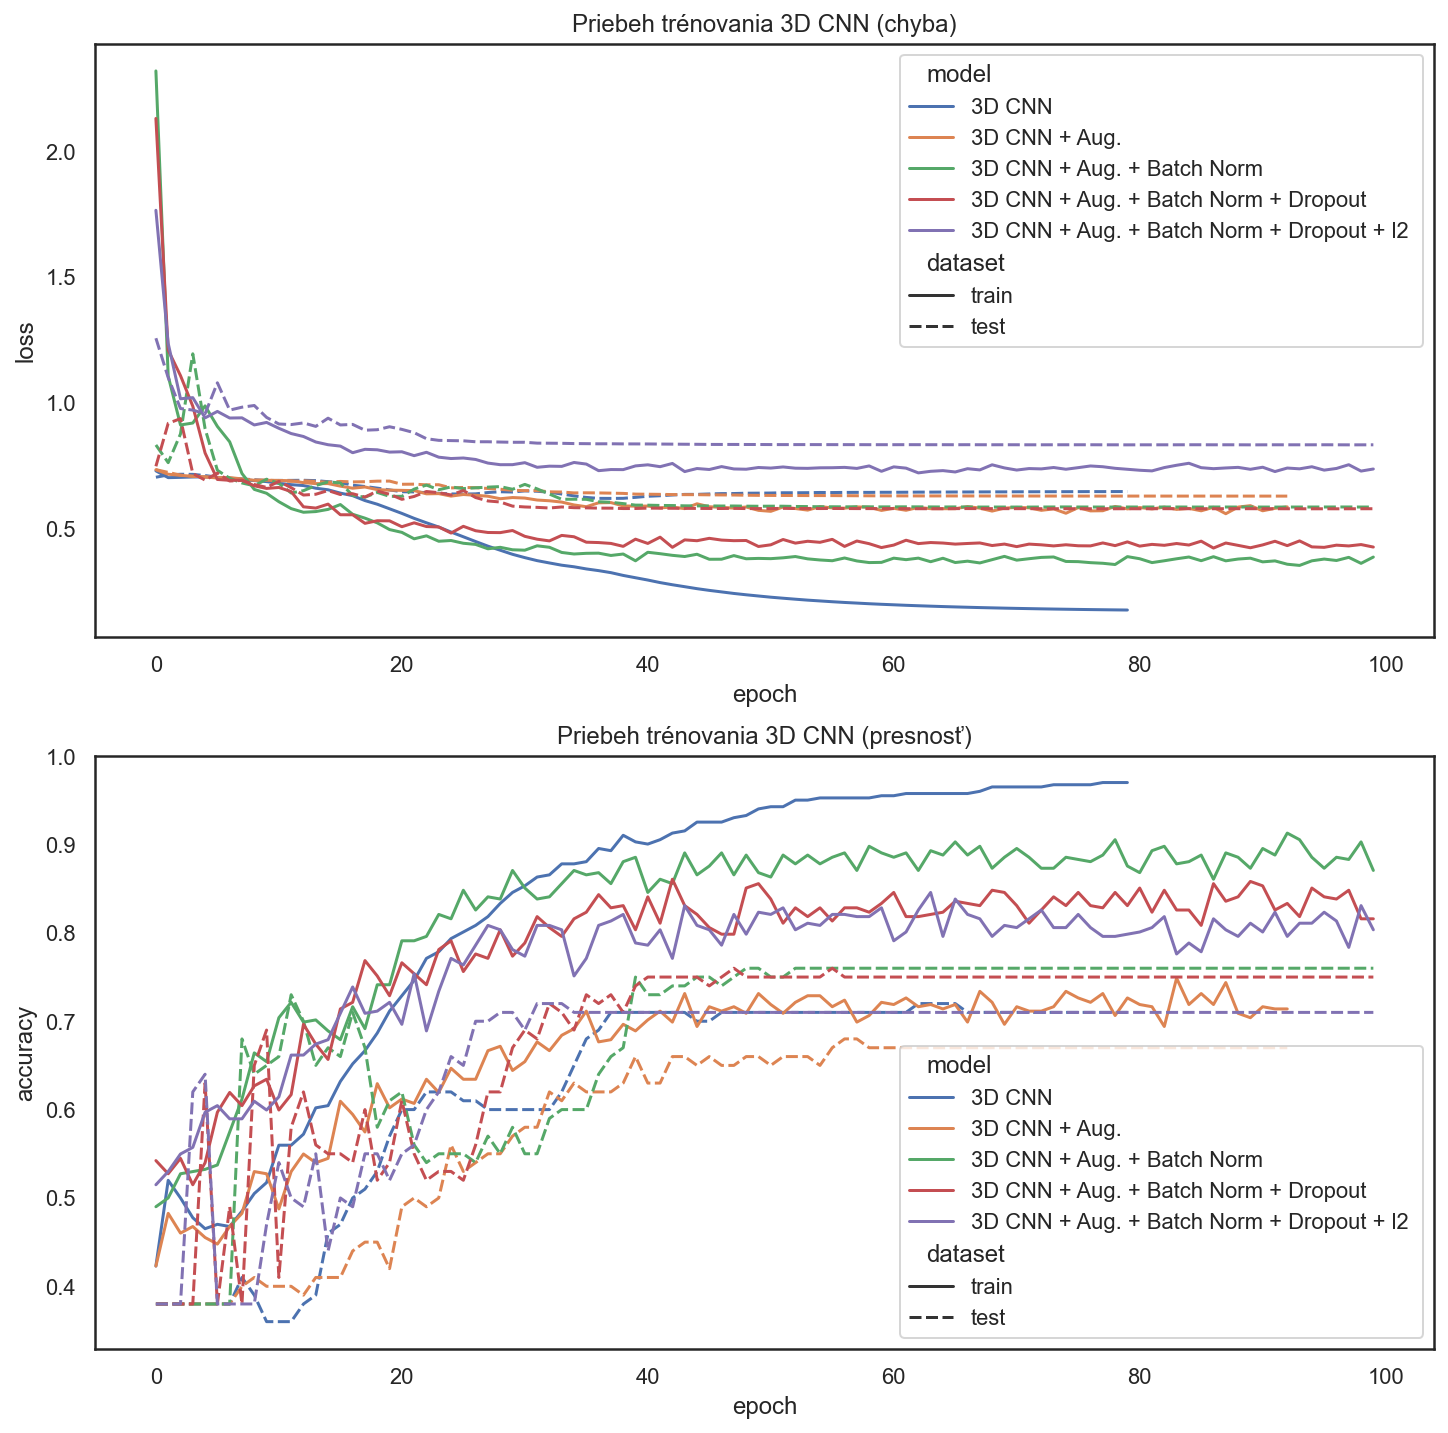
\includegraphics[width=14cm]{assets/images/3d_cnn_training.png}
    \caption{Priebeh trénovania 3D konvolučnej neurónovej siete, čím viac sme pridali regularizácie (l2 alebo dropout) tým sme dosiahli horšie výsledky. Po pridaní augmentácií sa úspešnosť modelu zhoršila, avšak následne sa už iba zlepšovala.}
    \label{fig:3d_cnn_training}
\end{figure}

\begin{figure}[h!]
    \centering
    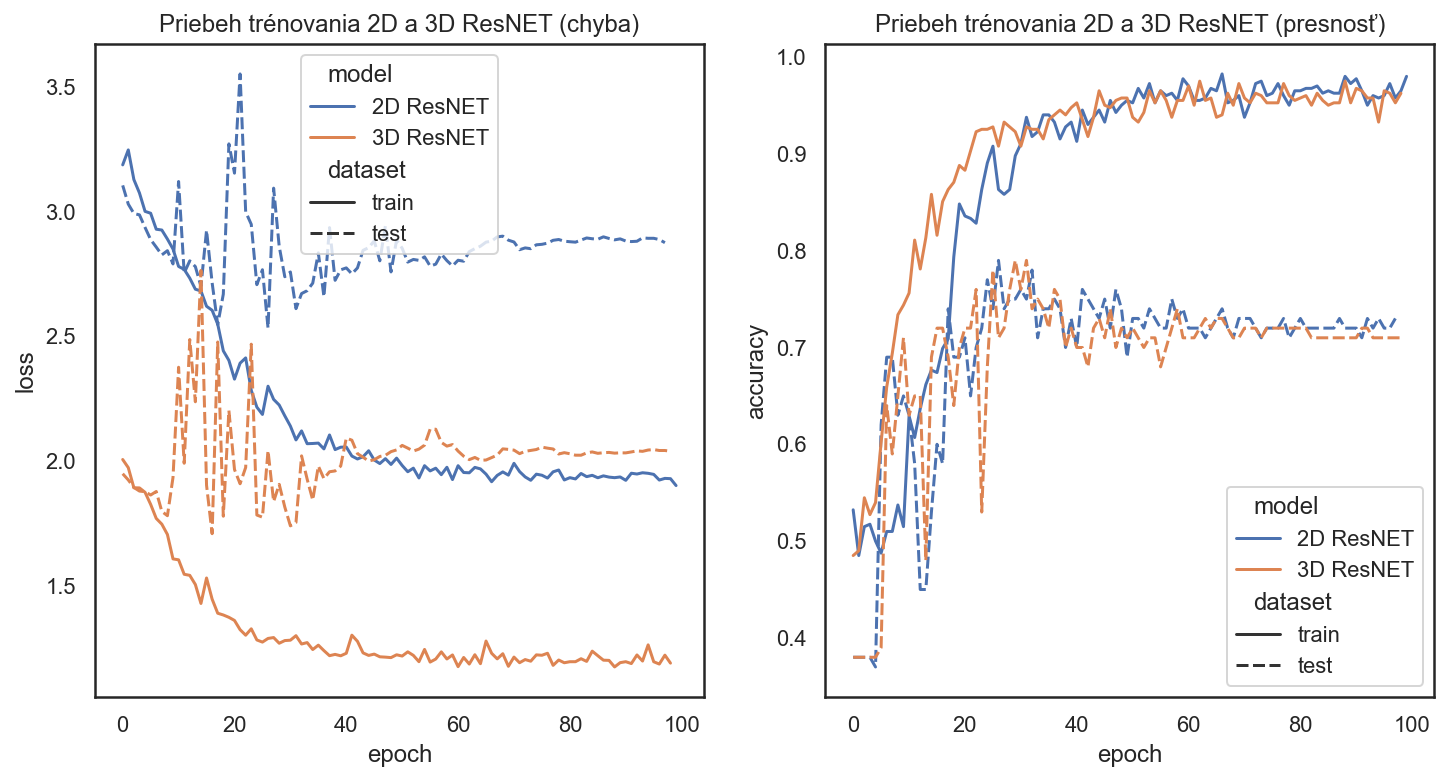
\includegraphics[width=14cm]{assets/images/2d_3d_res_net_training.png}
    \caption{Priebeh trénovania 2D a 3D ResNet neurónovej siete. V oboch prípadoch sme použili dropout aj regularizáciu. Od približne 30-tej epochy sa neurónová sieť začala pretrénovávať, aj napriek regularizácii. Ako vylepšenie je možné skúsiť silnesjšiu regularizáciu (väčšiu hodnotu l2 a dropout), ak ani to nepomôže, je možné, že architektúra je príliš komplexná náš problém (neurónová sieť je príliš hlboká). Môžeme ďalej skúsiť odstrániť jednu plne prepojenú vrstvu alebo znížiť počet neurónov v týchto vrstvách.}
    \label{fig:2d_3d_res_net_training}
\end{figure}

\section{Záver}

V tejto kapitole sme opísali ako sme implementovali nami navrhovanú metódu a spôsob jej overenie. Opísali sme implemetáciu kľúčových prvkov (generovanie masiek a vytvorenie tepelnej mapy) navrhovanej metódy RISEI a jej hyper parametre. Rovnako sme opísali aj implementáciu neurónovej siete, architektúru, spôsob trénovania a použitú dátovú sadu. Metódu RISEI sa nám podarilo implementovať a je ich možné použiť v experimentoch. Podarilo sa nám natrénovať niekoľko architektúr neurónových sietí, pričom sme indetifikovali možné príčiny (a navrhli k nim riešenia) výsledkov, ktoré dosahujú. Každopádne výsledky považujeme za postačujúce pre prvé experimenty navrhovanej metódy RISEI.


    % Verification
    \clearpage\null
    \chapter{Overenie riešenia}

Keďže sme natrénovali viacero modelov, a metóda RISEI má veľké množstvo parametrov zvolili sme nasledovnú stratégiu pri overovaní riešenia, tak aby sme nemuseli overovať všetky možné kombinácie parametrov/architektúr a dokázali vykonať všetky navrhnuté experimenty (Sekcia \ref{sec:design_experiments}) v stanovenom čase.

\begin{enumerate}
    \item Výber architektúry neurónovej siete na ktorej budeme overovať metódu RISEI a porovnávať ju z ostatnými. \textit{Ktorý model je najvhodnejší pre navrhnutú metódu?}
    \item Overenie metódy RISEI. \textit{Dávajú výsledky z navrhnutej metódy zmysel a nie sú náhodné?}: 
         \begin{itemize}
             \item Overenie stability tepelných máp.
             \item Overenie kvality tepelných máp (metriky \textit{insertion} a \textit{deletion}).
         \end{itemize}
    \item Porovnanie kvality tepelných máp s metódou RISE (s doimplementovanou podporou pre 3D snímky) - \textit{je to metóda, ktorá je metóde RISEI najbližšie, je navrhnutá metóda lepšia?}
    \item Overenie správnosti tepelných máp a porovnanie s inými metódami - GradCAM, Guided Backprop, Guided GradCAM. \textit{Sú tepelné mapy nie len kvalitné, ale dávajú zmysel v kontexte anatómie mozgu? Ako sú na tom iné metódy?}
\end{enumerate}

\paragraph{Adresovanie náhodnosti metódy RISE pri porovnávaní dvoch roznych modelov}

Keďže vygenerované masky sú náhodné, pri porovnávaní dvoch metód (kombinácii rôznych parametrov metódy RISEI) generujeme rovnaké binárne masky pre každý i-ty snímok, tj. zakryté pozície sú rovnaké, rôzna je len hodnota zakrytia. Vygenerované binárne masky pre jednotlivé snímky v testovacej sade sú stále náhodné (a teda aj medzi sebou rôzne). Rovnaké sú len binárne masky pre dve rôzne generovania masiek pre ten istý snímok v testovacej sade. Takto dosiahneme kvalitnejšie výsledky, pretože žiadna metóda nebude mať výhodu, že náhodou zakryla rôzne časti snímky lepšie a teda bude dôležité ako ich zakryla.

\section{Experimenty}

\subsection{Výber architektúry neurónovej siete pre ďaľšie experimenty \label{sec:experiment_rise_various_architectures}}

V tomto experiemnte sme porovnali metódu RISE na nami natrénovaných modeloch s cieľom vybrať jeden z nich pre ďaľšie experimenty (keďže experimenty sú časovo náročné, nechceme ich robiť na všetkých modeloch). Vybrali sme najlepšie natrénované modely pre každú architektúru (Tabuľka \ref{tab:model_training_results}). Použili sme nami implementovanú metódu RISEI pričom sme nastavili jej parametre tak, aby fungovala ako metóda RISE.
Parametre sme nastavili nasledovne: $s = 8$, $p = 1/3$, $b1 = 0$, $b2 = 1$ (opis parametrov sa nachádza v tabuľke \ref{tab:risei_params}). Na vytvorenie tepelnej mapy sme vygenerovali 1024 masiek. Pri vyhodnocovaní metrík insertion a deletion sme nastavili veľkosť kroku na 2500 voxelov (takto trvalo vyhodnotenie tepelnej mapy ~3 minúty). Vybrali sme 25 náhodných snímkov z testovacej sady (13 AD, 12 CN), generovanie a vyhodnotenie tepelných máp k nim trvalo približne ~1 hodinu. 

Najlepšie výsledky sme dosiahli na architektúre 3D CNN (Tabuľka \ref{tab:experiment_rise_various_architectures}). Je dôležité si ale uvedomiť, že na vyhodnotenie metrík \textit{insertion} a \textit{deletion} z vytvorenej tepelnej masky sa používa model samotný - zo snímky sú pridávané/odoberané voxely pričom sa sleduje sa zmena predikcie modelu. Môže nastať teda situácia, že dva rôzne modely vytvoria dve identické tepelné mapy, pričom výsledná hodnota metriky bude rozdielna. Na základe týchto metrík teda nemôžeme tvrdiť, že jeden model vytvára lepšie tepelné mapy ako druhý. Metrika \textit{insertion} a \textit{deletion} nie je teda vhodná na takéto porovnanie dvoch rôznych modelov medzi sebou.
Dobrým signálom by bolo ak by hodnota metriky \textit{insertion} bola väčšia ako metriky \textit{deletion}, takto to nie je ani u jedného z modelov (najbližšie má k tomu 3D CNN). Aj kvôli tomuto sme vybrali do ďaľších experimentov model 3D CNN, zároveň na základe jeho špecificity a senzitivity môžeme tvrdiť, že nepreferuje ani jednu z tried - čo u iných modeloch tak nie je (tie preferujú AD pozorovania). Taktiež je tento model jednoduchší.

\begin{table}[]
    \centering
    \begin{tabular}{cl|r|r|r|}
        \cline{3-5}
        \multicolumn{1}{l}{} &  & \multicolumn{1}{c|}{3D CNN} & \multicolumn{1}{c|}{3D ResNET} & \multicolumn{1}{c|}{2D ResNET} \\ \hline
        \multicolumn{1}{|c|}{\multirow{2}{*}{Insertion (AUC)}} & priemer & \textbf{0.50} & 0.46 & 0.38 \\ \cline{2-2}
        \multicolumn{1}{|c|}{}                                 & medián  & \textbf{0.53} & 0.13 & 0.30 \\ \cline{1-2}
        \multicolumn{1}{|c|}{\multirow{2}{*}{Deletion (AUC)}}  & priemer & \textbf{0.53} & 0.81 & 0.62 \\ \cline{2-2}
        \multicolumn{1}{|c|}{}                                 & medián  & 0.60 & 0.83 & \textbf{0.43} \\ \hline
    \end{tabular}
    \caption{\textbf{Porovnanie metódy RISE na rôznych architektúrach.} Vybrali sme najlepšie natrénované modely pre každú architektúru (Tabuľka \ref{tab:model_training_results}). Pre insertion sú lepšie vyššie hodnoty (očakávame, že keď vložíme najpodstatnejšie voxely aktivácia bude stúpať), pre deletion sú lepšie nižšie hodnoty (očakávame, že keď ostránime najdôležitejšie voxely, aktivácia bude klesať).}
    \label{tab:experiment_rise_various_architectures}
\end{table}

\subsection{Overenie metódy RISEI}

\subsubsection{Stabilita tepelných máp \label{sec:risei_stability}}

Keďže metóda RISEI (aj metóda RISE z ktorej vychádzame) používa na generovanie tepelným máp náhodné masky, výsledná tepelná mapa je touto náhodnosťou ovplyvnená a je teda do určitej miery náhodná. Očakávame, že čím viac masiek vygenerujeme, tým bude vplyv náhodny na výslednú tepelnú mapu nižší. Keď teda pre tú istú snímku vygenerujeme niekoľko tepelných máp, tieto tepelné mapy sa budú líšiť ćo najmenej = budú stabilné.

Metóde RISEI sme nastavili nasledovné parametre $s = 8$, $p = 1/3$, $b1 = 0$, $b2 = 1$ a $b2\_value = 1$ - nepoužívame dokreslenie, keďže je časovo náročné a vykonávame veľké množštvo experimentov. Uvažujeme tak, že nezáleží na tom, čo je hodnota zakrytia vo vygenerovaných maskách, pokiaľ tá hodnota nie je náhodná.

Použili sme model 3D CNN so senzitivitou - 0.81 a špecificitou - 0.74.

\paragraph{Porovnanie vytvorených tepelných máp}

$N$ vytvorených tepelných máp porovnávame tak, že počítame štanardnú odchílku pre každý voxel medzi vytvorenými tepelnými mapami. Tak z tepelných máp o rozmere $[N, z, y, x]$ vznikne 3D matica štandardných odchílok $[z, y, x]$. Ak má voxel rovnakú/blízku hodnotu tepla medzi tepelnými mapammi, štandardná odchýlka nula/blízka nule. Z 3D matice štandradných odchílok vypočítame priemernú/strednú hodnotu - táto hodnota reprezentuje vzniknutú chybu medzi tepelnými mapami plynúcu z náhodnosti tepelných masiek.

\subsubsection{Experiment 1 (jedna snímka) \label{sec:risei_stability_1}}

Pre náhodný snímok vytvoríme $K$ tepelných máp, pričom tepelné mapy vytvárame z 16, 128, 256, 512, 1024, 2048, 3072, 4096, 6144, 8192, 16384 alebo 32768 masiek. Kvôli vysokej pamäťovej náročnosti, v experiementoch, v ktorých vytvárame tepelné mapy z vysokého počtu masiek vytvoríme menej tepelných máp (Tabuľka \ref{tab:risei_stability_1}). Zistili sme, že s vyšším počtom vygenerovaných masiek chyba klesá logaritmicky (Obr. \ref{fig:risei_stability_1}). Zároveň, chyba sa javí byť náhodná a nie systematická (Obrázok \ref{fig:risei_stability_error_visialisation}).

\begin{table}[]
    \centering
    \begin{tabular}{|r|r|r|}
    \hline
    \multicolumn{1}{|c|}{\begin{tabular}[c]{@{}c@{}}Počet vygenerovaných\\ masiek\end{tabular}} &
      \multicolumn{1}{c|}{\begin{tabular}[c]{@{}c@{}}Počet vytvorených\\ tepelných máp\end{tabular}} &
      \multicolumn{1}{c|}{\begin{tabular}[c]{@{}c@{}}Medián štandardnej\\ odchýlky pre voxel\\ (chyba)\end{tabular}} \\ \hline
    16    & 100 & 0.0640 \\ \hline
    128   & 100 & 0.0225 \\ \hline
    256   & 100 & 0.0160 \\ \hline
    512   & 100 & 0.0113 \\ \hline
    1024  & 100 & 0.0080 \\ \hline
    2048  & 100 & 0.0057 \\ \hline
    3072  & 50  & 0.0045 \\ \hline
    4096  & 50  & 0.0039 \\ \hline
    6144  & 25  & 0.0031 \\ \hline
    8192  & 25  & 0.0027 \\ \hline
    16384 & 15  & 0.0019 \\ \hline
    32768 & 5   & 0.0011 \\ \hline
    \end{tabular}
    \caption{Stabilita vytvorených tepelných máp podľa počtu vygenerovaných masiek pre jeden snímok. S vyšším počtom vygenerovaných máp chyba výrazne klesá. Už pri 2048 maskách je chyba zanedbateľná, keďže hodnoty voxelov v tepelných mapách sú z intervalu $<0, 1>$.}
    \label{tab:risei_stability_1}
\end{table}

\begin{figure}[h!]
    \centering
    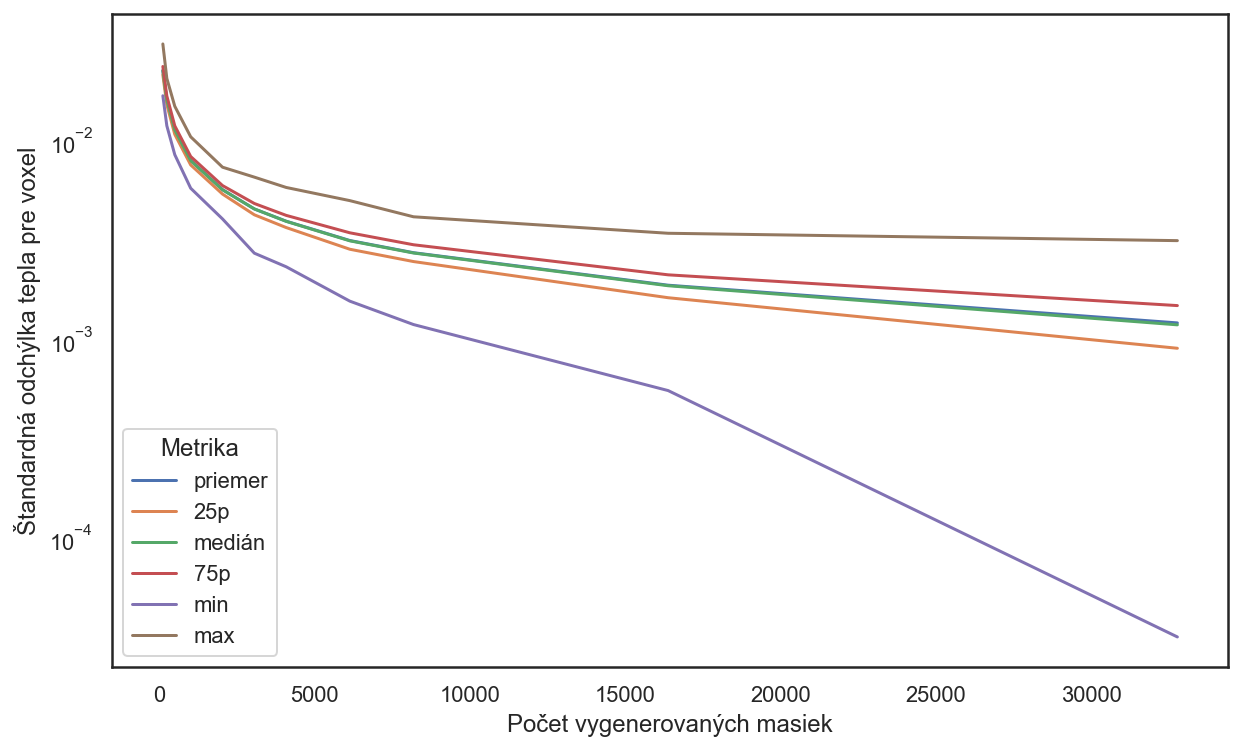
\includegraphics[width=14cm]{assets/images/risei_stability_1.png}
    \caption{Stabilita vytvorených tepelných máp podľa počtu vygenerovaných masiek. Os $y$ je v logaritmickej škále a reprezentuje chybu. Táto chyba klesá logaritmicky s vyšším počtom vygenerovaných masiek. Priemer sa veľmi blíži mediánu, preto ho na diagrame nie je takmer vôbec vidieť.}
    \label{fig:risei_stability_1}
\end{figure}

\begin{figure}[h!]
    \centering
    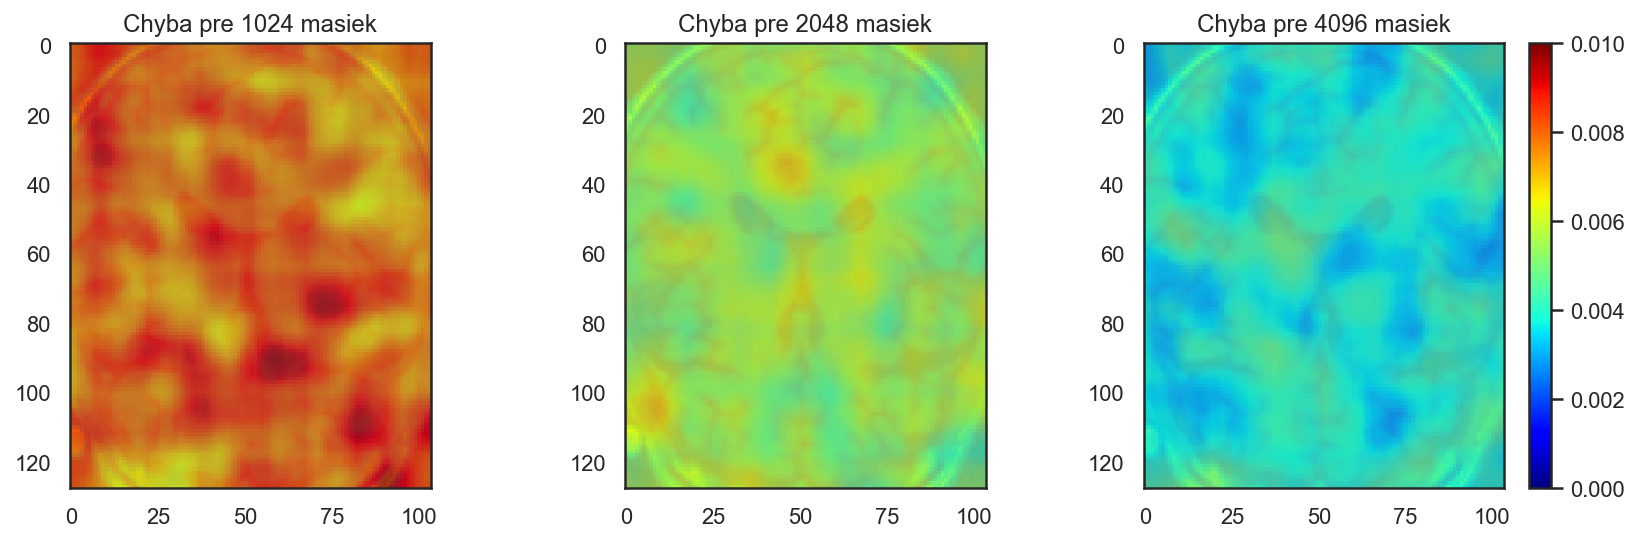
\includegraphics[width=14cm]{assets/images/risei_stability_error_visialisation.png}
    \caption{Vizualizácia chyby z generovania 1024, 2048 a 4096. Z vizualizácie je zdrejmé, že chyba je skôr náhodná ako systematická, keďže sa nachádza na rôznych častiach medzi snímkami. Škála tepla má výrazne znížené maximum oproti maximálnej možnej chybe (1) aby boli rozdiely viditeľné.}
    \label{fig:risei_stability_error_visialisation}
\end{figure}

\subsubsection{Experiment 2 (viacero snímiek)}

Keďže sme v predchádzajúcom experimente overovali stabilitu iba na jednej snímke, v tomto experimente overíme stabilitu na viacero snímkach. Z testovacej sady sme vybrali 5 TP (viď. \nameref{sec:dictionary}), 5 TN, 5 FP a 5 FN pozorovaní (tj. celkovo 20 pozorovaní), podľa toho ako ich neurónová sieť označila. Takto zabezpečíme vyváženosť tried pozorovaní v experimente. Kvôli časovej aj pamäťovej náročnosti tohto experimentu sme vytvárali 10 tepelných máp pre každé jedno pozorovanie. Výsledky boli takmer identické s predchádzajúcim experimentom (Sekcia \ref{sec:risei_stability_1}) a trend poklesu chyby pri zvyšujúcom počte masiek bol zachovaný (\ref{tab:risei_stability_2}). Z oboch experimentov vyplýva, že je vhodné použiť vyšší počet masiek pri vytváraní tepelných máp, aby sa odstránil vyplyv náhody. Ako vhodným počet považujem 2048 masiek, pri tomto počte je chyba vzhľadom na hodnoty v tejeplnej mape minimálna (Tabuľka \ref{tab:risei_stability_1}, \ref{tab:risei_stability_2}).

\begin{table}[]
    \centering
    \begin{tabular}{|r|r|}
    \hline
    \multicolumn{1}{|c|}{\begin{tabular}[c]{@{}c@{}}Počet vygenerovaných\\ masiek\end{tabular}} &
      \multicolumn{1}{c|}{\begin{tabular}[c]{@{}c@{}}Medián štandardnej\\ odchýlky pre voxel\end{tabular}} \\ \hline
    16   & 0.0594 \\ \hline
    128  & 0.0207 \\ \hline
    256  & 0.0160 \\ \hline
    512  & 0.0105 \\ \hline
    1024 & 0.0074 \\ \hline
    2048 & 0.0052 \\ \hline
    3072 & 0.0043 \\ \hline
    4096 & 0.0037 \\ \hline
    \end{tabular}
    \caption{Stabilita vytvorených tepelných máp podľa počtu vygenerovaných masiek pre 20 snímiek. Trend poklesu chyby, rovnako ako v prvom experimente, (Tabuľka \ref{tab:risei_stability_1}) ostal zachovaný.}
    \label{tab:risei_stability_2}
\end{table}

\subsection{RISE vs RISEI (s rôznymi parametrami)}

V tomto experimente sme porovnali RISE a rôzne nastavenia metódy RISEI. Použili sme model 3D CNN so senzitivitou 73\% a špecificitou 71\%.

Použili sme rovnaké nastavenie parametrov, a rovnaký počet pozorovaní ako pri výbere architektúry neurónovej siete (Sekcia \ref{sec:experiment_rise_various_architectures}) a menili sme len parametre \textit{b1}, \textit{b2} a \textit{b2\_value}. Parametre \textit{in\_paint\_radius} sme nastavili na hodnotu $5$. 

Vyhodnocovali sme len metriku \textit{insertion} (aby sme čo najrýchlejšie získali prvotné výsledky), najlepšie výsledky sme dosiahlli bez použitia dokreslenia ale s prekrytím hodnotou jedna (Tabuľka \ref{tab:experiment_risei_various_configuration}). To si vysvetľujeme tým, že hodnota voxelov blízka jednej je v trénovacej sade veľmi ojedinelá (Obr. \ref{fig:test_dataset_voxel_distribution}) a neurónová sieť na základe nich nerozhoduje, takéto voxely neurónovú sieť nepomýlia. Naopak, voxely s hodnotou/blízke hodnote nula sú pomerne časté, ak na základe nich neurónová sieť rozhoduje, može to byť dôvod prečo prekrytie zaznamenalo horšie výsledky.

Metóda s dokreslením si počínala horšie ako prekrytie hodnotou jedna, ale stále lepšie ako prekrytie s hodnotou nula pôvodná metóda RISE). Zároveň dosiahla takmer identický výsledok ako prykritie mediánom hodnôt voxelov snímky.

Obrázok \ref{fig:heatmap_and_auc_example} zobrazuje príklad vygenerovanej tepelnej mapy pre MRI snímok a výsledný graf zmeny aktivácie pre metriku \textit{insertion}. Na diagrame je vidieť, že s postupným pridávaním voxelov stúpa aktivácia pre skutočnú triedu pozorovania, takto to však nie je u všetkých pozorovaní.

\begin{figure}[h!]
    \centering
    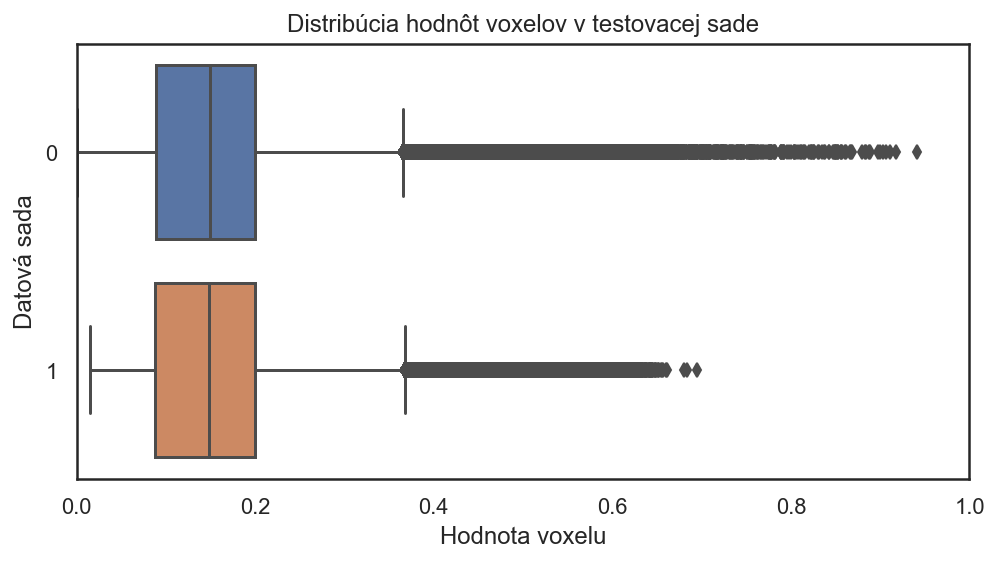
\includegraphics[width=11cm]{assets/images/test_dataset_voxel_distribution.png}
    \caption{Distribúcia hodnôt voxelov v trénovacej (0) a testovacej (1) sade. Testovacie dáta boli štandardizované (pred zmenšením) do intervalu $<0, 1>$ podľa maximálnych hodnôt v trénovacej sade.}
    \label{fig:test_dataset_voxel_distribution}
\end{figure}

\begin{table}[]
    \centering
    \begin{tabular}{l|l|l|}
        \cline{2-3}
                                                                    & \multicolumn{2}{c|}{Insertion} \\ \cline{2-3} 
                                                                    & Priemer        & Medián        \\ \hline
        \multicolumn{1}{|l|}{b1 =  0, b2 = 1, b2\_value = 0 (RISE)} & 0.43           & 0.37          \\ \hline
        \multicolumn{1}{|l|}{b1 =  0, b2 = 1, b2\_value = 1}        & \textbf{0.65}  & \textbf{0.67} \\ \hline
        \multicolumn{1}{|l|}{b1 =  0, b2 = 1, b2\_value = medián}     & 0.52           & 0.48          \\ \hline
        \multicolumn{1}{|l|}{b1 =  1, b2 = 0}                        & 0.53           & 0.47          \\ \hline
        \multicolumn{1}{|l|}{b1 =  1, b2 = 0.25, b2\_value = 0}     & 0.49           & 0.42          \\ \hline
        \multicolumn{1}{|l|}{b1 =  1, b2 = 0.50, b2\_value = 0}      & 0.44           & 0.37          \\ \hline
        \multicolumn{1}{|l|}{b1 =  1, b2 = 0.75, b2\_value = 0}     & 0.39           & 0.30          \\ \hline
    \end{tabular}
    \caption{\textbf{Porovnanie rôznych nastavení metódy RISEI.} Najlepšie výsledky dosiahla metóda bez použitia dokreslenia ale s prekrytím hodnotou jedna.}
    \label{tab:experiment_risei_various_configuration}
\end{table}

\begin{figure}[h!]
    \centering
    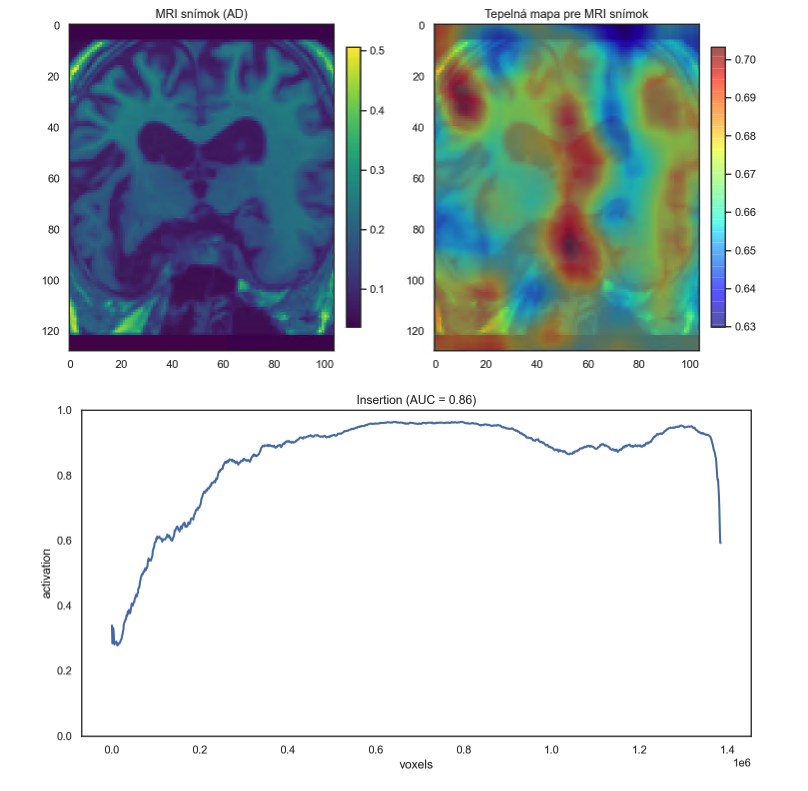
\includegraphics[width=14cm]{assets/images/heatmap_and_auc_example.png}
    \caption{Vytvorená tepelná mapa a graf zmeny aktivácie po pridávaní voxelov pre vybraný MRI snímok. Metrika AUC je pomerne vysoká, avšak je potrebné tepelnú mapu ešte vyhodnotiť z pohľadu segmentačných masiek. Tepelná mapa bola vytvorená s parametrami \textit{b1 = 1, b2 = 0} (RISEI s dokreslením).}
    \label{fig:heatmap_and_auc_example}
\end{figure}

Keďže sme neskôr natrénovali lepší model pre 3D CNN architektúru so senzitivitou 81\% a špecificitou 74\%, overlili sme ho v tomto experimente tiež, ale len na najlepšej zistenej kombinácii parametrov. Výsledok bola nižšia hodnota v metrike \textit{insertion} (priemer - 0.60, medián - 0.63). Vytvorené tepelné mapy medzi obomi modelmi boli veľmi podobné, no každý model ich vyhodnotil inak, tento problém sme načrtli v sekcii \ref{sec:experiment_rise_various_architectures}. Obrázok \ref{fig:3d_cnn_heatmap_cmp} zobrazuje takmer identicky vygenerované tepelné mapy, avšak lepší model, ktorý označil dané pozorovanie s vyššou istotou 
dosiahol nižšie skóre v metrike insertion. Tu sa črtá ďaľší problém metrík \textit{insertion} a \textit{deletion}, ak model vykazuje nižšiu mieru istoty pre pozorovanie - hodnota aktivácie, plocha pod krivkou (metrika AUC), ktorá k nej smeruje nemôže byť jedna. V našom prípade sú tieto aktivácie pomerne nízke (autori RISE uvádzali také príklady, kde aktivácie pre predikované triedy boli viac ako 0.9). Toto avšak nemusí byť nutne problém, keďže sa v snímke môžu nachádzať voxely, ktoré sú proti predikovanej triede, a teda mali nastavené teplo správne, a boli správne vložené až na konci vyhodnotenia. 

Ďaľším problémom týchto metrík môžu byť hodnoty voxelov, ktoré sú na miestach kde sme už zmazali/doposiaľ nepridali voxely, tie by mali byť neutrálne a nemali by hovoriť o žiadnej triede. My používame hodnotu nula (tá môže skôr hovoriť o AD pacientoch - chýbajúce tkanovo), avšak je tiež možné použiť opačný extrém, hodnotu jedna.

Aj kvôli zisteným problémom vyššie budeme tepelné mapy overovať voči segmentačným maskám aby sme získali lepšiu predstavu o správnosti tepelnej mapy. Aj napriek horšej metrike \textit{insertion} budeme ďalej používať lepšie natrénovaný model.

\begin{figure}[h!]
    \centering
    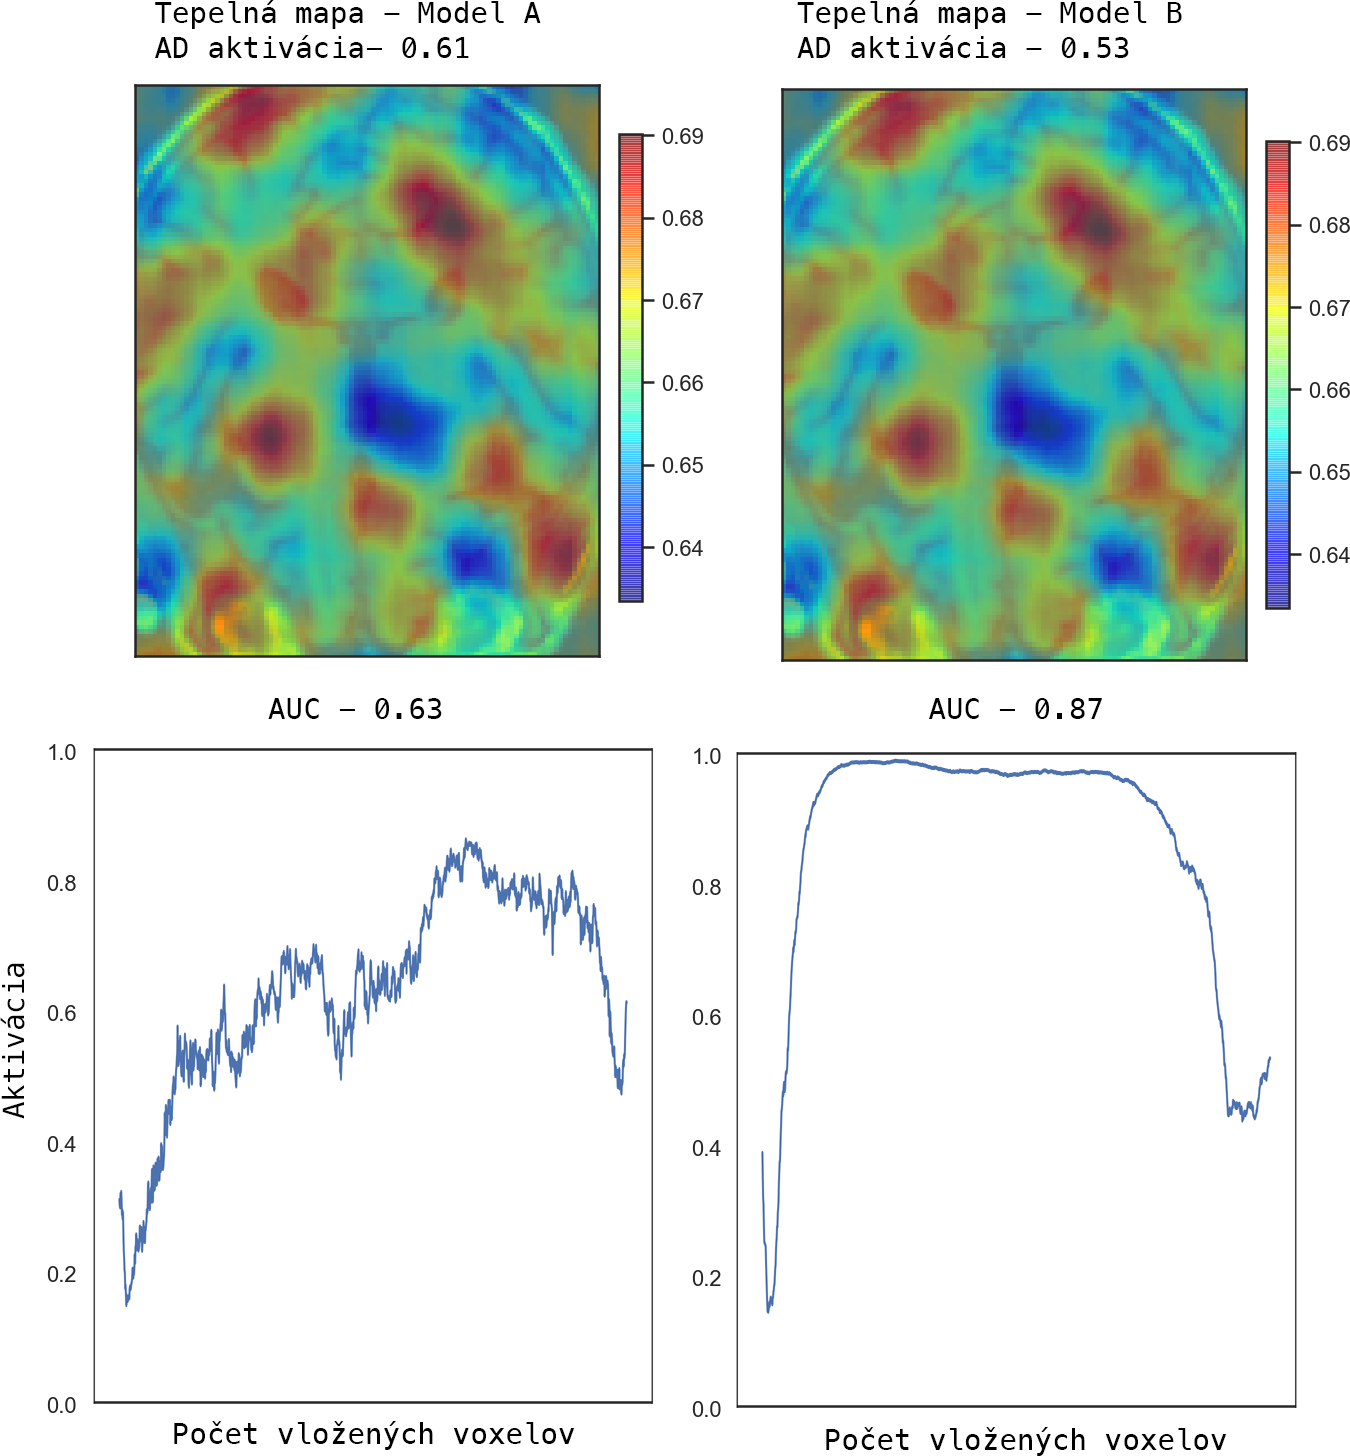
\includegraphics[width=14cm]{assets/images/3d_cnn_heatmap_cmp.png}
    \caption{Porovnanie tepelných máp vygenerovanými dvoma rôznymi modelmi. Model A) je model 3D CNN so senzitivitou 81\% a špecificitou 74\%. Model B) je model 3D CNN so senzitivitou 73\% a špecificitou 71\%. Oba modely vytvorili takmer identické tepelné mapy, avšak ich každý vyhodnotil inak. Kvalitatívne vyhodnotenie tepelnej mapy lepšie natrénovaného modelu dosiahlo horší výsledok.}
    \label{fig:3d_cnn_heatmap_cmp}
\end{figure}

\subsubsection{Nastavenie parametrov RISEI \label{sec:risei_parameters_experiment}}

Doposiaľ sme menili parametre \textit{b1}, \textit{b2} a \textit{b2\_value}, ktoré nastavujú hodnotu prekrytia v generovaných maskách. Okrem týchto parametrov má metóda RISEI ďaľšie parametre, ktoré nastavujú veľkosť prekrytia a počet generovaných masiek a významne ovplyvňujú výslednú tepelnú mapu. Vybrali sme 3 kombinácie parametrov, z predchádzajúcich experimentov, ktoré menia hodnotu prekrytia a to:

\begin{enumerate}[label=\Alph*]
    \item \textit{b1} = 0, \textit{b2} = 1 a \textit{b2\_value} = 0 (RISE),
    \item \textit{b1} = 0, \textit{b2} = 1 a \textit{b2\_value} = 1 (RISE s prekrytím hodnotou 1)
    \item \textit{b1} = 1, \textit{b2} = 0 (RISEI s dokreslením)
\end{enumerate}

čím sme zahrnuli pôvodnú metódu RISE, metódu RISEI s dokreslením a najlepšiu kombináciu parametrov. Tak ako sme uviedli v predchádzajúcom experimente, že budeme v ďaľších experiemntoch používať model 3D CNN so senzitivitou 81\% a špecificitou 74\%, tak sme sme ho aj použili. Kvoli časovej náročnsoti týchto experimentov sme použili menšiu dátovu vzorku o veľkosti 10 pozorovaní (5 AD + 5 CN).

Aj tieto experimenty potvrdili, že metóda s prekryvom hodntou jedna dosahuje najlepšie výsledky. Ďalej sme zistili, že nastavením menšieho prekryvu (parameter \textit{p} má vyššiu hodnotu) sme v kombinácii s vyšším počtom masiek dosiahli lepšie výsledky, pričom od 256 masiek boli tieto hodnoty takmer rovnaké (Obr. \ref{fig:risei_parameters}). Od 2048 masiek boli dosiahnuté výsledky takmer rovnaké, toto môže súvisieť aj so stabilitou tepelných máp pri vyšších hodnotách (Sekcia \ref{sec:risei_stability}). Metódy RISEI a RISE s prekryvom nula dosiahli najlepšie výsledky s nízkym počtom masiek. Toto je prekvapivé, vzhľadom na to, že tepelné masky z nízkym počtom masiek niesú stabilné. Je preto možné, že sa jedná o chybu a náhodu, je to preto vhodné ďaľšie skúmanie.

\begin{sidewaysfigure}
    \centering
    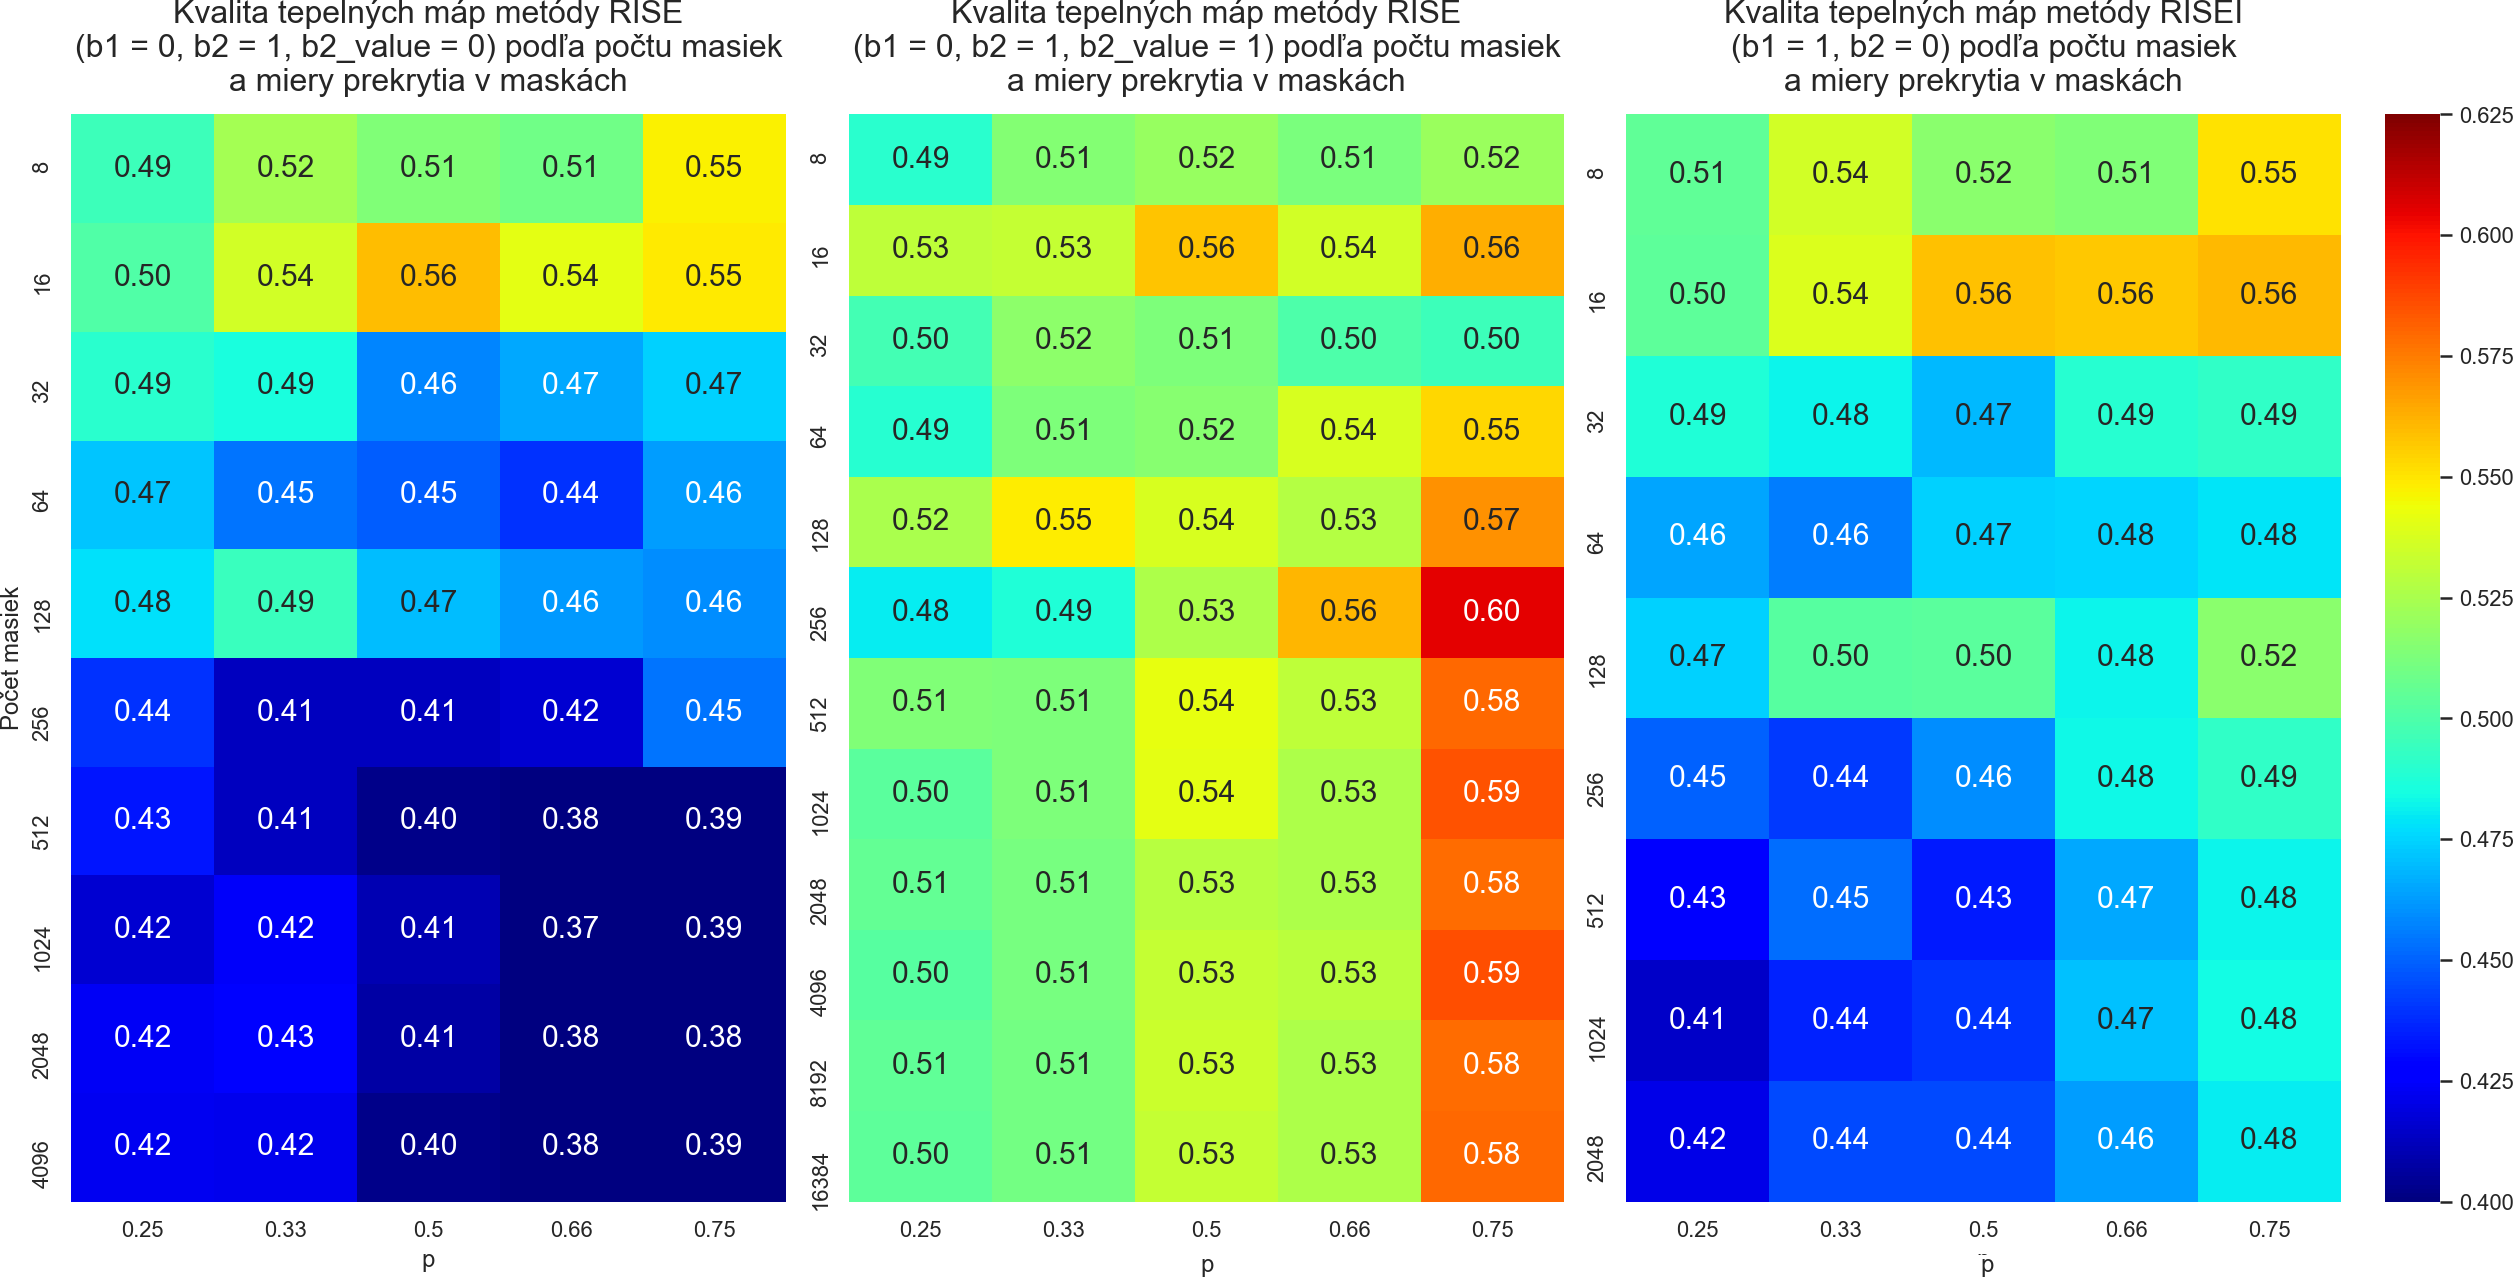
\includegraphics[width=20.6cm]{assets/images/risei_parameters.png}
    \caption{\textbf{Porovnanie kvality nastavených parametrov počtu masiek a veľkosti prekrytia (\textit{p}) na rôznych nastaveniach metódy RISEI.} Kvalitu sme merali ako $(insertion + (1 - deletion)) / 2$, z toho vyplýva, že čím vyššia hodnota, tým je vytvorená tepelná mapa kvalitnejšia. Keďže po 2048 generovaných maskách sa hodnoty výrazne nemenili (diagram v strede), tieto počty masiek sme vynechali v zvyšných experimentovh vynechali (digaramy vľavo a vpravo). Metóda RISEI s prekrytím 1 dosiahla najlepšie výsledky, zároveň vyššie hodnoty parametra \textit{p} sa ukázali ako lepšie.}
    \label{fig:risei_parameters}
\end{sidewaysfigure}

Parameter \textit{inpaint\_radius} sme za rozhodli netestovať, keďže z testov vyplynulo, že najvhodnejšie je prekrývať extrémnymi hodnotami, ktoré sú ojedinelé v dátach. Zmena tohto parametra by znamenala, že by algoritmus použil iné okolité hodnoty, tj. z nich by nevytvoril ojedinelé hodnotny.

\subsection{Porovnanie s existujúcimi metódami}

Všetky tri nastavenia metódy RISEI (vrátane metódy RISE) z predchádzajúceho experimentu (Sekcia \ref{sec:risei_parameters_experiment}) sme sa rozhodli porovnať s inými existujúcimi metódami. Na základe predchádzajúceho experimenty sme nastavili počet masiek na \textit{2048} a parameter \textit{p} na \textit{0.75}, keďže pri týchto parametroch sme dosiahli najlepšie výsledky a so zvoleným početom masiek sú tepelné mapy dostatočne stabilné (Sekcia \ref{sec:risei_stability}).

Z existujúcich metód sme vybrali metódy GradCAM, Guided Backprop a Guided GradCAM. Keďže sme sa rozhodli, že v našej práci venujeme čo najviac času experimentom a nie implementácii iných, už existujúcich metód, vybrali sme také metódy, ktoré nám ponúkala použitá knižnica \textit{captum} (preto sa neporovnávame s metódou LRP). V prípade metódy GradCAM a Guided GradCAM sme pri zväčšovaní konvolučnej vrsvy použili trilineárnu interpoláciu, keďže pracujeme s trojrozmernými dátami.

Zoznam porovnávaných metód je teda nasledovný:

\begin{enumerate}[label=\Alph*]
    \item RISE: \textit{b1} = 0, \textit{b2} = 1 a \textit{b2\_value} = 0,
    \item RISE s prekrytím hodnotou 1: \textit{b1} = 0, \textit{b2} = 1 a \textit{b2\_value} = 1,
    \item RISEI: \textit{b1} = 1, \textit{b2} = 0,
    \item GradCAM,
    \item Guided Backprop,
    \item Guided GradCAM,
    \item Guided RISE (s prekrytím hodnotou 1) - vypočítaný rovnako ako Guided GradCAM a to ako súčin tepelných máp po prvkoch medzi RISE a Guided Backprop.
\end{enumerate}

Ako testovaciu vzorku sme použili 40 pozorovaní (20 AD + 20 CN).

Vytvorené tepelné mapy sme porovnali aj oproti segmentačným maskám, v ktorých sme mali vyznačené nasledovné oblasti - šedá hmota, biela hmota, komory a hipokampus. V rámci týchto oblastí nás bude zaujímať koľko zachytili "tepla" z tepelných máp. Na základe ich veľkosti budeme následne počítať hustotu tepla ako $\frac{sucet\_tepla\_v\_oblasti}{pocet\_voxelov\_v\_ oblasti}$. Zároveň jednotlivé oblasti dáme do pomeru medzi sebou. 

\subsubsection{Metriky \label{sec:verification_experiments_metrics}}

Na vyhodnotenie tepelných máp pre každú snímku sme použili nasledovné metriky, pričom sme vychádzali z existujúcich prác popísaných v návrhu (\ref{sec:heat_maps_and_model_segmentation_masks}). 

Keďže tepelné mapy rôznych metód majú hodnoty na rôznych škálach, tepelné mapy normalizujeme a preškálujeme ich do intervalu $<0, 1>$.

\begin{enumerate}[label=\Alph*]
    \item \textit{insertion x deletion} ($(insertion + (1 - deletion)) / 2$) - vyššia hodnota je lepšia,
    \item hustota tepla v jednotlivých častiach mozgu - šedá hmota, biela hmota, komory a hipokampus - vyššia hodnota je lepšia,
    \item pomer hustoty tepla mimo mozgu oproti hustote tepla v mozgu - nižšia hodnota je lepšia,
    \item pomer hustoty tepla zvyšnej časti snímky oproti významným častiam mozgu (biela hmota, komory a hipokampus) - nižšia hodnota je lepšia,
    \item pomer hustoty tepla mimo mozgu oproti významným častiam mozgu (biela hmota, komory a hipokampus) - nižšia hodnota je lepšia.
\end{enumerate}

\subsubsection{Výsledky}

Najlepšie výsledky takmer vo všetkých metrikách (okrem metriky \textit{A} pre AD) dosiahla metóda Guided Backprop (Tabuľka \ref{tab:methods_evaluation}). 

Metriky \textit{B} je náročné porovnávať medzi metódami, keďže niektoré z nich udeľovali menej tepla (Guided Backprop), a každá z nich udeľuje teplo v iných hodnotách. Avšak dávajú nám dobrú predstavu o tom ako jednotlivé metódy rozdeľovali teplo. RISE(I) metódy rozdeľovali teplo pomerne rovnomerne (metriky B). Metóda GradCAM, a teda aj Guided GradCAM, rozdelili pomerne veľa tepla mimo mozgu (metrika C), v prípade CN pacientov to bolo až 6 násobne viac ako tepla v mozgu. U AD pacientov tomu bolo naopak a metóda Guided GradCAM dosiahla v metrike C pre AD pacientov najlepší výsledok.

V prípade Guided Backprop teplo vo významných častiach mozgu (biela hmota, komory a hipokampus) prevládalo nad teplom v ostatných častiach mozgu (metriky D a E). V prípade metód RISE(I) môžeme tvrdiť, že teplo bolo rovnomerne rozložené po celej snímke, keďže v metrikách C, D, E dosahuje hodnoty veľmi blízke $1$. 

% TODO: guided RISEI

\begin{small}
\begin{table}[]
    \begin{tabular}{|
        >{\columncolor[HTML]{C0C0C0}}l |r|r|r|r|r|r|}
        \hline
        \footnotesize{Metrika} \textbackslash \footnotesize{Metóda}                                       & \multicolumn{1}{c|}{\cellcolor[HTML]{EFEFEF}\begin{tabular}[c]{@{}c@{}}\footnotesize{Guided}\\ \footnotesize{Backprop}\end{tabular}} & \multicolumn{1}{c|}{\cellcolor[HTML]{EFEFEF}\begin{tabular}[c]{@{}c@{}}\footnotesize{Guided}\\ \footnotesize{GradCAM}\end{tabular}} & \multicolumn{1}{c|}{\cellcolor[HTML]{EFEFEF}\small{RISEI}} & \multicolumn{1}{c|}{\cellcolor[HTML]{EFEFEF}\footnotesize{GradCAM}} & \multicolumn{1}{c|}{\cellcolor[HTML]{EFEFEF}\begin{tabular}[c]{@{}c@{}}\footnotesize{RISE}\\ \scriptsize{(b2\_value}\\\scriptsize{= 1)}\end{tabular}} & \multicolumn{1}{c|}{\cellcolor[HTML]{EFEFEF}\begin{tabular}[c]{@{}c@{}}\footnotesize{RISE}\\ \scriptsize{(b2\_value}\\\scriptsize{= 0)}\end{tabular}} \\ \hline
        \small{A (AD + CN)}                                                   & \textbf{0.6779}                                                                                                 & 0.6733                                                                                                & 0.4434                                             & 0.5717                                               & 0.6101                                                                                                      & 0.4011                                                                                                      \\ \hline
        \small{A (AD)}                                                              & 0.6352                                                                                                 & \textbf{0.6690}                                                                                                & 0.4296                                             & 0.5836                                               & 0.5744                                                                                                      & 0.3844                                                                                                      \\ \hline
        \small{A (CN)}                                                              & \textbf{0.6913}                                                                                                 & 0.6734                                                                                                & 0.4529                                             & 0.5598                                               & 0.6155                                                                                                      & 0.4154                                                                                                      \\ \hline
        \begin{tabular}[c]{@{}l@{}}\footnotesize{B - nie mozog}\\ \small{(AD + CN)}\end{tabular} & 0.0186                                                                                                 & 0.0056                                                                                                & 0.5138                                             & 0.1052                                               & 0.4666                                                                                                      & 0.4864                                                     \\ \hline
        \begin{tabular}[c]{@{}l@{}}\footnotesize{B - biela hmota}\\ \small{(AD + CN)}\end{tabular} & 0.0385                                                                                                 & 0.0064                                                                                                & 0.5177                                             & 0.0597                                               & 0.4730                                                                                                      & 0.4898                                                                                                      \\ \hline
        \begin{tabular}[c]{@{}l@{}}\footnotesize{B - hipokampus}\\ \small{(AD + CN)}\end{tabular}  & 0.0306                                                                                                 & 0.0022                                                                                                & 0.5282                                             & 0.0307                                               & 0.4414                                                                                                      & 0.4806                                                                                                      \\ \hline
        \begin{tabular}[c]{@{}l@{}}\footnotesize{B - komory}\\ \small{(AD + CN)}\end{tabular}      & 0.0116                                                                                                 & 0.0013                                                                                                & 0.5061                                             & 0.0442                                               & 0.4919                                                                                                      & 0.4792                                                                                                      \\ \hline
        \begin{tabular}[c]{@{}l@{}}\footnotesize{B - šedá hmota}\\ \small{(AD + CN)}\end{tabular}  & 0.0296                                                                                                 & 0.0051                                                                                                & 0.5118                                             & 0.0610                                               & 0.4715                                                                                                      & 0.4888                                                                                                      \\ \hline
        \small{C (AD + CN)}                                                         & \textbf{0.5906}                                                                                                 & 1.1902                                                                                                & 1.0015                                             & 1.5991                                               & 0.9809                                                                                                      & 1.0049                                                                                                      \\ \hline
        \small{C (AD)}                                                              & 0.5906                                                                                                 & \textbf{0.5811}                                                                                                & 1.0026                                             & 0.8210                                               & 1.0001                                                                                                      & 0.9900                                                                                                      \\ \hline
        \small{C (CN)}                                                              & \textbf{0.5859}                                                                                                 & 4.9193                                                                                                & 0.9992                                             & 6.5940                                               & 0.9798                                                                                                      & 1.0049                                                                                                      \\ \hline
        \small{D (AD + CN)}                                                         & \textbf{0.7527}                                                                                                 & 1.1952                                                                                                & 0.9985                                             & 1.3722                                               & 0.9928                                                                                                      & 0.9996                                                                                                      \\ \hline
        \small{D (AD)}                                                              & \textbf{0.7626}                                                                                                 & 0.8400                                                                                                & 0.9940                                             & 0.9403                                               & 1.0034                                                                                                      & 0.9952                                                                                                      \\ \hline
        \small{D (CN)}                                                              & \textbf{0.7269}                                                                                                 & 3.0318                                                                                                & 1.0021                                             & 4.2573                                               & 0.9887                                                                                                      & 1.0011                                                                                                      \\ \hline
        \small{E (AD + CN)}                                                         & \textbf{0.6422}                                                                                                 & 1.2169                                                                                                & 0.9958                                             & 1.4912                                               & 0.9874                                                                                                      & 1.0028                                                                                                      \\ \hline
        \small{E (AD)}                                                             & \textbf{0.6542}                                                                                                 & 0.7034                                                                                                & 0.9946                                             & 0.8929                                               & 1.0015                                                                                                      & 0.9900                                                                                                      \\ \hline
        \small{E (CN)}                                                              & \textbf{0.6364}                                                                                                 & 3.5285                                                                                                & 0.9990                                             & 5.0326                                               & 0.9833                                                                                                      & 1.0031                                                                                                      \\ \hline
    \end{tabular}
    \caption{\textbf{Porovnanie kvality a správnosti tepelných máp RISEI oproti iným existujúcim metódam.}
    Hodnoty jednotlivých metrík sú strednými hodnotami metrik pre jednotlivé pozorovania v testovacej sade. Popis metrík sa nachadza v sekcii \ref{sec:verification_experiments_metrics}}
    \label{tab:methods_evaluation}
    \end{table}
\end{small}

\begin{figure}[h!]
    \centering
    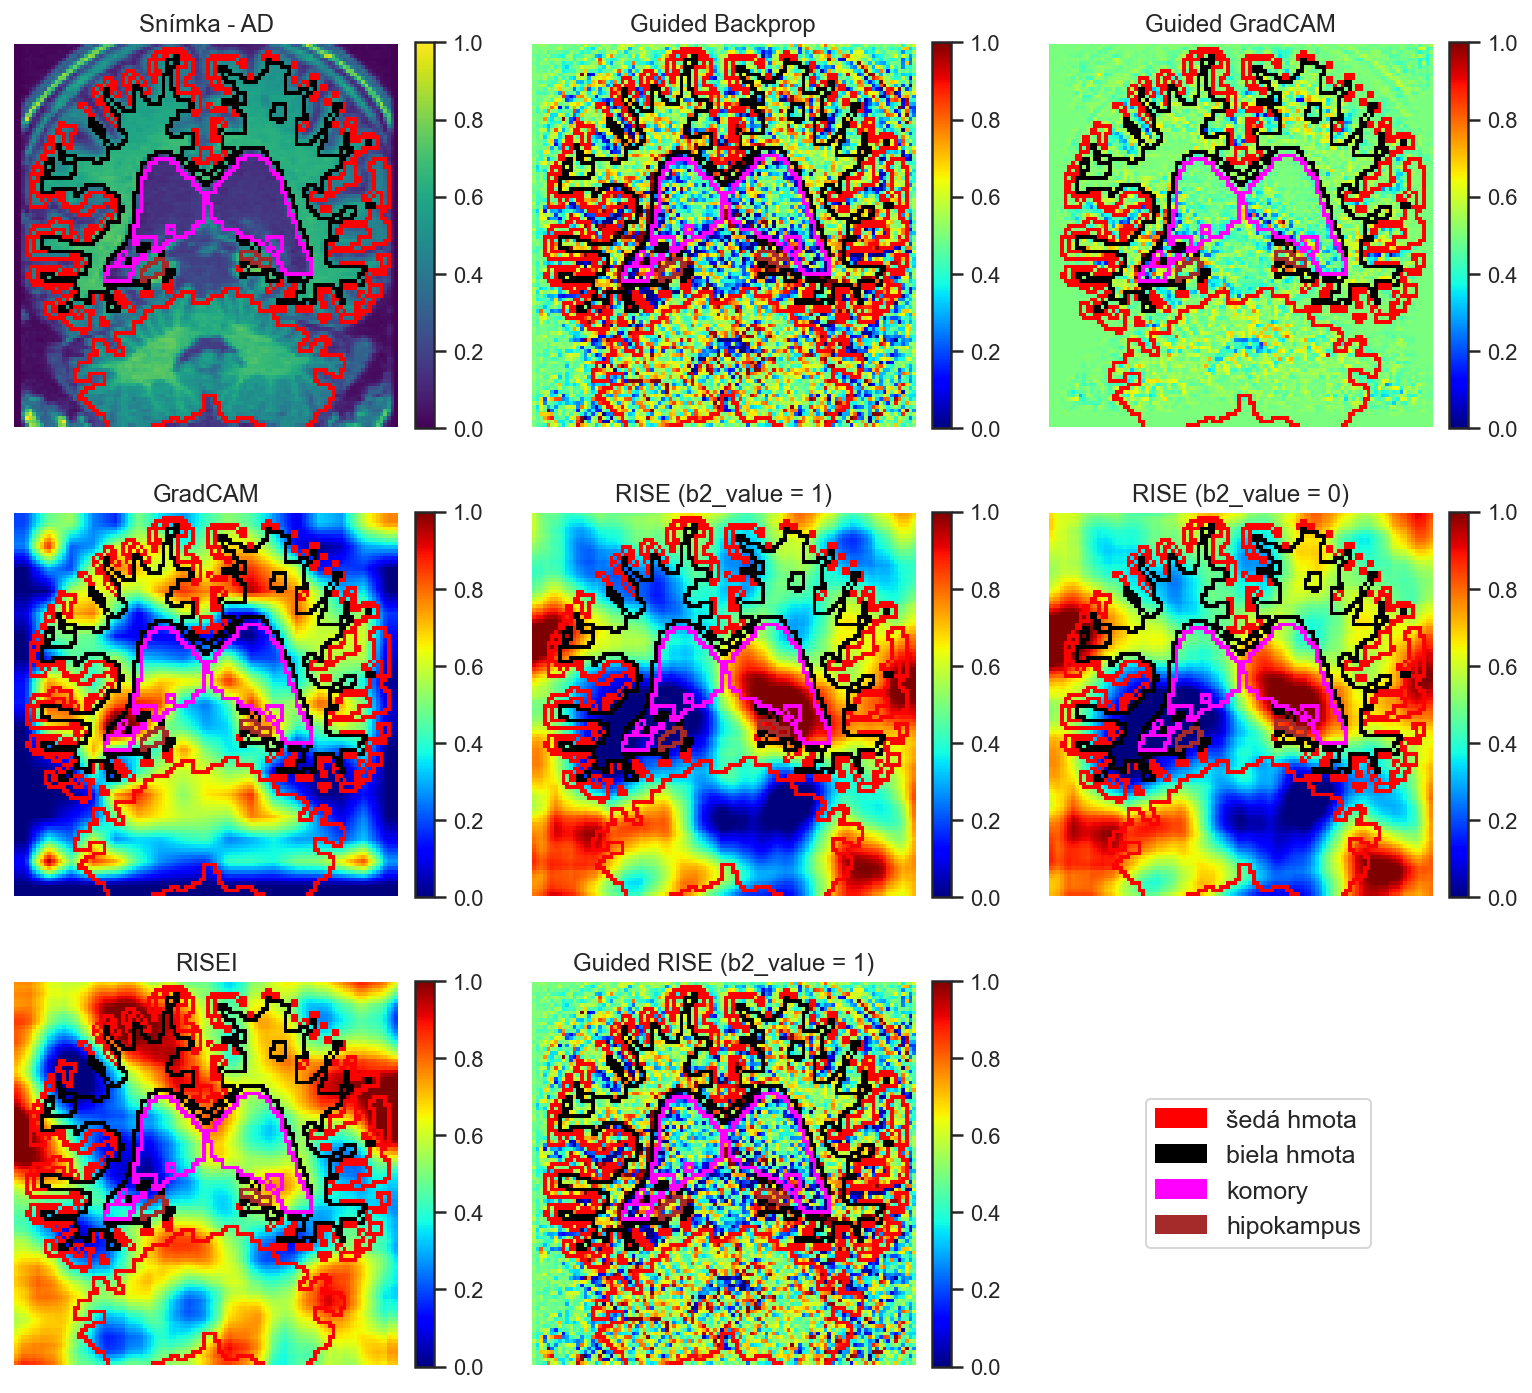
\includegraphics[width=14.5cm]{assets/images/method_evaluation_1.png}
    \caption{Porovnanie tepelných máp vygenerovaných porovnávaními metódami. Vybraný snímok má najhoršie vytvorenú tepelnú mapu pre metódu Guided Backprop podľa metriky \textit{C = 0.839}. Môžeme si všimnúť výrazné rozdiely medzi jednotlivými metódami. Všetky metódy okrem metódy Guided GradCAM uviedli značné množstvo tepla mimo oblasti mozgu. Teplo z metódy Guided Backprop, ktoré sa nachádza mimo mozgu, lemuje časť lebky, v ľavej a aj v pravej časti snímky.}
    \label{fig:method_evaluation_1}
\end{figure}

\begin{figure}[h!]
    \centering
    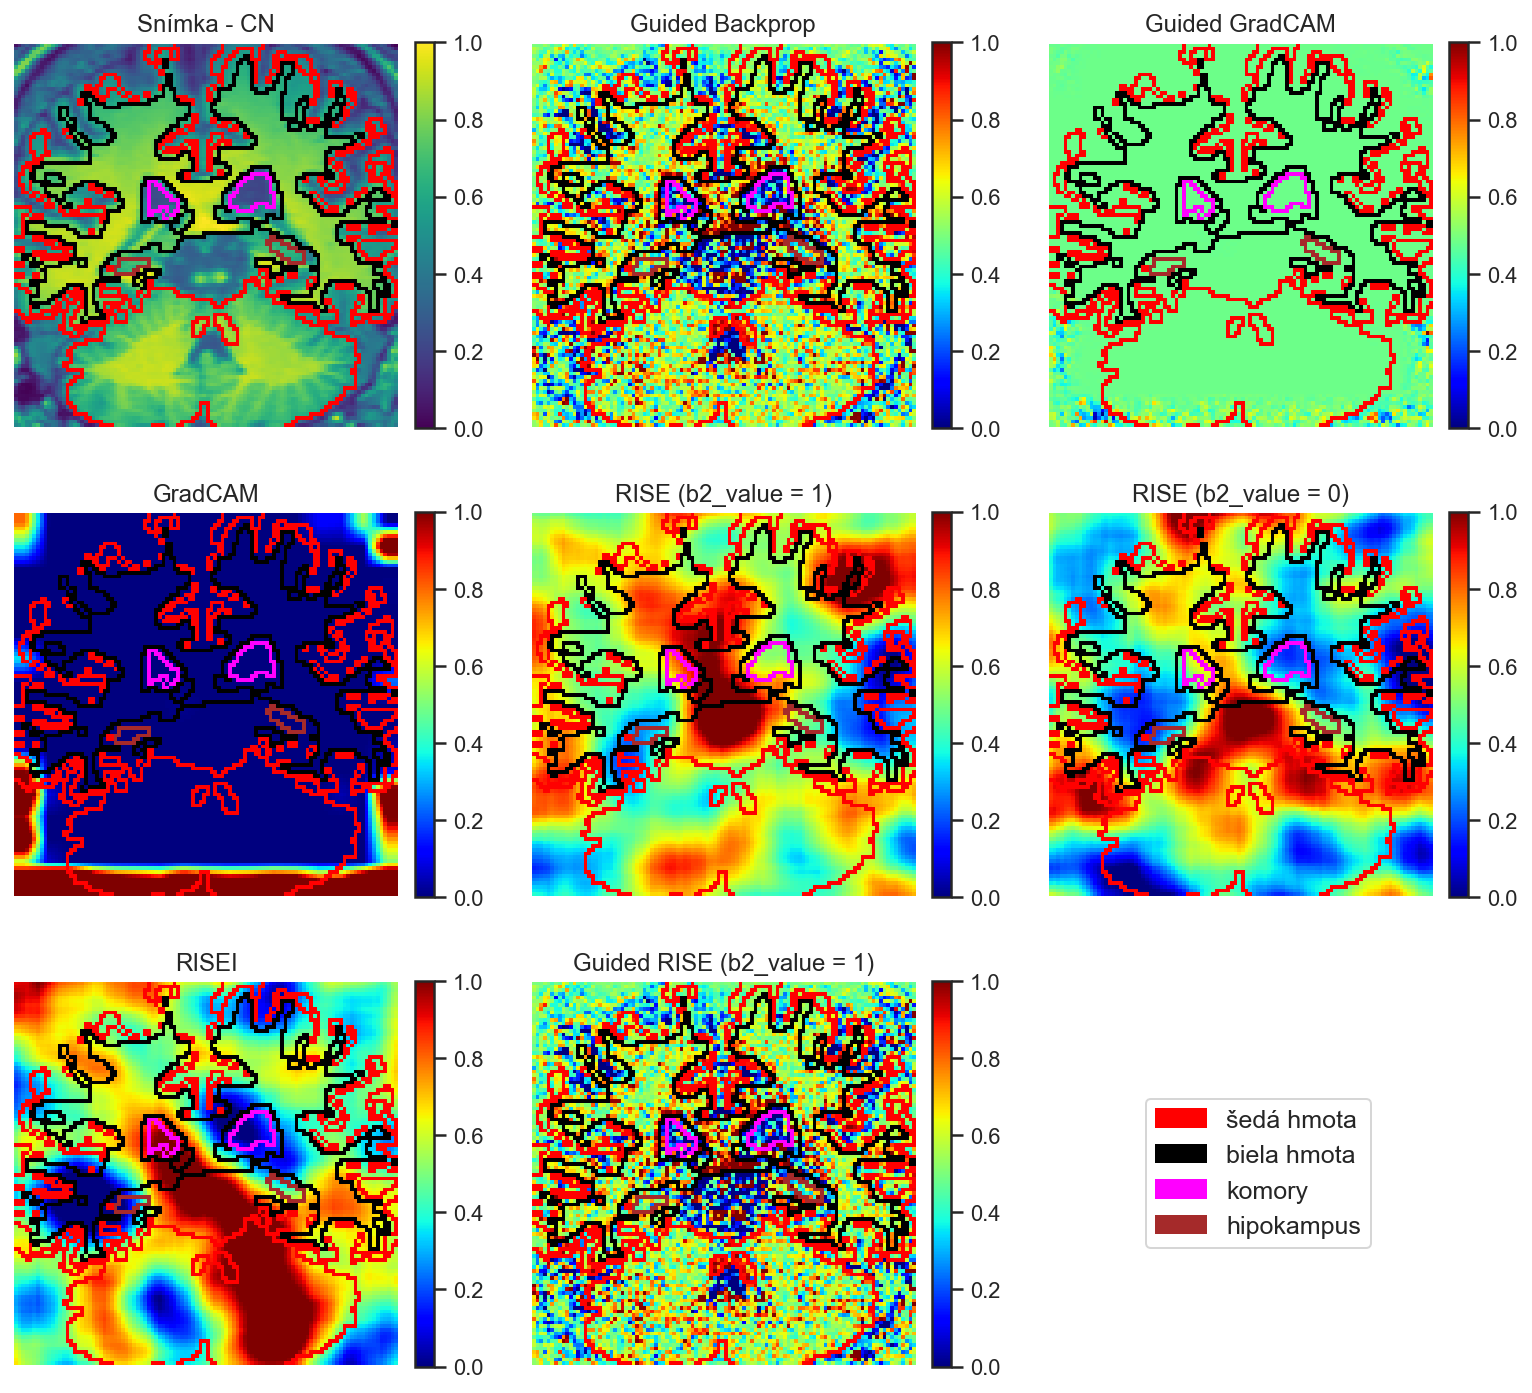
\includegraphics[width=13cm]{assets/images/method_evaluation_2.png}
    \caption{Porovnanie tepelných máp vygenerovaných porovnávaními metódami. Vybraný snímok má najlepšie vytvorenú tepelnú mapu pre metódu Guided Backprop podľa metriky \textit{C = 0.781}. Tak ako, aj na obrázku \ref{fig:method_evaluation_1}, aj tu si môžeme všimnúť výrazné rozdiely medzi jednotlivými metódami. Aj tu je viditeľné teplo lemujúce lebku v pravej časti snímky u metódy Guided Backprop. Táto časť snímky bola zachytená teplom aj metódami RISE, ale nie metódou GradCAM.}
    \label{fig:method_evaluation_2}   
\end{figure}

% TODO: compare the best and the worst heatmaps 

\section{Zhrnutie}

Metódu RISEI (a jej rôzne nastavenia) sa nám podarilo porovnať s niekoľkými existujúcimi metódami.


% Zistili sme, že metóda RISE s dokresľovaním dosahuje lepšie výsledky ako pôvodná metóda ktorá zakrývala minimálnou hodnotou. Pokial ale minimálnu hodnotu nahradíme maximálnou, dosiahneme lepšie výsledky ako s dokreslovaním, ktoré dosahuje podobné vśyeldky ako zakrývaním mediánom. Avšak, vyhodnocovali sme zatiaľ len pomerne malej vzorke a nebrali sme do úvahy početnosť tried (AD a CN) v tejto vzorke čo je nedostatkom našich experimentov (v ďaľších experimentoch by mali byť tieto triedy vyvážené). Zároveň na dátach z tejto vzorky nemali testované modely 100\%-nú úspešnosť.

% Na generovanie tepelných máp sme použili 1000 masiek (keďže autori metódy RISE v experimentoch použili podobný počet), avšak my máme iný typ dát (3D volumetrické dáta), preto je vhodné vyskúšať rôzne počty a nájsť vhodný počet pre náš problém.

% Keďže sú masky pri generovaní tepelných máp náhodné, je možné, že pre jeden MRI snímok metóda vygeneruje rôzne tepelné masky. V ďaľších experimentoch by sme mali vyhodnocovať aj konzistenciu tepelných máp - tj. ako veľmi sa líšia medzi rôznymi použitiami metódy na tom istom snímku. Predpokladáme, že väčší počet použitých másk bude viesť ku konzistentnejším tepelným mapám. Takýmto meraním môžeme dospieť k optimálnemu počtu masiek, ktorý je potrebný na generovanie tepelnej mapy.

% Taktiež je potrebné vyhodnotiť správnosť tepelných máp vzhľadom na segmentačné masky, tak ako sme uviedli v návrhu riešenia (Sekcia \ref{sec:heat_maps_and_model_segmentation_masks}). Ďalej je potrebné porovnať navrhovanú metódy s inými existujúcimi metódami, napr. LRP alebo analýza senzitivity.


% TODO: we need to compare our method with other methods like LRP or other oclussion methods
% TODO: evaluate the consistency of heatmaps, the method several times for the same image and find out if heatmaps are consistent - this way we can find also optimal number of masks
% TODO: compare with segmentation masks, if more heat is in important areas

    
    % Záver
    % \clearpage\null
    \chapter{Zhodnotenie}

V našej práci sme sa venovali uplatneniu interpretovateľnosti a vysvetliteľnosti neurónových sietí pri vyhodnocovaní medicínskych obrazových dát. 

Skúmanú doménu a problém sme si naštudovali, a zistené informácie uviedli v analýze práce. Na základe toho sme navrhli modifikáciu existujúcej metódy na vyhodnocovanie rozhodnutí neurónových sietí. Výhodou navrhnutej metódy je, že nemusí poznať použitý model, a tak je ju možné použiť aj pri komplikovanejších modeloch (napr. kombinácia neurónovej siete a inej metódy strojového učenia, model so špecifickým predspracovaním do vektoru čŕt a pod.). Zároveň sme narvhli spôsob jej overenia - vyhodnotenie a porovnanie výsledkov.

Na základe návrhu sme naimplementovali modifikáciu existujúcej metódy RISE s dokreslením pre 3D volumetrické dáta. Vytvorenú metódy sme overili v niekoľkých experimentoch na nami natrénovanom modeli. Vytvorená metóda disponuje viacerími parametrami ovplyvňujúcimi jej správanie (napr. hodnota prekrytia, miera prekrytia), preto sme v experimentoch overovali zvolené kombinácie parametrom, pričom u jednej dvojice parametrov sme prehľadávali mriežku parametrov. Keďže metóda používa na vytváranie tepelných máp masky s náhodným prekrytím, overili sme vplyv počtu vygenerovaných masiek na stabilitu tepelných máp. Metóda sa u vyššieho počtu vygenerovaných masiek ukázala ako stabilná.

Metódu sme porovnali s inými existujúcimi metódami - GradCAM, Guided Backprop a Guided GradCAM. Metóda v sledovaných metrikách dosiahla horšie výsledky ako metóda Guided Backprop, pričom dosiahla porovnateľné výsledky s metódou GradCAM. Kombináciou s Guided Backprop sme vytvorili metódu Guided RISE, ktorá dosiahla výsledky blízke Guided GradCAM a v niektorých ohľadoch takmer rovnaké s Guided Backprop. Použitie dokreslenia ako prekrytia sa neukázalo ako vhodný prístup v doméne rádiologických obrazových dát. 

Výsledné tepelné mapy sme vizualizovali. Tepelné mapy z metódy Guided Backprop naznačujú, že sa model nerozhoduje na základe relevantných častí mozgu. V ďaľších experimentoch by bolo vhodné použiť lepší model.

\subsection{Zhodnotenie cieľov práce}

\paragraph{Vytvorenie novej, alebo vylepšenie existujúcej metódy pre vysvetľovanie rozhodnutí neurónových sietí (Sekcia \ref{sec:goals_1})}

Vytvorili sme modifikáciu už existujúcej metódy RISE, do ktorej sme priniesli niekoľko funkcionálnych vylepšení - podporu pre 3D volumetrické dáta a možnosť nastavenia rôznych hodnôt prepryvu (vrátane dokreslením). Ukázalo sa, že rôzne hodnoty prekryvu majú vplyv na kvalitu tepelných máp. Navrhnutý prekryv dokreslením bol lepší oproti hodnote nula (pôvodná metóda RISE), avšak prekryv hodnotou jedna prekonal dokreslenie pričom je výpočtovo jednoduchší (Sekcia \ref{sec:verification_experiments_results}.
V doméne rádiologických dát sa dokreslenie neukázalo ako navhodnejší spôsob prekrytia.

\paragraph{Využitie vytvorenej metódy na určenie miery správnosti modelu neurónovej siete detegujúcej Alzheimerovu chorobu (Sekcia \ref{sec:goals_2})}

Vytvorenú metódu sme využili na určenie správnosti modelu tak, že vytvorené tepelné mapy sme vyhodnocovali na základe nami zadefinovaných metrík (Sekcia \ref{sec:verification_experiments_metrics}). Tieto metriky využívali segmentačné masky, ktoré overovali, či vytvorená tepelná mapa dáva zmysel z pohľadu anatómie mozgu. Výsledky ukázali, že natrénovaný model sa nerozhodoval na základe relevantných častí mozgu, čo sa odzrkadlilo v sledovaných metrikách, napr. pomer tepla mimo mozgu voči teple v mozgu.

\subsection{Limitácie}

Oproti metódam ako je GradCAM alebo Guided Backprop vytvorená metóda vyžaduje viac času na vytvorenie tepelnej mapy. Ten je variabilný a závisí od počtu masiek, veľkosti pamäte, počtu jadier a GPU. Viac výpočtových zdrojov umožňuje generovanie masiek paralelizovať a generovať vo väčších dávkach.

\subsection{Možné rozšírenia}

Ako možné rozšírenia tejto práce sme identifikovali:

\begin{itemize}
    \item Preskúmať metódu na lepšie natrénovaných modeloch (s úspešnosťami blížiacim sa k state-of-the-art), keďže vytvorená metóda bola (detailnejšie) overená iba na jednom modeli, u ktorého sme identifikovali, že sa rozhoduje na základe nie relevantných častí snímky. Takou časťou je napr. lebka, ktorý by bolo preto vhodné v predspracovaní odstrániť.
    \item Preskúmať vplyv počtu masiek na stabilitu tepelných máp, pretože to môže zredukovať ich potrebný počet a celkový čas generovania tepelných máp.
    \item Porovnať metódu s inými perturbačnými metódami, keďže sa navrhnutá metóda medzi ne zaraďuje. Navrhujeme porovnanie tepelných máp z hľadiska rýchlosti ich vytvárania a ich správnosti.
\end{itemize}

    
    % Related Work
    % \clearpage\null
    % \chapter{Related Work}

\lipsum
    
    % Resume
    % \clearpage\null
    % \chapter*{Resumé}

\lipsum
    
    % Bibliography
    \clearpage\null
    \printbibliography[
        heading=bibintoc,
        title={Literatúra},
        segment=\therefsegment,
        resetnumbers=true
    ]
    
    \end{refsegment}
    
    % Appendix
    % \appendix
    
    % \pagenumbering{gobble}
    
    \begin{appendices}
        % https://tex.stackexchange.com/questions/238781/remove-appendix-page-numbers-in-toc-while-using-appendix-package
    
        \addtocontents{toc}{
            \cftpagenumbersoff{chapter}
            \cftpagenumbersoff{section}
            \cftpagenumbersoff{subsection}
            \cftpagenumbersoff{subsubsection}
        }
    
        % \clearpage\null
        % \newpage
    
        \renewcommand{\thepage}{\arabic{page}}
    
        \chapter{Plán práce \label{cha:plan}}

\setcounter{page}{1}

\section{Letný semester - DP1}

V tomto semestri plánujem pracovať na analýze domény, návrhu metódy a jej implementácii.

\section{Zimný semester - DP2}

    % \subsection{Plán práce}
    
    V tomto semestri plánujem pracovať na implementácii navrhnutej metódy, ktorú budem overovať v experimentoch a postupne vylepšovať. V tomto semestri plánujem:
    
    \begin{itemize}
        \item natrénovať model na detekciu Alzheimerovej choroby z MRI snímkov,
        \item implementovať navrhnutú metódu,
        \item experimentovať s hyper-parametrami navrhnutej metódy,
        \item skúmať dosiahnuté výsledky, hľadať príčiny a možné vylepšenia,
        \item priebežne písať prácu -- implementáciu a dosiahnuté výsledky.
    \end{itemize}

    \subsection{Vyjadrenie k plneniu plánu}

    V tomto semestri sa nám podarilo splniť všetky stanovené ciele. Natrénovali sme niekoľko modelov detekujúcich Alzheimerovu chorobu z MRI snímkov. Čo sa týka úspešnosti týchto modelov, bohužiaľ sa nám nepodarilo dosiahnuť tak dobré výsledky ako u iných prác. Avšak, naším cieľom nie je natrénovať najlepší model, takže táto úspešnosť vyzerá byť zatiaľ pre nás postačujúca. 

    Metódu sme implementovali, tak, ako sme ju navrhli, pričom sme pridali vylepšenia ako multiprocessing - paralelné generovanie masiek.

    S hyper-parametrami navrhnutej metódy sme experimentovali (ale nie so všetkými, pretože ich je veľa), avšak sme nerobili žiadne prehľadávanie optimálnych parametrov.

    Dosiahnuté výsledky sme skúmali a diskutovali ich v závere overenia riešenia pričom sme navrhli ďalšie kroky.


\section{Letný semester - DP3}

    % \subsection{Plán práce}
    
    V tomto semestri budem pracovať na finalizácii tejto práce, navrhnutú metódu plánujem už iba vylepšovať a pracovať na záverečnom dokumente. V tomto semestri plánujem:
    
    \begin{itemize}
        \item písať prácu a jej jednotlivé časti - implementácia, technická dokumentácia, dosiahnuté výsledky, záver,
        \item vykonať úpravy v navrhnutej metóde na základe doterajších výsledkov experimentov,
        \item vyhodnotiť stabilitu tepelných máp,
        \item optimalizovať vstupné parametre do RISEI metódy,
        \item porovnať navrhnutú metódy s existujúcimi metódami,
        \item vyhodnotiť a porovnať vykonané experimenty,
        \item odovzdať prácu.
    \end{itemize}
    
    \subsection{Vyjadrenie k plneniu plánu}
    
    Plán práce sa nám v tomto semestri podarilo dodržať.
    Z experimentov nevzišli žiadne potrebné úpravy metódy, preto žiadne úpravy metódy neboli v tomto semestri vykonané. Taktiež sme vyhodnotili stabilitu tepelných máp. Rovnako sme hľadali aj optimálnu kombináciu vstupných parametrov metódy RISEI tak, že sme si vytvorili možné kombinácie parametrov, ktoré sme vyhodnotili. Neoptimalizovale sme ale všetky vstupné parametre, pri niektorých sme uznali, že to u nich nedáva zmysel. Vytvorenú metódu sme taktiež porovnali s existujúcimi metódami GradCAM, Guided Backprop a Guided GradCAM. Vykonali sme veľké množstvo experimentov (rôzne parametre RISEI, kombinácia RISEI a guided backprop atď.), ktoré sme vyhodnotili (napr. vyhodnotenie na segmentačných maskách) a porovnali.

    
        \clearpage\null
        \chapter{Technická dokumentácia \label{cha:technical_documentation}}

\setcounter{page}{1}

Metóda RISEI je implementovaná v jazyku Python, rovnako ako aj jej vyhodnotenie
a porovnanie s ostatnými metódami.

\section{Príprava vývojového prostredia}

Na správu python-ovských balíkov a vývojového prostredia je použitá \href{https://docs.conda.io/projects/conda/en/latest/index.html}{conda}, ktorú je nutné nainštalovať. Condu je možné nainštalovať cez distribúciu \href{https://www.anaconda.com/anaconda/}{Anaconda} (Anaconda obsahuje grafické rozhranie a množstvo nástrojov/programov) alebo menšiu distribúciu \href{https://docs.conda.io/en/latest/miniconda.html}{Miniconda}. V prípade, že potrebujete šetriť miesto na disku, odporúčam menšiu distribúciu Miniconda.

Po inštalácii condy zadajte nasledovný príkaz v koreňovom adresári repozitára. Tento príkaz vytvorí nové conda prostredie v ktorom nainštaluje potrebné python balíky.

\begin{lstlisting}[style=BashInputStyle]
    $ conda env create -f environment.yml
\end{lstlisting}

Následne pre aktiváciu conda prostredia zadajte nasledovný príkaz.

\begin{lstlisting}[style=BashInputStyle]
    $ conda activate dp-timzatko
\end{lstlisting}

Teraz je možné používať shell, v ktorom bolo aktivované conda prostredie \textit{dp-timzatko}, na spúšťanie Python skriptov a Jupyter notebookov.

Následne spustite Jupyter notebook klienta.

\begin{lstlisting}[style=BashInputStyle]
    $ jupyter-notebook
\end{lstlisting}

Teraz je možné, prezerať, spúšťať a upravovať jupyter notebooky v repozitári.

\section{Závislosti (použité knižnice)}

Na implementáciu riešenia sme použili nasledovné Python knižnice (uvádzame len tie najvýznamnejšie). Kompletný zoznam sa nachádza v súbore \textit{[REPOZITÁR]/environment.yml}.

\begin{itemize}
    \item numpy - na prácu s vektormi, maticami a matematickými operáciami nad nimi.
    \item pandas - na vytváranie, a ukladanie tabuľkami.
    \item seaborn - vykresľovanie grafov.
    \item matplotlib - vykresľovanie rádiologických snímkov, tepelných mám a segmentačných masiek.
    \item opencv - na dokreslenie v RISEI.
    \item tensorflow (v2.3.1), tensorboad - implementácia, trénovanie, evaluácia modelu na predikciu alzheimerovej choroby.
    \item torch, torchvision - evaluácia modelu na predikciu alzheimerovej choroby. Pytorch je potrebný, pretože je závislosťou knižnice \textit{captum}, ktorú používame na vytváranie tepelných masiek existujúcimi metódami (GradCAM a pod.).
    \item SimpleITK - načítanie volumetrických dát z disku.
    \item scikit-image - práca s vizuálnymi dátami (augmentácie, zmena veľkosti).
\end{itemize}

\section{Technické riešenie}

Implementácia riešenia (RISEI, model, evaluácia atď.) sa nachádza v adresári \textit{[REPOZITÁR]/src}. Funkcionalita z tohto adresára je následne importovaná jupyter notebookmi v adresári \textit{[REPOZITÁR]/conda\_notebooks}. Každý z notebookov má iný účel - trénovanie modelu, vyhodnotenie metódy RISEI, porovnanie metód a pod (detailný opis k týmto notebookom sa nachádza v prílohe \ref{cha:cdrom} Opis digitálnej časti práce).

\section{Moduly}

Adresár \textit{[REPOZITÁR]/src} obashuje nasledovné Python moduly, ktoré majú uvedené zodpovednosti.

\begin{itemize}
    \item \textbf{src.risei} - implementácia metódy RISEI (exportuje triedu RISEI) - generovanie masiek.
    \item \textbf{src.model} - obsahuje pomocné funkcie na prácu s tensorflow modelom (načítanie checkpointu atď.). 
    \item \textbf{src.model.cnn\_3D} - implementácia 3D konvolučnej neurónovej siete v tensorflow-e.
    \item \textbf{src.model.res\_net} - implementácia 3D a 2D siete ResNet v tensorflow-e.
    \item \textbf{src.model.compile\_model} - kompilácia tensorflow modelu a nastavenie metrík, optimizéru, chybovej funkcie a predvolených nastavení.
    \item \textbf{src.model.create\_model} - vytvorenie modelu.
    \item \textbf{src.model.training} - spustenie trénovania modelu, vrátane vytvorenie tensorflow datasetu, nastavenia augmentácií, pripojenia k tensorboardu a pod. na základe vstupných parametrov.
    \item \textbf{src.model.mri\_tensorboad\_callback} - výpis rádiologických snímkov po epochách/iteráciách do tensorboard-u pri trénovaní.
    \item \textbf{src.model.evaluation} - vyhodnotenie modelu (matica zmätenia, klasifikačné metriky) a priebehu jeho trénovania.
    \item \textbf{src.model.torch.cnn\_3D} - implementácia 3D konvolučnej neurónovej siete v pytorch-y.
    \item \textbf{src.data} - práca s volumetrickými dátami, konverzia tensorflow sequence do numpy a opačne.
    \item \textbf{src.data.description} - popisné štatistiky o dátovej sade.
    \item \textbf{src.data.augmentations} - augmentácie.
    \item \textbf{src.data.mri\_sequence} - načítanie MRI snímkov, štítkov a segementačných masiek z disku. Zmena veľkosti snímkov, orezanie snímkov, štandardizácia dát, rozdelenie dát do dávok.
    \item \textbf{src.data.train\_test\_split} - rozdelenie dátovej sady na trénovaciua, testovaciu a validačnú.
    \item \textbf{src.data.selector} - výber záznamov z dátovej sadny na základe triedy AD/CN a správnosti klasifikácie modelom.
    \item \textbf{src.data.evaluation.segmentation\_masks} - evaluácia tepelných máp podľa segmentačných masiek.
    \item \textbf{src.heatmaps} - generovanie tepelných máp.
    \item \textbf{src.heatmaps.evaluation} - evaluácia kvality tepelnej mapy podľa metrík \textit{insertion} a \textit{deletion}, perzistencia histórie - tepelných máp a ich evaluácie, načítanie histórie evaluácie, vizualizácie v diagramoch. 
\end{itemize}

Funkcie a triedy v moduloch sú v primeranom rozashu dokumentované pomocou komentárov. Ďalej bližšie opíšeme najviac dôležitý modul implementujúci navrhnutnú metódu \textit{RISEI}.

\subsection{Modul: src.risei}

Tento modul poskytuje triedu RISEI ktorá slúži na generovanie masiek, z ktorých sa vytvárajú tepelné mapy.

\subsubsection{Trieda: RISEI}

Trieda RISEI slúži na generovanie masiek.

\begin{lstlisting}
    class src.risei.RISEI(input_size, s=8, p1=0.5, b1=0.8, b2=0.5,
        b2_value=0,
        in_paint='2d',
        in_paint_radius=20,
        in_paint_algorithm=cv2.INPAINT_NS,
        in_paint_blending=True,
        in_paint_2d_to_3d=False,
        processes=4,
        debug=False,
    )
\end{lstlisting}

\paragraph{Parametre}

\begin{itemize}
    \item \textbf{s} - veľkosť mriežky, z ktorej sa vytvára binárna maska.
    \item \textbf{p1} - pravdepodobnosť, že pixel v mriežke bude biely.
    \item \textbf{b1} - miera prekryvu medzi pôvodným obrázkom a dokreslením. Ak je \textit{0} tak sa dokreslenie vôbec nevykoná.
    \item \textbf{b2} - miera prekryvu medzi pôvodným obrázkom s dokreslením a ''čiernou'' maskou. 
    \item \textbf{b2\_value} - hodnoty v ''čiernej'' maske.
    \item \textbf{in\_paint} - typ dokreslenia. Môže byť \textit{2d} alebo \textit{3d}. V prípade \textit{2d} je dokreslenie realizované iba v prvej dimenzii.
    \item \textbf{in\_paint\_radius} - rádius dokreslenia (posúva sa ďalej do knižnice \textit{opencv}).
    \item \textbf{in\_paint\_algorithm} - algoritmus dokreslenia, môže byť \textit{cv2.INPAINT\_NS} alebo \textit{cv2.INPAINT\_TELEA}.
    \item \textbf{in\_paint\_blending} - ak \textit{True} dokreslenie bude prekryté s pôvodným snímkom podľa interpolovanej čiernej masky (tak nevzniknú žiadne ostré hrany).
    \item \textbf{processes} - počet procesov v ktorých sa budú generovať masky.
    \item \textbf{debug} - ak \textit{True} budú do pamäte ukladané medzivýsledky z generovania masiek (binárna maska, interpolovaná maska atď.).
\end{itemize}

\paragraph{Metódy}

Metódy triedy RISEI.

\vspace{8pt}
\begin{lstlisting}
    generate_masks(n, image, log=True, seed=None)
\end{lstlisting}

Metóda vygeneruje masky k poskytnutej snímke ($image$).

Parametre:
\begin{itemize}
    \item \textbf{n} - počet masiek na vygenerovanie,
    \item \textbf{image} - 3D snímka \textit{(x, y, z)} (k nej budú vygenerované masky),
    \item \textbf{log} - ak \textit{True} na štandardnom výstupe bude zobrazený aktuálny stav generovania masiek,
    \item \textbf{seed} - seed pre náhodu.
\end{itemize}

\vspace{32pt}
\begin{lstlisting}
    show_from_last_run(i, z, figsize=(12, 8), dim=0):
\end{lstlisting}

Parametre:
\begin{itemize}
    \item \textbf{i} - i-ta maska na zobrazenie,
    \item \textbf{z},
    \item \textbf{figsize} - veľkosť vykresleného diagarmu,
    \item \textbf{dim} - reprezentuje rozmer - 0, 1, 2.
\end{itemize}

\subsection{Modul: src.heatmaps.evaluation}

Temto modul poskytuje generovanie a evaluáciu kvality tepelnej mapy podľa metrík \textit{insertion} a \textit{deletion}, perzistenciu histórie - tepelných máp a ich evaluácie, načítanie histórie a vizualizácie v diagramoch.

\subsubsection{Trieda: HeatmapEvaluationV3}

Táto trieda vytvorí a vyhodnotí tepelné mapy, následne vráti históriu evaluácie.

\begin{lstlisting}
    class src.risei.HeatmapEvaluationV3(
        predict_fn,
        heatmap_fn,
        sequence,
        evaluation_step_size=1000,
        evaluation_max_steps=-1,
        evaluation_batch_size=32)
\end{lstlisting}

\paragraph{Parametre}

\begin{itemize}
    \item \textbf{predict\_fn} - funkcia \textit{def predict\_fn(batch\_x)}, ktorá pre dávku snímkov vráti pravdepodobnosti predikovaných pre jednotlivé triedy.
    \item \textbf{heatmap\_fn} - funkcia \textit{heatmap\_fn(image\_x, image\_y, evaluation\_idx, seed, log}, ktorá vráti tepelnú mapu pre snímku \textit{image\_x}.
    \item \textbf{sequence} - sekvencia snímok - musí byť \textit{src.data.MRISequence}.
    \item \textbf{evaluation\_step\_size} - koľko voxelov bude vložených v jednom kroku pri evaluácii tepelnej mapy. 
    \item \textbf{evaluation\_batch\_size} - koľko snímkov vkladať pri evaluácii do modelu.
\end{itemize}

\paragraph{Metódy}

Metódy triedy HeatmapEvaluationV3.

\vspace{8pt}
\begin{lstlisting}
    evaluate(log=False, verbose=0, seed=None)
\end{lstlisting}

Spustí generovanie a evaluáciu tepelných máp. Metóda vráti \textit{src.heatmaps.\-evaluation.\-Heatmap\-EvaluationHistory} s históriou evaluácie a s metrikami.

Parametre:
\begin{itemize}
    \item \textbf{log} - zapne alebo vypne výpisy.
    \item \textbf{verbose} - úroveň výpisov 0, 1, 2 (najmenej až najviac).
    \item \textbf{seed} - seed pre náhodu (posunutý do \textit{heatmap\_fn}).
\end{itemize}

\subsubsection{Trieda: HeatmapEvaluationHistory}

Táto uchováva históriu evaulácie tepelných máp. Umožňuje ich načítavať a ukladať na disk.

\begin{lstlisting}
    class src.risei.HeatmapEvaluationHistory(
        method, auc, arr_auc, arr_heatmap, arr_x, arr_y, arr_y_pred, arr_y_pred_heatmap,
                 arr_voxels, arr_max_voxels, arr_step_size)
\end{lstlisting}

Túto triedu inicializuje knižnica (v \textit{src.heatmaps.\-evaluation.\-HeatmapEvaluationV3}), nemal by ju inicializovať klientský kód.

\paragraph{Metódy}

Metódy triedy HeatmapEvaluationHistory.

\vspace{8pt}
\begin{lstlisting}
    save(path, filename)
\end{lstlisting}

Uloží históriu na disk.

Parametre:
\begin{itemize}
    \item \textbf{path} - cesta k súboru.
    \item \textbf{filename} - názov súboru.
\end{itemize}

\vspace{24pt}
\begin{lstlisting}
    @staticmethod
    def load(path, filename):
\end{lstlisting}

Načíta históriu z disku.

Parametre:
\begin{itemize}
    \item \textbf{path} - cesta k súboru.
    \item \textbf{filename} - názov súboru.
\end{itemize}

\vspace{24pt}
\begin{lstlisting}
    description(percentage=True, cls_index=None)
\end{lstlisting}

Vypíše popisné štatistiky (min, max, priemer, štandardná odchýlka) pre plochy pod krivkou jednotlivých evaluácií.

Parametre:
\begin{itemize}
    \item \textbf{percentage} - ak $False$ vráti AUC v absolútnych číslach vzhľadom na počet voxelov a nie hodnotu z intervalu $<0, 1>$.
    \item \textbf{cls\_index} - ak $None$ vráti štatistiky pre všetky pozorovanie, ak číslo, vráti štatistiky pre index danej triedy.
\end{itemize}

Táto trieda poskytuje aj ďaľšie metódy pre vizualizáciu plochy pod krivkou pre jednotlivé pozorovania a pod., popísali sme iba najdôležitejšie z nich.

\paragraph{Atribúty}

\begin{itemize}
    \item \textbf{arr\_heatmap} - vygenerované tepelné mapy pre všetky snímky.
    \item \textbf{arr\_x} - snímky.
    \item \textbf{arr\_y} - skutočne triedy ku snímkam.
    \item \textbf{arr\_y\_pred} - predikované triedy ku snímkam.
    \item \textbf{arr\_auc} - hodnoty AUC pre jednotlivé snímky.
\end{itemize}

\thispagestyle{empty}
\mbox{}
\newpage
    
        \clearpage\null
        \chapter{Opis digitálnej časti práce \label{cha:cdrom}}

\setcounter{page}{1}

Evidenčné čislo práce v informačnom systéme FIIT-182905-86077.

Obsah digitálnej časti práce (archív ZIP):

\begin{itemize}
    \item \texttt{/DP\_TimotejZatko.pdf} --- Práca vo formáte PDF.
    \item \texttt{/DP\_prilohy\_TimotejZatko.pdf} --- Prílohy vo formáte PDF.
    \item \texttt{/repo.zip} --- Zdrojové súbory a dáta vo formáte ZIP.
\end{itemize}

Obsah súboru \texttt{repo.zip}:

\begin{itemize}
    \item \texttt{/repo/thesis/} --- Zdrojové súbory práce vo formáte \LaTeX.
    \item \texttt{/repo/tmp/} --- Dátová sada, zoserializované natrénované modely, záznamy z trénovania modelov, zoserializované výsledky experimentov. 
    \item \texttt{/repo/src/} --- Všetky zdrojové súbory, vrátane metódy RISEI, modelov, generovania tepelných máp. Obsahuje Python balíky.
    \item \texttt{/repo/scripts/} --- Pomocný skript na stiahnutie dát z Google Drive.
    \item \texttt{/repo/assets/} --- Zdrojové súbory diagramov použitých v práci. 
    \item \texttt{/repo/colab\_notebooks/} --- Obsahuje Jupyter notebooky z trénovania modelov na platforme Google Colab s vyuŽitím GPU aj TPU (obsahuje prvé natrénované modely) 
    \item \texttt{/repo/conda\_notebooks/} --- Obsahuje Jupyter notebooky.
    \item \texttt{/repo/conda\_notebooks/dataset.ipynb} --- Rozdelenie dátovej sady.
    \item \texttt{/repo/conda\_notebooks/tensorboad.ipynb} --- Tensorboad.
    \item \texttt{/repo/conda\_notebooks/augmentations.ipynb} --- Vizualizácia implementovaných augmentácií.
    \item \texttt{/repo/conda\_notebooks/training/training\_history.ipynb} --- Vizualizácia priebehu trénovania.
    \item \texttt{/repo/conda\_notebooks/training/augmentations/} --- Porovnanie vplyvu augmentácií na výsledný model. 
    \item \texttt{/repo/conda\_notebooks/training/2d\_ResNet18/} --- Trénovanie modelu 2D ResNet18 (viacero jupyter notebookov).
    \item \texttt{/repo/conda\_notebooks/training/3d\_ResNet18/} --- Trénovanie modelu 2D ResNet18 (viacero jupyter notebookov).
    \item \texttt{/repo/conda\_notebooks/training/3d\_cnn/} --- Trénovanie modelu 3D CNN (viacero jupyter notebookov).
    \item \texttt{/repo/conda\_notebooks/risei/model\_comparison\_v1/} --- Porovnanie metódy RISEI a jej parametrov na natrénovaných modeloch (prvá iterácia, staré modely, viacero jupyter notebooko).
    \item \texttt{/repo/conda\_notebooks/risei/model\_comparison\_v2/} --- Porovnanie metódy RISEI a jej parametrov na natrénovaných modeloch (druhá iterácia, nové modely, viacero jupyter notebookv).
    \item \texttt{/repo/conda\_notebooks/risei/evaluation\_history\_ins\_del\-.ipynb} --- Vypísanie štatistík pre vybranú evaluáciu metódy.
    \item \texttt{/repo/conda\_notebooks/risei/evaluation\_history\_ins\_del\-\_comparison\-.ipynb} --- Porovnanie vybraných dvoch evaluácii metód.
    \item \texttt{/repo/conda\_notebooks/risei/evaluation\_history\_\-segmentation\-\_masks\-.ipynb} --- Vyhodnotenie metódy voči segmentačným maskám.
    \item \texttt{/repo/conda\_notebooks/risei.evalution\_all.ipynb} --- Porovnanie všetkých experimentov.
    \item \texttt{/repo/conda\_notebooks/risei/risei.ipynb} --- RISEI - zobrazenie generovaných masiek podľa nastavených parametrov.
    \item \texttt{/repo/conda\_notebooks/risei/experiments/methods/} --- Vyhodnotenie tepelných máp z iných, existujúcich metód (viacero jupyter notebookov).
    \item \texttt{/repo/conda\_notebooks/risei/experiments/parameters/} --- Hľadanie optimálneho počtu parametrov (viacero jupyter notebookov).
    \item \texttt{/repo/conda\_notebooks/risei/experiments/stability/} --- Vyhodnotenie kvality stability tepelných máp podľa počtu vygenerovaných masiek (viacero jupyter notebookov).
\end{itemize}

Digitálna časť práce má veľkosť 123.9 GB, kvôli čomu je uložená v systéme G Suite for
Education.
Názov odovzdaného archívu: \texttt{DP3\_TimotejZatko.zip}

    
        % \clearpage\null
        % \chapter{Výskumný článok a poster na IIT.SRC 2019 \label{cha:research_article}}

\setcounter{page}{1}

Výskumný článok a poster, ktorý vznikol na základe tejto práce na konferenciu IIT.SRC 2019.

\includepdf[pages={1,2,3,4}]{../iit.src-article/main.pdf}

\includepdf[pages={1}]{../iit.src-poster/bp.pdf}

\thispagestyle{empty}
\mbox{}
\newpage
    \end{appendices}
\end{document}
